% =========================================================================================
% POCUS-Emergency -- End-of-Studies Internship Report
% Compile with: pdflatex -> biber -> pdflatex -> pdflatex   (or latexmk -pdf main.tex)
% =========================================================================================
\documentclass[11pt, a4paper]{article}

% =========================================================================================
% preamble.tex -- packages, page style and shared commands
%
% Kept deliberately light. Overleaf's free plan caps total compile time, and a full build
% runs pdflatex -> biber -> pdflatex -> pdflatex, so every package is paid for three times.
% Two packages were removed for this reason:
%   glossaries -- \printnoidxglossary sorts with TeX macros and is very slow; replaced by
%                 the lightweight acronym mechanism in glossary.tex
%   microtype  -- improves justification, costs time on every pass
% Both can be restored if the project ever moves to a local TeX installation.
% =========================================================================================

\usepackage[utf8]{inputenc}
\usepackage[T1]{fontenc}
\usepackage[english]{babel}
\usepackage{lmodern}
\usepackage[a4paper, margin=2.5cm]{geometry}

\usepackage{amsmath, amssymb}
\usepackage{graphicx}
\usepackage{float}
\usepackage{booktabs}
\usepackage{tabularx}
\usepackage{enumitem}
\usepackage{xcolor}

% caption must be loaded ONCE. Loading it twice with different options
% (\usepackage[figurename=Fig.]{caption} then \usepackage[tablename=Tab.]{caption})
% raises an option clash error.
\usepackage[figurename=Fig., tablename=Tab., font=small, labelfont=bf]{caption}

\usepackage{fancyhdr, lastpage}
\usepackage[hidelinks]{hyperref}
\usepackage[backend=biber, style=numeric, sorting=none]{biblatex}
\usepackage{csquotes}   % biblatex warns without it when babel is loaded

\graphicspath{{figures/}{logos/}}

% ---------------------------------------------------------------------------- colours ---
\definecolor{accent}{HTML}{1F4E79}
\definecolor{softgrey}{HTML}{595959}

% ----------------------------------------------------------------------- page styles ---
\fancypagestyle{plain}{%
  \fancyhf{}
  \fancyhead[L]{\small\itshape Mariem Brik}
  \fancyhead[R]{\small\itshape POCUS-Emergency}
  \fancyfoot[L]{\small\itshape University year 2025--2026}
  \fancyfoot[R]{\small\thepage\ / \pageref{LastPage}}
  \renewcommand{\headrulewidth}{0.4pt}
  \renewcommand{\footrulewidth}{0.4pt}
}
\pagestyle{plain}

% ------------------------------------------------------------------ shared commands ---
% A statement set apart from the body text: used for the research question and for the
% principles the architecture rests on.
\newenvironment{keystatement}{%
  \par\medskip\noindent
  \begin{minipage}{\linewidth}
    \color{accent}\itshape\bfseries
    \leftskip=1.6em \rightskip=1.6em
}{%
  \end{minipage}\par\medskip
}

% Editorial marker: renders in red so an unresolved item cannot be submitted unnoticed.
\newcommand{\rmq}[1]{\textcolor{red}{#1}}

% To hide every editorial note -- e.g. before sending a draft to a supervisor -- comment out
% the line above and uncomment this one instead. The notes vanish rather than turning black,
% so nothing unfinished is mistaken for finished text. Restore the red version to keep
% working: a note you cannot see is a note you will forget.
% \newcommand{\rmq}[1]{}

% A term defined on first use.
\newcommand{\term}[1]{\textit{#1}}

% =========================================================================================
% glossary.tex -- acronyms and technical terms
%
% This replaces the `glossaries` package, whose \printnoidxglossary sorts entries with TeX
% macros and was slow enough to exhaust Overleaf's free compile budget across the three
% passes of a full build.
%
% Each entry is declared once and used twice: \gls{key} expands it in the text, and the
% same declaration accumulates a row for the printed list. Entries print in declaration
% order, so keep each block alphabetical by hand.
% =========================================================================================

\makeatletter

\newcommand{\acronymrows}{}
\newcommand{\termrows}{}

% \newabbr{key}{SHORT}{long form}
\newcommand{\newabbr}[3]{%
  \expandafter\gdef\csname glsshort@#1\endcsname{#2}%
  \g@addto@macro\acronymrows{\item[#2] #3}%
}

% \newterm{key}{Name}{description}
\newcommand{\newterm}[3]{%
  \expandafter\gdef\csname glsshort@#1\endcsname{#2}%
  \g@addto@macro\termrows{\item[#2] #3}%
}

% \gls prints the short form. An undefined key renders in red rather than silently
% printing nothing, so a typo is visible in the PDF.
\newcommand{\gls}[1]{%
  \ifcsname glsshort@#1\endcsname\csname glsshort@#1\endcsname
  \else\rmq{[undefined term: #1]}\fi}
\newcommand{\glspl}[1]{\gls{#1}s}

% leftmargin/labelwidth must exceed the widest label, or long ones (Grad-CAM, AUROC,
% "Catastrophic forgetting") spill onto their own line and the list looks ragged.
\newcommand{\printacronymlist}{%
  \begin{description}[style=nextline, leftmargin=3.4cm, labelwidth=3.0cm,
                      font=\bfseries, itemsep=0.15em]
    \acronymrows
  \end{description}}

\newcommand{\printtermlist}{%
  \begin{description}[style=nextline, leftmargin=4.6cm, labelwidth=4.2cm,
                      font=\bfseries, itemsep=0.35em]
    \termrows
  \end{description}}

\makeatother

% =============================================================== ACRONYMS (front matter) ==
\newabbr{ai}{AI}{Artificial Intelligence}
\newabbr{auroc}{AUROC}{Area Under the Receiver Operating Characteristic curve}
\newabbr{bo}{BO}{Business Objective}
\newabbr{camus}{CAMUS}{Cardiac Acquisitions for Multi-structure Ultrasound Segmentation}
\newabbr{cnn}{CNN}{Convolutional Neural Network}
\newabbr{crisp}{CRISP-DM}{Cross-Industry Standard Process for Data Mining}
\newabbr{cv}{CV}{Cross-Validation}
\newabbr{dso}{DSO}{Data Science Objective}
\newabbr{dvt}{DVT}{Deep Vein Thrombosis}
\newabbr{ece}{ECE}{Expected Calibration Error}
\newabbr{ed}{ED}{Emergency Department}
\newabbr{ef}{EF}{Ejection Fraction}
\newabbr{fast}{FAST}{Focused Assessment with Sonography for Trauma}
\newabbr{gradcam}{Grad-CAM}{Gradient-weighted Class Activation Mapping}
\newabbr{llm}{LLM}{Large Language Model}
\newabbr{lv}{LV}{Left Ventricle}
\newabbr{mvp}{MVP}{Minimum Viable Product}
\newabbr{pocus}{POCUS}{Point-of-Care Ultrasound}
\newabbr{rag}{RAG}{Retrieval-Augmented Generation}
\newabbr{tta}{TTA}{Test-Time Augmentation}

% ================================================================== TERMS (back matter) ==
\newterm{alines}{A-lines}{Horizontal artefacts repeating at regular intervals below the
  pleural line, produced by normally aerated lung.}

\newterm{balancedacc}{Balanced accuracy}{The mean of the per-class recalls. Under class
  imbalance it is the honest alternative to plain accuracy, which a model can inflate by
  predicting the majority class.}

\newterm{blines}{B-lines}{Vertical bright artefacts extending from the pleural line to the
  bottom of a lung ultrasound image. Their number and distribution indicate fluid in the
  lung interstitium, and they are the principal sonographic sign of pulmonary oedema.}

\newterm{calibration}{Calibration}{The adjustment of a model's raw output so that it can
  be read as a probability. Distinct from accuracy: a model can be accurate and still be
  systematically overconfident.}

\newterm{forgetting}{Catastrophic forgetting}{The loss of previously learned performance
  when a trained network is adapted to new data. Observed here when a cardiac model
  fine-tuned on an external dataset lost accuracy on its original one.}

\newterm{leakage}{Data leakage}{Any route by which information from the evaluation set
  reaches the training process. It inflates measured performance without improving the
  model, and is therefore invisible in the metrics meant to detect failure.}

\newterm{dice}{Dice coefficient}{A measure of overlap between a predicted segmentation and
  its reference, ranging from 0 (disjoint) to 1 (identical).}

\newterm{digitaltwin}{Digital twin}{A simulated model of a patient allowing candidate
  decisions to be explored before one is committed to. Outside the scope of this
  internship and discussed only as a perspective.}

\newterm{escalation}{Escalation}{The decision to withhold a direct answer and route a case
  for further examination, taken when evidence is insufficient, confidence is low, or
  sources disagree.}

\newterm{groupedcv}{Grouped cross-validation}{A partitioning scheme in which every image
  from the same patient or case is placed in the same fold, so that no fold is evaluated
  on a patient it was trained on.}

\newterm{statunit}{Statistical unit}{The entity that may be treated as an independent
  observation. In these datasets it is the patient or the case, not the individual frame,
  because frames from one acquisition are near-duplicates of one another.}

\newterm{triage}{Triage}{The initial assessment that assigns an arriving patient a
  priority level, determining how quickly they are seen.}

\addbibresource{bibfile.bib}

% =========================================================================================
% COMPILE-TIME CONTROL  --  the fix for "your compile timed out" on Overleaf's free plan
%
% The limit is per compile RUN, not a monthly quota, so the goal is simply to keep any one
% build short. While writing a chapter, uncomment the line below and list ONLY the chapters
% you are working on. The others keep their page numbers and cross-references from the .aux
% files of the last full build, so \ref and the table of contents stay correct.
%
%   \includeonly{chapters/04-data}
%
% Comment it out again for the final full build. If a full build ever times out, see the
% "Managing compile time" section of README.md.
%
% Images can also be stubbed out while drafting text -- uncomment to replace every figure
% with an empty frame of the same size:
%
%   \setkeys{Gin}{draft}
% =========================================================================================

\begin{document}
\begin{sloppypar}
\pagestyle{empty}

% =========================================================================================
% TITLE PAGE
% The project title is the visual centre; the administrative details sit below it.
% =========================================================================================
\newgeometry{margin=1in}
\begin{titlepage}
  \begin{center}

    % Either extension is accepted, so the file that was actually downloaded works without
    % anyone having to convert it. Note the name: this must be the ESPRIT mark (the one
    % reading "Se former autrement"), NOT ESPRIM -- the Ecole Superieure Privee d'Ingenieurs
    % de Monastir, whose wordmark is nearly identical and is a different institution.
    \IfFileExists{logos/esprit.png}
      {
\includegraphics[width=0.28\textwidth]{esprit.png}}
      {\IfFileExists{logos/esprit.jpg}
        {
\includegraphics[width=0.28\textwidth]{esprit.jpg}}
        {\rmq{[ add the ESPRIT logo as logos/esprit.png or logos/esprit.jpg ]}}}
    \hfill
    \IfFileExists{logos/host.png}
      {\includegraphics[width=0.22\textwidth]{host.png}}
      {\IfFileExists{logos/host.jpg}
        {\includegraphics[width=0.22\textwidth]{host.jpg}}
        {}}

    \vspace{1.2cm}
    \noindent\rule{\textwidth}{1.2pt}
    \vspace{0.9cm}

    {\Huge\bfseries\color{accent} POCUS-Emergency\par}
    \vspace{0.7cm}
    {\LARGE Intelligent Multimodal Assistant for Clinical\\[0.25cm]
     Ultrasound and Decision Support in Emergencies\par}

    \vspace{0.9cm}
    \noindent\rule{\textwidth}{1.2pt}

    \vspace{1.1cm}
    {\Large\bfseries End-of-Studies Internship Report (PFE)\par}

    \vspace{1.1cm}
    {\Large Mariem Brik\par}
    \vspace{0.35cm}
    {\large Academic year 2025--2026\par}

    \vfill

    \begin{flushleft}\large
      \textbf{Educational institution:} ESPRIT --- \textit{École Supérieure Privée
        d'Ingénierie et de Technologies}\\[0.35cm]
      \textbf{Host organisation:} Esprit Tech, the research entity of ESPRIT\\[0.35cm]
      \textbf{Clinical partner:} STMU --- \textit{Société Tunisienne de Médecine
        d'Urgence}\\[0.35cm]
      \textbf{Academic supervisor:} Ms. Wiem Trabelsi\\[0.35cm]
      \textbf{Internship period:} July -- mid-September 2026
    \end{flushleft}

    \vspace{0.6cm}
    \noindent\rule{\textwidth}{0.6pt}
  \end{center}
  \setcounter{page}{0}
\end{titlepage}
\restoregeometry

% =========================================================================================
% FRONT MATTER
% =========================================================================================
\setcounter{page}{-5}

\section*{Acknowledgments}
\addcontentsline{toc}{section}{Acknowledgments}

I would like to thank my supervisor, Ms.~Wiem Trabelsi, whose guidance shaped this work far
beyond its technical content. The habit this project is built on --- of testing an idea before
believing it, and of reporting what the measurement said rather than what I had hoped it would
say --- is the part I expect to carry with me longest.

My thanks go to the \textit{Société Tunisienne de Médecine d'Urgence} and to the emergency
physicians who gave their time to this subject. Entrusting a clinical problem to a student
project is an act of confidence, and I have tried to repay it in the way that seemed most
useful: by being careful about what the system claims. Their insistence that an examination
never performed is not an examination found normal became the principle the whole architecture
was designed around, and it is the single most important idea in this report.

I am grateful to ESPRIT and to Esprit Tech for the opportunity to carry out an end-of-studies
internship in medical artificial intelligence --- a field where the interesting difficulties
are rarely the ones you expect, and where the questions worth asking are as often about
evidence as about models.

Finally, to my parents: thank you for support that was constant and asked for nothing in
return. It is the reason any of this was possible.

\newpage

\section*{Abstract}
\addcontentsline{toc}{section}{Abstract}
\noindent
Point-of-care ultrasound has become central to emergency assessment, but its value remains
bounded by the experience of the clinician holding the probe, and a single imaging finding
rarely determines a decision on its own. This report presents POCUS-Emergency, a modular
multi-agent assistant that combines automated interpretation of point-of-care ultrasound
with structured clinical data to support emergency decision-making. A Triage Agent
estimates urgency from vital signs and presenting complaint; an Ultrasound Agent routes an
examination to an organ-specific vision model and returns findings with calibrated
confidence and visual explanations; a Clinical Reasoning Agent integrates both with
laboratory results and history to produce a ranked differential diagnosis and an
escalation decision. A structured clinical state separates the two layers and records
explicitly what was not measured and what the models cannot exclude, so that absent
evidence is never silently treated as negative evidence. Every design decision reported
here was retained on the basis of a measurement against a baseline, and the proposals
rejected on measurement are reported alongside those that were kept.

\vspace{0.4cm}
\noindent\textbf{Keywords:} point-of-care ultrasound, emergency medicine, medical imaging,
deep learning, model calibration, uncertainty quantification, clinical decision support,
multi-agent systems, retrieval-augmented generation.

\vspace{1.2cm}

\section*{Résumé}
\addcontentsline{toc}{section}{Résumé}
\noindent
L'échographie au point d'intervention occupe désormais une place centrale dans
l'évaluation en médecine d'urgence, mais son apport reste limité par l'expérience du
clinicien qui manipule la sonde, et un résultat d'imagerie isolé suffit rarement à fonder
une décision. Ce rapport présente POCUS-Emergency, un assistant multi-agents modulaire
associant l'interprétation automatique de l'échographie d'urgence à des données cliniques
structurées. Un agent de triage estime le degré d'urgence à partir des signes vitaux et du
motif de consultation~; un agent échographique oriente l'examen vers un modèle de vision
spécifique à l'organe et restitue des observations accompagnées d'une confiance calibrée
et d'explications visuelles~; un agent de raisonnement clinique intègre ces éléments aux
résultats biologiques et aux antécédents pour produire un diagnostic différentiel
hiérarchisé et une décision d'escalade. Un état clinique structuré sépare les deux couches
et consigne explicitement ce qui n'a pas été mesuré ainsi que ce que les modèles ne
peuvent pas exclure, afin qu'une information absente ne soit jamais assimilée à un
résultat normal. Chaque choix de conception rapporté ici a été retenu sur la base d'une
mesure comparée à une référence, et les propositions écartées par la mesure sont
rapportées au même titre que celles qui ont été conservées.

\vspace{0.4cm}
\noindent\textbf{Mots clés~:} échographie au point d'intervention, médecine d'urgence,
imagerie médicale, apprentissage profond, calibration, quantification de l'incertitude,
aide à la décision clinique, systèmes multi-agents, génération augmentée par récupération.

\newpage
\tableofcontents

\newpage
\listoffigures
\addcontentsline{toc}{section}{List of Figures}
\listoftables
\addcontentsline{toc}{section}{List of Tables}

\newpage
\section*{List of Acronyms}
\addcontentsline{toc}{section}{List of Acronyms}
\printacronymlist

% =========================================================================================
% BODY
% =========================================================================================
\newpage
\setcounter{page}{1}
\pagestyle{plain}

% \include (not \input) so that \includeonly above can skip chapters while keeping their
% page numbers and cross-references correct. Each \include starts a new page by itself,
% so no \newpage is needed between them.
%
% The three parts follow the methodology rather than a generic report template: the context
% is established first, the CRISP-DM phases carry the technical work, and the conclusion
% closes the objectives stated in Part I. Chapter titles inside Part II name the phase they
% belong to, so the process model is visible in the table of contents rather than only
% described in Section~\ref{subsec:methodology}.

\part{Mise en contexte}
% =========================================================================================
% Chapter 1 -- Introduction
% =========================================================================================
\section{Introduction}
\label{sec:introduction}

\subsection{Context: Emergency Medicine and POCUS}
\label{subsec:context}

In emergency medicine, clinical decisions are made in an environment where time is
limited, information is incomplete, and uncertainty is unavoidable. A patient arrives with
a few symptoms and abnormal vital signs, and the physician must rapidly determine whether
the situation is benign, potentially dangerous, or immediately life-threatening. In such
circumstances, every additional source of reliable information can influence both the
quality and the speed of the decision.

Among the tools available at the bedside, point-of-care ultrasound (\gls{pocus}) has
become an increasingly central component of emergency assessment. Unlike conventional imaging workflows, which may
require transporting the patient, scheduling specialised equipment and waiting for a
formal interpretation, \gls{pocus} allows the clinician to acquire images directly at the
bedside and use them within the same examination. It is portable, involves no ionising
radiation, costs comparatively little, and can provide information about the lungs, the
heart and the abdomen within minutes.

For the presentations that dominate emergency practice --- acute dyspnoea, chest pain,
abdominal pain, undifferentiated shock --- \gls{pocus} frequently answers the decisive
question faster than any other available investigation. Structured protocols have
formalised this role: the BLUE protocol for acute respiratory failure
\cite{lichtenstein2008blue} and the Focused Assessment with Sonography for Trauma
(\gls{fast}) in injury both reduce a complex diagnostic question to a short sequence of
bedside views, each with a defined interpretation.

\subsection{Problem Statement}
\label{subsec:problem}

\begin{keystatement}
The availability of an image does not, by itself, guarantee an accurate diagnosis.
\end{keystatement}

\gls{pocus} remains strongly dependent on the operator. Acquisition varies with probe
position, anatomical orientation, patient habitus, machine settings and technique.
Interpretation requires clinical expertise acquired over years of supervised practice, and
it is hardest precisely where it matters most: in emergency situations, where several
distinct conditions produce similar appearances, where the examination is performed under
time pressure, often at night, and often by a clinician whose primary specialty is not
radiology. The same clip that yields a confident diagnosis in experienced hands may yield
nothing in less experienced ones.

The challenge is therefore not to acquire more medical images, but to transform
heterogeneous observations into reliable and actionable clinical information. It grows
once the rest of the clinical picture is considered. An ultrasound examination is only one
part of the evidence available during an emergency evaluation. Vital signs, symptoms, age,
medical history and laboratory measurements provide additional evidence that may either
support or contradict what is seen on the screen. A patient may appear relatively stable
by their vital signs while the ultrasound reveals a potentially severe abnormality;
conversely, an isolated imaging finding may carry limited significance once the patient's
symptoms and physiological state are taken into account.

The problem this project addresses can therefore be stated as a single question:

\begin{keystatement}
How can multimodal artificial intelligence be integrated into point-of-care ultrasound to
improve diagnostic accuracy, assist clinicians at the bedside, and strengthen the quality
of emergency care?
\end{keystatement}

This question decomposes into four concrete difficulties, each of which shapes a design
decision later in this report.

\paragraph{Operator dependence.} Image acquisition and interpretation both vary with the
skill of the individual clinician. A system that assists interpretation must be robust to
variation in acquisition, not merely accurate on well-acquired images.

\paragraph{Interpretation under time pressure.} Emergency decisions are made in minutes.
An assistant whose output requires careful reading provides no benefit; its findings must
be immediately legible and must carry an explicit indication of how far they can be
trusted.

\paragraph{Fragmented information.} Vital signs, imaging, laboratory results and history
arrive separately and at different times. The clinical decision depends on their
combination, but each source is typically presented in isolation.

\paragraph{The cost of unwarranted confidence.} A decision-support system that presents an
uncertain finding with the same authority as a certain one is worse than no system at all,
because it introduces error while appearing to reduce it. This constraint proved to be the
single strongest influence on the architecture, and is the reason \gls{calibration},
evidence grading and the escalation policy are treated as core components rather than as
refinements.

\subsection{Motivation}
\label{subsec:motivation}

Recent advances in artificial intelligence (\gls{ai}) offer a way to approach this problem
from a multimodal perspective. Convolutional neural networks (\glspl{cnn}) can learn to
recognise patterns in ultrasound images and now match specialist performance on several
well-defined imaging tasks \cite{leclerc2019camus, isensee2021nnunet}. Supervised models
on structured data can analyse vital signs and patient characteristics. More recently,
large language models (\glspl{llm}) have demonstrated the ability to integrate
heterogeneous information and produce structured reasoning over complex textual and
numerical inputs \cite{chen2024huatuogpto1}.

Yet most published work stops at a single organ and a single question --- a model that
detects \gls{blines}, or one that segments the left ventricle --- evaluated in isolation.
A clinician facing an undifferentiated patient does not have a single question. They have
a patient, with vital signs, a history, laboratory results and an ultrasound probe, and
they must integrate all of it. This is the gap the project addresses: not the accuracy of
any individual model, but the absence of a layer that combines several of them with the
rest of the clinical record.

Placing a model in front of a physician does not, in itself, constitute a clinical
decision-support system. A useful emergency system must understand what it is looking at,
what it does not know, how reliable its information is, and when it should admit
uncertainty. A model that produces a confident answer from incomplete or contradictory
evidence is more dangerous than one that explicitly asks for additional information,
because it introduces error while appearing to remove it. This observation motivates the
central idea of the project:

\begin{keystatement}
Artificial intelligence should not replace the emergency clinician's reasoning. It should
act as a clinical co-pilot that organises evidence, highlights important findings,
identifies uncertainty, and supports safer decision-making.
\end{keystatement}

\subsection{Project Objectives}
\label{subsec:objectives}

\subsubsection{Business Objective}

The \gls{bo} is to improve the quality and speed of emergency decision-making for
critically ill patients. It decomposes into four measurable aims:

\begin{itemize}[label=$\bullet$]
  \setlength\itemsep{0.3em}
  \item \textbf{Reduce time-to-diagnosis.} An interpretation available during the
    examination itself, rather than after a formal report, shortens the interval between
    the patient arriving and the decisive question being answered. This is the aim most
    directly served by point-of-care imaging, and the one an assistant can most plausibly
    improve.
  \item \textbf{Reduce diagnostic error, particularly for less experienced operators.}
    Interpretation quality varies with training. An assistant that recognises defined
    pathologies narrows the gap between the confident reading an expert obtains and the
    uncertain one a junior clinician obtains from the same images.
  \item \textbf{Make uncertainty visible rather than implicit.} The value of the system
    lies as much in flagging what it does not know as in what it detects. A finding
    presented with an honest confidence, and an explicit statement of what has not been
    measured, allows the clinician to weigh it correctly instead of accepting or
    discarding it wholesale.
  \item \textbf{Preserve the clinician's authority over the decision.} The system produces
    a reasoned differential and, for ambiguous or high-stakes cases, exposes the reasoning
    so the physician can examine it before committing. It recommends next steps; it does
    not prescribe treatment and does not act autonomously.
\end{itemize}

\subsubsection{Data Science Objective}

The \gls{dso} is to deliver the technical components that make the above possible:

\begin{itemize}[label=$\bullet$]
  \setlength\itemsep{-0.2em}
  \item computer vision models that detect defined pathologies from \gls{pocus}, each
    returning a calibrated confidence rather than a bare score;
  \item an explainability layer relating model attention to anatomical regions a clinician
    can verify;
  \item a structured clinical state that records not only what was found, but what was not
    measured and what the models cannot exclude;
  \item a reasoning layer that converts imaging findings and clinical data into a ranked
    differential diagnosis with grounded justification;
  \item an escalation policy determining, from confidence, severity and data completeness,
    whether a case can be answered directly or requires further examination.
\end{itemize}

These reduce to three verbs that recur throughout the report:

\begin{enumerate}
  \setlength\itemsep{-0.2em}
  \item \textbf{Perceive} --- extract meaningful information from patient data and from
    \gls{pocus} images.
  \item \textbf{Reason} --- combine these observations with clinical knowledge and
    contextual information.
  \item \textbf{Escalate when necessary} --- recognise when the available evidence is
    insufficient or contradictory, rather than generating an unjustified conclusion.
\end{enumerate}

\begin{keystatement}
The objective is not to make artificial intelligence decide instead of the clinician, but
to make the available clinical evidence easier to understand, cross-check and act upon.
\end{keystatement}

\subsection{Proposed Approach}
\label{subsec:approach}

The project explores this concept through a modular multi-agent architecture. Rather than
developing a single model responsible for the entire diagnostic process, the system
separates the problem into specialised components, each answering a question it has the
information to answer. The overall organisation is shown in Fig.~\ref{fig:architecture};
each component is described in detail in Section~\ref{subsec:architecture}.

\begin{figure}[H]
  \centering
  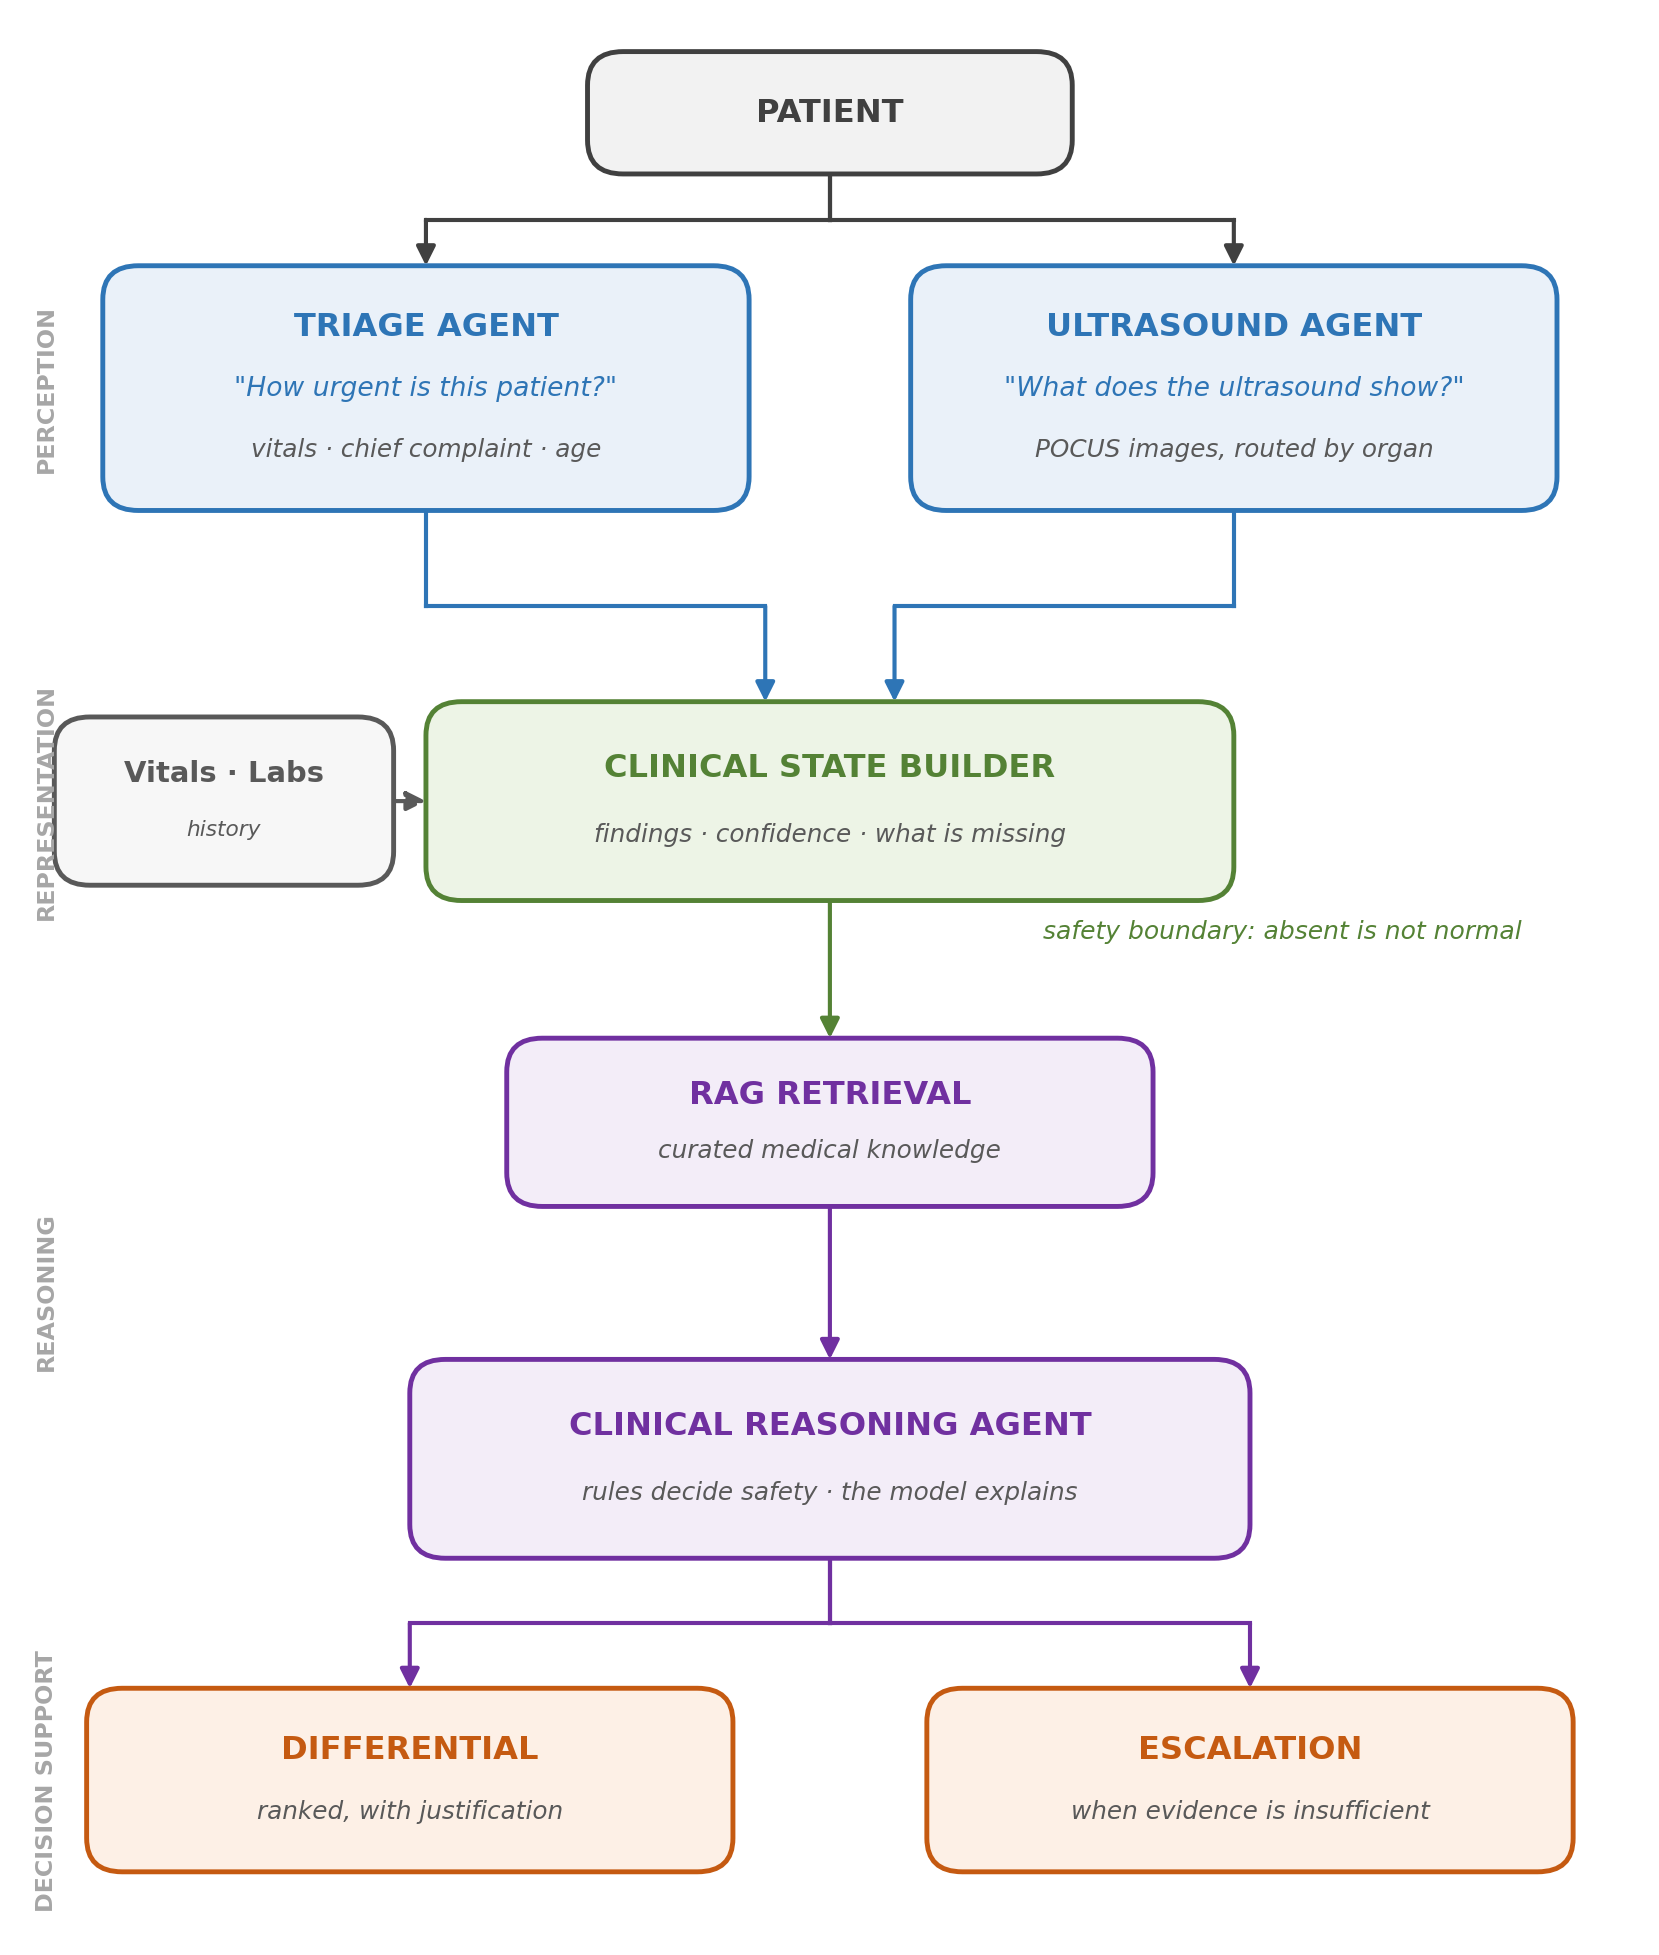
\includegraphics[width=0.70\textwidth]{fig_architecture.png}
  \caption{Overall architecture of POCUS-Emergency. Perception, representation, reasoning
    and decision support are separated into distinct layers. The Clinical State Builder
    acts as a safety boundary between the perception models and the language model.}
  \label{fig:architecture}
\end{figure}

Two perception agents operate in parallel. The \textbf{Triage Agent} focuses on the
patient rather than the image, estimating an urgency level from the chief complaint, vital
signs and age. The \textbf{Ultrasound Agent} focuses exclusively on \gls{pocus} data,
routing an examination to the appropriate organ-specific model and returning structured
findings with confidence information and Gradient-weighted Class Activation Mapping
(\gls{gradcam}) explanations. Its objective is not
to decide whether a patient is urgent, but to answer a more fundamental question: what
does the ultrasound show?

Their outputs are combined by the \textbf{Clinical Reasoning Agent}, which weighs them
against laboratory results and history while accounting for missing information, model
limitations and contradictions between sources. A retrieval-augmented generation
(\gls{rag}) mechanism grounds the reasoning in a curated medical knowledge base
\cite{lewis2020rag}, and a locally deployed
medical language model transforms the structured evidence into a ranked differential
diagnosis with supporting arguments, explicit uncertainty and an escalation decision.

\paragraph{Reasoning under uncertainty.} A further objective is to address uncertainty
explicitly rather than implicitly. In real emergency medicine, the absence of information
is not equivalent to a normal result. A laboratory test that was never performed cannot be
interpreted as negative, and a model that was never trained to detect a particular
pathology cannot be used to exclude it. The system therefore incorporates an intermediate
Clinical State Builder that standardises the outputs of the different agents and
represents explicitly the information that is available and the information that is
missing, the confidence attached to each finding and whether that confidence is
calibrated, the stated limitations of each model, and any conflict between clinical and
imaging evidence. This representation acts as a safety boundary: it prevents the reasoning
layer from silently treating missing evidence as negative evidence, or from interpreting a
model outside the scope it was trained for.

\subsection{Report Organization}
\label{subsec:organization}

The report follows the order in which the system was built, so that each chapter depends
only on what precedes it.

\begin{itemize}[label=$\bullet$]
  \setlength\itemsep{-0.1em}
  \item \textbf{Chapter~\ref{sec:environment} --- Project Environment and Presentation.}
    The host organisation, the context of the internship, the system architecture in
    detail, and the development methodology.
  \item \textbf{Chapter~\ref{sec:sota} --- Preliminary Study and State of the Art.}
    Existing work in automated ultrasound interpretation and multimodal decision support,
    its limitations, and the positioning of this project against it.
  \item \textbf{Chapter~\ref{sec:data} --- Datasets and Data Preparation.} The datasets
    used, their characteristics, and the determination of the statistical unit that
    governs every result reported afterwards.
  \item \textbf{Chapter~\ref{sec:perception} --- Perception Agents.} Development and
    evaluation of the triage, lung, cardiac and gallbladder modules, including the
    experiments that failed and the corrections they prompted.
  \item \textbf{Chapter~\ref{sec:reasoning} --- Clinical Reasoning Agent.} The clinical
    state representation, conflict detection, retrieval, the medical language model,
    output validation and the escalation policy.
  \item \textbf{Chapter~\ref{sec:integration} --- System Integration and Prototype.} The
    end-to-end pipeline, the contract through which the agents communicate, and worked
    clinical scenarios.
  \item \textbf{Chapter~\ref{sec:results} --- Results and Discussion.} The measured
    results for each module, what they mean clinically, and the limitations that remain.
  \item \textbf{Chapter~\ref{sec:conclusion} --- Conclusion and Perspectives.} The
    contributions, the objectives achieved, and directions for future work.
\end{itemize}

% =========================================================================================
% Chapter 2 -- Project Environment and Presentation
% =========================================================================================
\section{Project Environment and Presentation}
\label{sec:environment}

\subsection{Host Organization}
\label{subsec:host}

\rmq{Describe the host organisation: its activity, size, position in its sector, and the
department or team the internship took place in. Half a page to a page. If the project was
carried out within the school rather than a company, describe the laboratory or programme
instead.}

\subsection{Internship Environment}
\label{subsec:internship-env}

The project was carried out as an individual end-of-studies internship over a period of
three months, with the scope of a minimum viable product (\gls{mvp}) rather than a
deployable clinical product. All
design, implementation, experimentation and evaluation described in this report were
performed by the author, with periodic supervision and review.

The technical environment reflects that scope. Development was carried out in Python,
using PyTorch for the imaging models and scikit-learn together with XGBoost for the
structured-data model. Training was performed on Google Colab GPU instances, with local
execution reserved for data preparation, analysis and inference. \rmq{State the supervision
arrangement: frequency of meetings, review format, and any clinical input received.}

The intermittent availability of GPU hardware was a genuine constraint on the experimental
programme rather than an incidental inconvenience. It limited the number of training runs
that could be spent on any single question, and consequently shaped the methodology
described in Section~\ref{subsec:methodology}: candidate changes were, wherever possible,
estimated analytically from measurements already obtained before being committed to a
training run. This constraint is discussed further in Chapter~\ref{sec:conclusion}.

\subsection{Project Context}
\label{subsec:project-context}

The clinical problem was set out in Chapter~\ref{sec:introduction}: point-of-care
ultrasound is fast and available, but operator-dependent, and a single imaging finding
rarely determines a decision on its own. Existing automated approaches, reviewed in
Chapter~\ref{sec:sota}, address one organ and one question at a time.

The project therefore targets the layer above the individual model. Its contribution is
not a new segmentation architecture or a new classifier, but a system in which several
perception models cooperate with structured clinical data under an explicit account of
what each of them can and cannot support. That framing determines what counts as success:
a module is useful to this system when its output is accompanied by a trustworthy
statement of its own reliability, not merely when its headline metric is high.

\subsection{POCUS-Emergency}
\label{subsec:pocus-emergency}

POCUS-Emergency is a modular multi-agent assistant for emergency ultrasound and clinical
decision support. It accepts an ultrasound examination together with whatever structured
clinical data is available for the same patient, and returns a ranked differential
diagnosis, an explicit account of the uncertainty attached to it, and a decision on
whether the case should be escalated for further examination.

The system covers four perception modules --- triage, lung, cardiac and gallbladder ---
and the reasoning layer that combines them. A vascular / deep vein thrombosis (\gls{dvt})
module was considered
during planning and deliberately excluded from the scope of the internship, in order to
complete the four modules above to a defensible standard rather than five to a partial
one. The examination types the Ultrasound Agent does not support return an explicit
\textit{not supported} status rather than a low-confidence guess, for the reasons given in
Section~\ref{subsec:architecture}.

\subsection{System Architecture}
\label{subsec:architecture}

The system is organised as three agents with strictly separated responsibilities,
summarised in Tab.~\ref{tab:agents}. The separation is not incidental: it is the mechanism
by which the fourth difficulty of Section~\ref{subsec:problem} --- unwarranted confidence
--- is controlled.

\begin{table}[H]
  \centering
  \small
  \begin{tabularx}{\linewidth}{lXX}
    \toprule
    \textbf{Agent} & \textbf{Input} & \textbf{Output} \\
    \midrule
    Triage Agent & Chief complaint, vital signs, age, red-flag symptoms &
      Urgency level with calibrated confidence \\
    \addlinespace[2pt]
    Ultrasound Agent & Ultrasound image or clip, routed by organ &
      Findings with calibrated confidence and attention maps \\
    \addlinespace[2pt]
    Clinical Reasoning Agent & Both of the above, plus laboratory results and history &
      Ranked differential diagnosis and escalation decision \\
    \bottomrule
  \end{tabularx}
  \caption{Responsibilities of the three agents.}
  \label{tab:agents}
\end{table}

Each component rests on a distinct technology, and the report names them precisely rather
than describing the system uniformly as ``artificial intelligence''. Tab.~\ref{tab:tech}
gives the correspondence.

\begin{table}[H]
  \centering
  \small
  \begin{tabularx}{\linewidth}{lX}
    \toprule
    \textbf{Component} & \textbf{Technology} \\
    \midrule
    Triage Agent            & Gradient-boosted decision trees (XGBoost
                              \cite{chen2016xgboost}) with post-hoc probability
                              calibration \\
    Lung module             & \gls{cnn} classifier, multi-label, EfficientNet-B0 backbone
                              \cite{tan2019efficientnet} \\
    Cardiac module          & U-Net segmentation \cite{ronneberger2015unet} with an
                              EfficientNet-B0 encoder \\
    Gallbladder module      & \gls{cnn} classifier, EfficientNet-B0 backbone \\
    Explainability          & \gls{gradcam} \cite{selvaraju2017gradcam} \\
    Clinical state          & Deterministic Python; no model \\
    Knowledge grounding     & \gls{rag} over a curated corpus \cite{lewis2020rag} \\
    Differential reasoning  & Medical \gls{llm} \cite{chen2024huatuogpto1} \\
    Escalation              & Rule-based policy; deterministic \\
    \bottomrule
  \end{tabularx}
  \caption{Technology underlying each component of the system.}
  \label{tab:tech}
\end{table}

\subsubsection{Triage Agent}

The Triage Agent reads the patient record rather than the image. From the chief complaint,
vital signs, age and available red-flag indicators it estimates an urgency tier --- low,
medium or high --- together with a confidence. It operates on structured data only and
never sees an ultrasound image.

Two properties matter for the system as a whole. First, its confidence is calibrated, so
that a stated probability can be compared meaningfully against the confidence attached to
an imaging finding. Second, its output is deliberately coarse: three tiers rather than the
five-level scales used in hospital triage systems, because the reasoning layer uses the
tier to decide whether to escalate, not to assign a waiting time. The construction and
evaluation of this model are described in Section~\ref{subsec:triage-agent}.

\subsubsection{Ultrasound Agent}

The Ultrasound Agent is a router with organ-specific models behind it. Given an
examination and the organ examined, it dispatches the input to the corresponding module
and returns findings in a single shared output format, regardless of which module
produced them. Each finding carries a calibrated confidence, an indication of whether that
calibration was actually available, and a \gls{gradcam} map relating the prediction to
image regions the clinician can verify.

\begin{keystatement}
The Ultrasound Agent reports findings and does not assign urgency.
\end{keystatement}

This distinction is deliberate and is enforced throughout the implementation. A
radiologist records ``multiple B-lines, small consolidation, no pleural effusion''; the
inference to pulmonary oedema, and the decision about how urgently to act, require vital
signs, laboratory results and history that the imaging model never sees. Allowing an
imaging model to emit an urgency verdict would place a clinical decision inside a
component that lacks the information to make it, and would duplicate that logic in two
places within the system.

The same reasoning governs unsupported examinations. An organ for which no module was
built returns an explicit \textit{not supported} status in the ordinary output format,
rather than being silently omitted or answered with a low-confidence guess. A missing
module and a negative finding are different statements, and the reasoning layer must be
able to tell them apart.

\subsubsection{Clinical Reasoning Agent}

The Clinical Reasoning Agent occupies the position of the senior physician who receives
the nurse's rapid assessment and the imaging report, weighs both against the laboratory
results and the patient's history, and reaches a conclusion. It is the only component
permitted to decide urgency or recommend action.

\begin{keystatement}
A second separation applies within the reasoning agent itself: deterministic rules decide
what is safe, and the language model explains.
\end{keystatement}

The safety-critical determinations --- which tests are absent, which model limitations
apply, whether the agents disagree, whether escalation is warranted --- are computed by
deterministic rules before the language model is consulted, and the model's output is
checked against the structured state afterwards. The language model reasons over evidence
that has already been constrained; it does not decide whether the case is safe. Asking a
language model directly what should be done would place the least predictable component in
charge of the most consequential decision. This design is described in
Chapter~\ref{sec:reasoning}.

\subsection{Development Methodology}
\label{subsec:methodology}

\subsubsection{CRISP-DM and how it was adapted}

The project followed \gls{crisp}, the reference process model for data mining and data
science work. It was chosen over a software-engineering methodology because the central
risks here are not implementation risks. The difficulty in this project was rarely writing
the code; it was establishing what the data actually represented and whether a measured
result could be trusted. \gls{crisp} places those questions in named phases with explicit
feedback loops, which matches how the work behaved.

Tab.~\ref{tab:crispdm} states what each phase meant concretely here, and where the project
departed from the standard description.

\begin{table}[H]
  \centering
  \small
  \begin{tabularx}{\linewidth}{lXX}
    \toprule
    \textbf{Phase} & \textbf{In this project} & \textbf{Adaptation} \\
    \midrule
    Business Understanding & The four difficulties of
      Section~\ref{subsec:problem}; the Business and Data Science Objectives &
      Extended with an explicit safety requirement: a confident wrong answer is worse
      than no answer \\
    \addlinespace[2pt]
    Data Understanding & Provenance, acquisition characteristics, class distribution, and
      the statistical unit of each dataset &
      Far heavier than anticipated. The statistical unit was undocumented in every imaging
      dataset and had to be recovered \\
    \addlinespace[2pt]
    Data Preparation & Cleaning, taxonomy correction, preprocessing, and case-level
      grouping &
      Grouping is treated as a modelling decision, not a preprocessing step, because it
      determines what every later metric means \\
    \addlinespace[2pt]
    Modeling & The four perception modules and the reasoning layer &
      Split across two levels: individual models, and the contract through which they
      cooperate \\
    \addlinespace[2pt]
    Evaluation & Case-level metrics against baselines, calibration, error analysis and
      explainability &
      A calibration step was inserted between modelling and evaluation: the deliverable is
      not a prediction but a prediction with a trustworthy confidence \\
    \addlinespace[2pt]
    Deployment & --- &
      Out of scope for the internship. Replaced by integration and a prototype
      (Chapter~\ref{sec:integration}); no clinical deployment was undertaken \\
    \bottomrule
  \end{tabularx}
  \caption{The six CRISP-DM phases as applied in this project.}
  \label{tab:crispdm}
\end{table}

\begin{figure}[H]
  \centering
  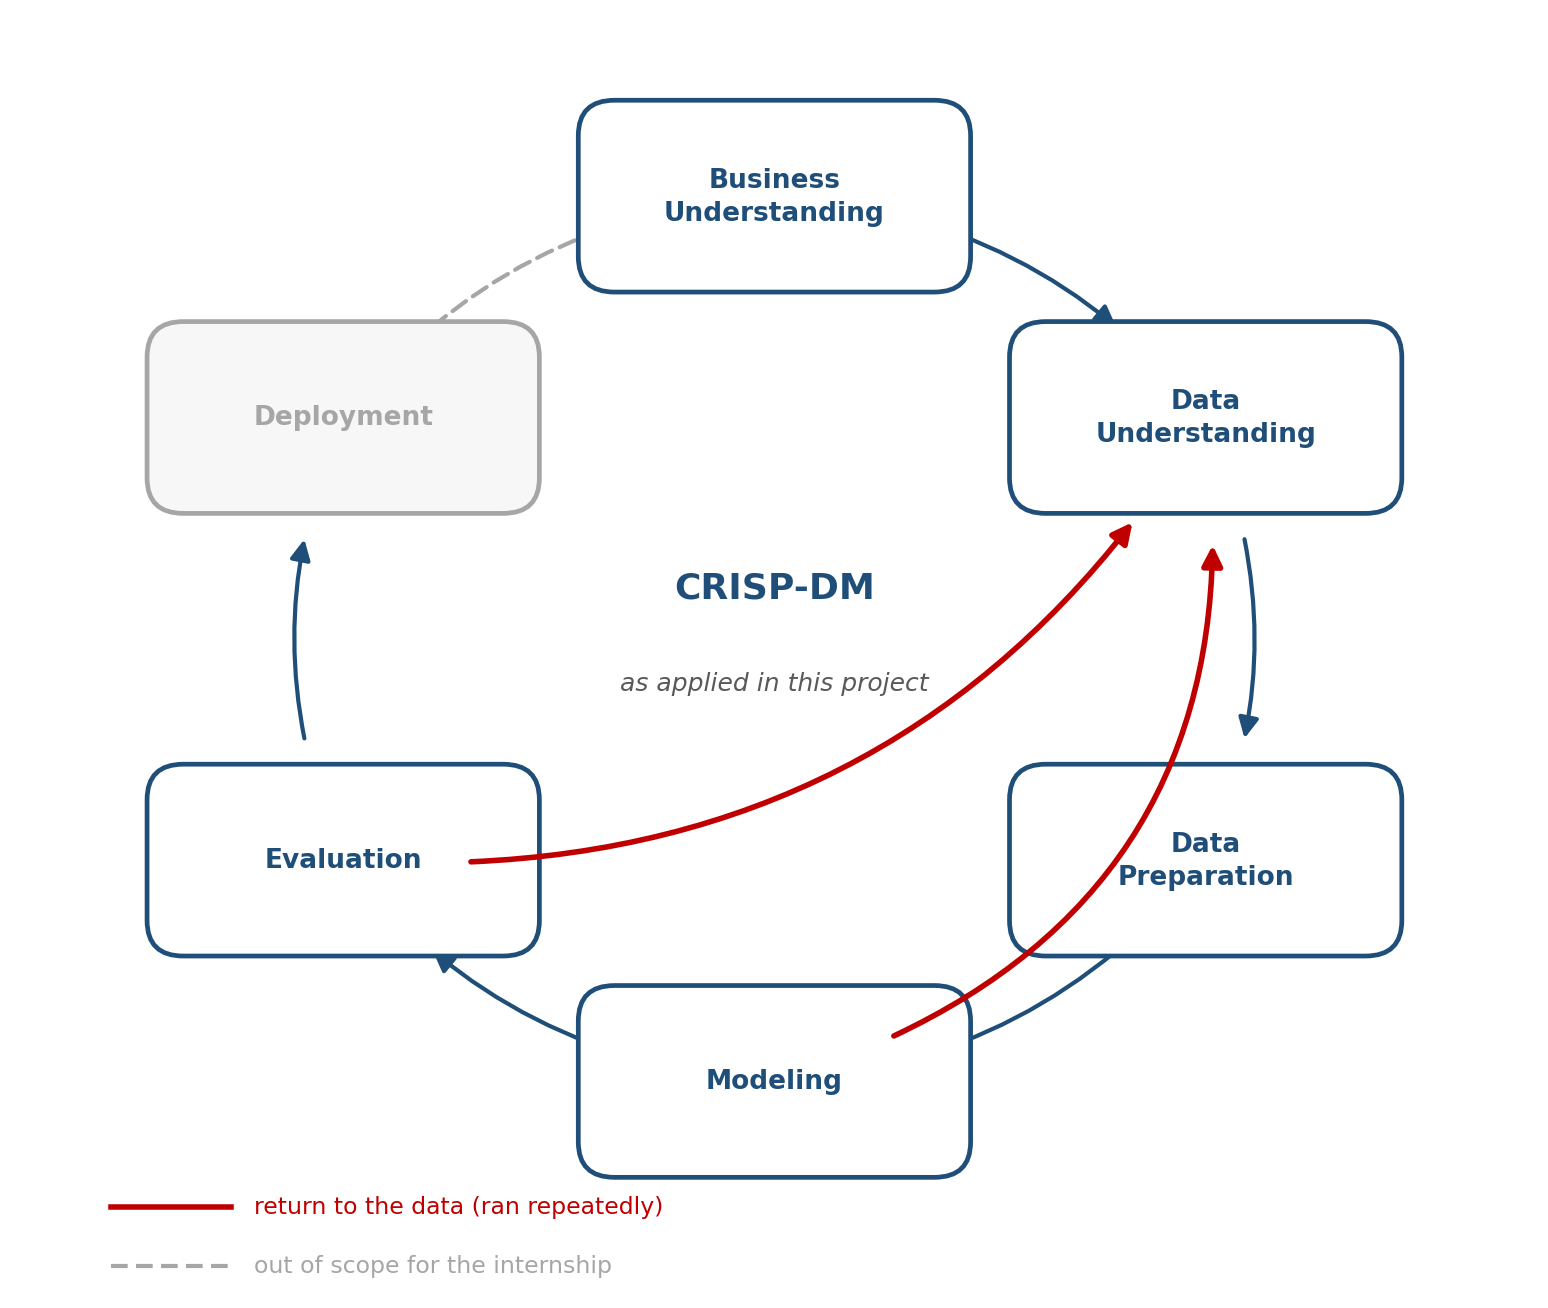
\includegraphics[width=0.72\textwidth]{fig_crispdm.png}
  \caption{The CRISP-DM cycle as followed here. The return path from modelling and
    evaluation to data understanding, drawn in red, ran repeatedly and was the dominant
    route through the cycle rather than an exception. Deployment was outside the scope of
    the internship.}
  \label{fig:crispdm}
\end{figure}

\paragraph{The loop back to the data was the main path, not an exception.} CRISP-DM allows
a return from Evaluation to earlier phases; in this project that return was where most of
the progress happened, and Fig.~\ref{fig:crispdm} draws it accordingly. Three times, a
model was trained and evaluated before the evaluation itself revealed that the data had
been misunderstood --- an unrecognised grouping structure in one dataset, a class whose
label did not match its images in another, an input feature that encoded the outcome in a
third. In each case the fix belonged to Data Understanding, not to Modeling, and the model
had to be discarded and retrained. A linear reading of the process would have concluded
after the first evaluation and reported a number that could not be defended.

\subsubsection{Development phases}

The work was organised into sequential phases, each concluding with a working, evaluated
component. The ordering was chosen so that every phase produced something the next phase
depended on, rather than developing components in parallel and integrating them at the
end. The phases are listed in Tab.~\ref{tab:phases}.

\begin{table}[H]
  \centering
  \small
  \begin{tabularx}{\linewidth}{clXl}
    \toprule
    \textbf{Phase} & \textbf{Objective} & \textbf{Outcome} & \textbf{Status} \\
    \midrule
    1 & Triage Agent & Three-tier urgency classifier (low / medium / high), calibrated
      & Complete \\
    \addlinespace[2pt]
    2 & Perception modules & Lung, cardiac and gallbladder models with calibrated
      confidence & Complete \\
    \addlinespace[2pt]
    3 & Unified Ultrasound Agent & Organ routing, shared output contract, encounter
      storage & Complete \\
    \addlinespace[2pt]
    4 & Clinical State Builder & Standardised representation of all agent outputs
      & Complete \\
    \addlinespace[2pt]
    5 & Clinical Reasoning Agent & Safety layer, escalation policy, retrieval and
      reasoning & In progress \\
    \bottomrule
  \end{tabularx}
  \caption{Development phases of the project.}
  \label{tab:phases}
\end{table}

\subsubsection{Methodological rules}

\paragraph{One methodological rule governed all phases.} No design decision was adopted on
the basis of expectation alone. Where a change was proposed --- a different architecture,
an augmentation strategy, an additional dataset --- it was implemented, measured against
the existing baseline, and retained only if the measurement supported it.

Several proposals that appeared well motivated were rejected on this basis, and those
rejections are reported in the chapters that follow rather than omitted. They are, in
several cases, more informative than the successes: a change that ought to have helped and
did not tells the reader something about the data that a favourable number does not. In a
clinical context, a result that cannot be defended is of no use regardless of how
favourable it appears.

\paragraph{Reporting convention.} Throughout Chapters~\ref{sec:perception}
and~\ref{sec:results}, three distinct statements are kept separate: what was
\textit{built}, what was \textit{measured}, and what may reasonably be \textit{concluded}.
A model architecture is a construction; a Dice coefficient on a held-out partition is a
measurement; a statement about how the model will behave on data from another hospital is
a conclusion, and requires more than the measurement to support it. Conflating the three
is the most common way a report overstates its results, and it is avoided here
deliberately.


\part{CRISP-DM}
% =========================================================================================
% Chapter 3 -- Preliminary Study and State of the Art
% =========================================================================================
\section{Preliminary Study and State of the Art}
\label{sec:sota}

\subsection{Introduction}

This chapter reviews the work this project builds on and measures itself against. It moves
from the clinical setting to the technical one: what point-of-care ultrasound is used for
in emergency medicine, why automated interpretation of ultrasound is harder than of other
imaging modalities, what has been published on the specific organs addressed here, and what
exists in multimodal clinical decision support. It closes by stating the limitations that
recur across this literature and the position this project takes with respect to them.

\subsection{POCUS in Emergency Medicine}
\label{subsec:sota-pocus}

Point-of-care ultrasound differs from radiological ultrasound in who performs it and why.
It is performed by the treating clinician, at the bedside, to answer a specific binary
question arising from the patient in front of them --- is there fluid in the abdomen, is
the left ventricle contracting, is this dyspnoea cardiogenic --- rather than to produce a
comprehensive report.

That framing has produced a set of standardised protocols. The BLUE protocol
\cite{lichtenstein2008blue} reduces the diagnosis of acute respiratory failure to a short
sequence of chest views, each with a defined interpretation, and reports high diagnostic
accuracy for the principal causes of dyspnoea. The \gls{fast} examination applies the same
logic to injury, searching four windows for free fluid. Focused echocardiography in
undifferentiated shock follows a comparable structure.

Two properties of these protocols matter for what follows. First, they are defined in terms
of \emph{findings} rather than diagnoses: the operator records whether B-lines are present,
not whether the patient has heart failure. Second, they are explicitly bounded --- each
protocol states which questions it answers and, by omission, which it does not. Both
properties are adopted directly by the Ultrasound Agent described in
Section~\ref{subsec:ultrasound-agent}.

\paragraph{Operator dependence is measurable, and larger than is often assumed.} The
systematic review by Andersen et al.\ \cite{andersen2019pocus} quantifies it across
applications. False-positive rates varied from 0.7\% to 33.3\% depending on the type of
examination: 0.7--3.2\% for obstetric scans, 0.5--9.9\% for abdominal, and 4.0--33.3\% for
cardiac. A spread of that magnitude within a single application is the empirical form of
the problem stated in Section~\ref{subsec:problem}.

Reported training volumes vary equally widely --- from 2.3 to 31 hours for focused scans,
and from 4 to as much as 320 hours for multi-anatomical examinations. The review's most
useful finding, however, is a negative one: it identified no overall association between
the amount of training and diagnostic accuracy. What determined accuracy was the type of
examination rather than the hours logged, with focused scans outperforming comprehensive
ones, and competence in some applications reached after only a few hours.

That result points the same way as the protocol design discussed above, and it has a direct
architectural consequence here. A bounded question asked of a single organ is answered
reliably; an open-ended examination is not. It is the reason the Ultrasound Agent is built
as a set of narrow per-organ modules, each declaring what it does and does not cover,
rather than as one general-purpose interpreter of ultrasound.

One qualification should be stated with these figures. The review covers general practice
rather than emergency medicine, and the two settings differ in case mix, in operator
training and in the urgency under which examinations are performed. The mechanism ---
accuracy governed by the boundedness of the question asked --- transfers; the specific
percentages should not be read as emergency-department values.

\subsection{AI for Medical Ultrasound}
\label{subsec:sota-ai-us}

Ultrasound is a harder target for computer vision than computed tomography or magnetic
resonance imaging, for reasons intrinsic to the modality rather than incidental to it.

\paragraph{The image depends on the operator.} A CT volume of a given patient is
essentially reproducible; an ultrasound image is a function of probe position, angle,
pressure, depth setting, gain and patient habitus. Two competent operators produce visibly
different images of the same anatomy, so a model must be robust to a source of variation
that barely exists in other modalities.

\paragraph{Speckle is signal and noise at once.} The granular texture of ultrasound arises
from interference of the returning wave. It is not additive noise that can be filtered away
without loss, and conventional denoising removes diagnostic information along with it.

\paragraph{Several findings are artefacts, not anatomy.} This is the property most often
overlooked. \gls{blines} and \gls{alines} do not correspond to structures in the lung; they
are reverberation artefacts whose presence and distribution carry the diagnostic meaning
\cite{lichtenstein2008blue}. A model trained to segment anatomy is solving the wrong problem
for lung ultrasound, which is why the lung module in this project is a classifier and the
cardiac module is a segmentation network.

\paragraph{There is no canonical orientation.} Manufacturers and operators differ in how the
image is presented, and public datasets inherit those differences without documenting them.
This bears directly on the external-validation gap reported in
Section~\ref{subsec:cardiac-results}.

\subsection{Ultrasound Segmentation and Classification}
\label{subsec:sota-seg-cls}

Two task families cover the work in this project.

\emph{Segmentation} assigns a label to every pixel, and is the appropriate formulation when
the clinical quantity is geometric --- a chamber area, a volume, an ejection fraction. The
encoder--decoder architecture introduced by U-Net \cite{ronneberger2015unet}, in which
skip connections carry high-resolution detail across the bottleneck, remains the basis of
most medical segmentation work. Modern variants typically substitute a stronger pretrained
encoder, such as EfficientNet \cite{tan2019efficientnet}, while keeping the overall shape.

\emph{Classification} assigns labels to a whole image or clip, and is appropriate when the
clinical question is about presence rather than extent. It divides further into
single-label problems, where classes are mutually exclusive, and multi-label problems,
where they are not. The distinction is not cosmetic: a lung clip may show B-lines and
consolidation simultaneously, so the lung module must emit independent probabilities per
finding rather than a distribution over one categorical variable.

\paragraph{A methodological caveat that recurs throughout this literature.} Many published
results report metrics computed over frames or images. Where several frames originate from
one patient or one acquisition, a partition drawn at frame level places near-duplicates on
both sides of it, and the resulting score measures memorisation as much as generalisation.
Such figures are not directly comparable with case-level results. This is treated at length
in Chapter~\ref{sec:data}, because it governs the interpretation of every number reported
in this report.

\subsection{Existing POCUS AI Approaches}
\label{subsec:sota-existing}

\subsubsection{nnU-Net and the CAMUS benchmark}

The \gls{camus} dataset \cite{leclerc2019camus} is the reference resource for cardiac
ultrasound segmentation. It comprises 1{,}000 two-dimensional sequences --- two-chamber and
four-chamber views from 500 patients --- with expert contours of the left ventricular
endocardium, the epicardium and the left atrium at the end-diastolic and end-systolic
instants. Crucially for this project, its patient structure is explicit, which is what
makes correct grouping possible without reconstruction.

The accompanying study established that encoder--decoder architectures of the U-Net family
outperform earlier methods and reach accuracy within expert variability. The dataset is
maintained as an open challenge, and the current leaderboard provides the benchmark against
which the cardiac module of this project is measured. Tab.~\ref{tab:camus} reproduces the
leading entry alongside the intra-observer variability recorded for the reference contours.

\begin{table}[H]
  \centering
  \small
  \begin{tabular}{lcccc}
    \toprule
    & \multicolumn{2}{c}{\textbf{Best reported}} &
      \multicolumn{2}{c}{\textbf{Intra-observer}} \\
    \cmidrule(lr){2-3}\cmidrule(lr){4-5}
    \textbf{Structure} & ED & ES & ED & ES \\
    \midrule
    LV endocardium & 0.952 & 0.935 & 0.945 & 0.930 \\
    LV epicardium  & 0.963 & 0.959 & 0.957 & 0.951 \\
    Left atrium    & 0.902 & 0.935 & --- & --- \\
    \bottomrule
  \end{tabular}
  \caption{Dice coefficients on the CAMUS challenge leaderboard, for the leading
    nnU-Net-based entry, with the intra-observer variability of the reference contours for
    comparison. No intra-observer figure is published for the left atrium.}
  \label{tab:camus}
\end{table}

Two observations matter for later chapters. The leading automated results now equal or
exceed intra-observer agreement on both ventricular structures, so the remaining headroom
on this dataset is small. And performance is consistently lower on the left atrium and on
low-quality or artefact-heavy images --- a pattern the cardiac module of this project
reproduces, and which is discussed in Section~\ref{subsec:cardiac-results}.

nnU-Net \cite{isensee2021nnunet} approaches the problem differently, configuring
preprocessing, architecture and training schedule automatically from properties of the
dataset. Its relevance here is as a benchmark rather than a component: it defines the
performance a well-configured standard pipeline achieves on this data, and the cardiac
results in Section~\ref{subsec:cardiac-results} are reported against it.

\subsubsection{USCL: contrastive pretraining on ultrasound}

Most ultrasound models initialise from ImageNet weights, despite natural photographs
sharing little with speckle texture. USCL \cite{chen2021uscl} addresses this directly,
pretraining on ultrasound video through semi-supervised contrastive learning. The authors
assembled US-4, comprising over 23{,}000 images from four ultrasound video sub-datasets,
and report that a USCL-pretrained backbone reaches over 94\% fine-tuning accuracy on the
POCUS lung dataset against 84\% for ImageNet initialisation.

The motivation is sound and the reported gain is substantial, which is why this project
evaluated it. The measurement obtained here disagreed: on the gallbladder task, USCL
initialisation performed markedly worse than ImageNet initialisation. That result is
reported in Section~\ref{subsec:results-rejected} with its numbers. It is not presented as
a refutation of the original work --- the published claim concerns lung classification on
the dataset the pretraining corpus was drawn from, whereas the task here was multi-class
gallbladder classification on a small number of cases --- but it is the reason the
technique was not adopted, and the discrepancy is stated rather than omitted.

\subsubsection{Auto-US: an ultrasound video diagnosis agent}

Auto-US \cite{yang2025autous} is the closest published work to the present project and
deserves detailed comparison. It is described by its authors as the first agent combining
deep learning with \glspl{llm} for ultrasound video-assisted diagnosis, and is organised
into three stages --- video perception, clinical reasoning and diagnostic decision-making
--- which parallel the perception, representation and reasoning layers of
Fig.~\ref{fig:architecture}.

Its perception component, CTU-Net, is a CNN--Transformer network exploiting temporal,
spatial and frequency information in ultrasound video. It is evaluated on the CUV dataset,
assembled by the authors from open-access sources: 495 videos spanning five disease
categories across three organs. The reported classification accuracy is 86.73\%, and
clinician ratings of the generated diagnostic text exceed 3 out of 5.

The convergence is notable: two independent efforts arrived at the same decomposition of
perception followed by language-model reasoning. The differences are equally instructive
and define where this project contributes.

Auto-US pairs ultrasound video with clinical \emph{text} --- chief complaint, physical
examination and additional information --- rather than with structured measurements. Vital
signs and laboratory values are not among its inputs. The paper reports no confidence
calibration or uncertainty quantification for its predictions, no explicit representation
of missing or unmeasured data, and no mechanism for resolving disagreement between the
video classifier and the language model's reasoning. Those four mechanisms are precisely
what this project treats as central, which places its contribution alongside Auto-US rather
than in competition with it.

The authors themselves make the case for going further, observing that ``relying solely on
ultrasound imaging is insufficient for obtaining accurate diagnostic opinions''
\cite{yang2025autous}. Extending that observation from clinical text to vital signs and
laboratory results, and adding an explicit account of what the models cannot exclude, is
the step taken here.

\subsubsection{The POCUS lung ultrasound dataset}

The lung module uses the public dataset released by Born et al.
\cite{born2021pocus}. It comprises 202 videos and 59 images acquired with convex and linear
probes from 216 patients, covering COVID-19, bacterial pneumonia, non-COVID viral
pneumonia and healthy controls, aggregated from heterogeneous sources.

Its strengths and weaknesses both follow from that construction. The heterogeneity is
representative of real point-of-care acquisition, which is desirable. But provenance is
mixed, acquisition is uncontrolled, and --- decisively for this project --- the release
carries no patient identifier linking the multiple clips belonging to one patient. Case
identity therefore has to be reconstructed before any honest partition can be drawn, which
is the subject of Section~\ref{subsec:data-grouping}. \rmq{The dataset has a published
erratum; check which version the downloaded copy corresponds to and cite accordingly.}

\subsection{Multimodal Clinical Decision Support}
\label{subsec:sota-multimodal}

Combining imaging with the rest of the clinical record is the problem this project is
ultimately about, and it has been studied independently of ultrasound. The systematic
review by Huang et al.\ \cite{huang2020fusion} surveys deep-learning systems that fuse
medical imaging with electronic health record data and provides the vocabulary used here.

It distinguishes three strategies. \emph{Early fusion} concatenates the input modalities
into a single feature vector before any model sees them. \emph{Joint fusion} combines
learned intermediate representations, with the loss propagated back into each
modality-specific encoder during training. \emph{Late fusion} trains a separate model per
modality and aggregates their predictions afterwards.

Two of the review's findings matter for the design adopted here. The first is that fusion
works: across the studies surveyed, multimodal models improved accuracy by 1.2--27.7\% and
AUROC by 0.02--0.16 over single-modality baselines, though no single fusion strategy was
consistently optimal across domains. The second is a distributional observation --- of the
17 studies reviewed, 11 (65\%) used early fusion and only 3 (18\%) used late fusion. The
field's default is to fuse early, inside one model.

\paragraph{The property that decides the question for an emergency system.} The same review
notes that late fusion is uniquely able to produce a prediction when not all modalities are
present, because each modality has its own model and the aggregation step can operate over
whichever predictions exist. Early and joint fusion architectures expect a complete input
vector, and have no defined behaviour when part of it is absent.

For a system evaluating an emergency patient this is not a secondary consideration. Missing
data is the normal condition, not the exception: the troponin has not come back, the
history is unobtainable, no ultrasound of that organ was performed. An architecture whose
behaviour is undefined when a modality is missing is undefined most of the time.

The evidence that late fusion also performs competitively is direct. In a case study on
pulmonary embolism detection from CT together with EHR data, Huang et al.\
\cite{huang2020pe} report a late-fusion model reaching an AUROC of 0.947, exceeding the
EHR-only model by 0.036 and the imaging-only model by 0.156. Late fusion was the
best-performing strategy tested, not a concession made for the sake of robustness.

\paragraph{Where this project goes further, and on what basis.} The architecture described
in Section~\ref{subsec:architecture} is late fusion in the sense above --- separate models
per modality, combined afterwards --- but the combination is not an aggregation function
over probabilities. The perception outputs are written into a structured clinical state
that records confidence, evidence grade, model scope and what was not measured, and a
reasoning layer consumes that state.

The motivation is attribution. Under early or joint fusion a single confidence emerges from
the combined model, and a clinician reading it cannot tell whether the imaging or the vital
signs produced it; under the design used here, each finding retains the confidence of the
module that produced it, and disagreement between modules remains visible instead of being
averaged away.

This last point is offered as a design argument rather than as an established result. The
systematic review cited above does not compare fusion strategies with respect to
interpretability, and no measurement in this project isolates the benefit of attribution
from the other properties of the architecture. It is a reason for the design, not evidence
for it.

\subsection{Large Language Models and Retrieval-Augmented Generation}
\label{subsec:sota-llm}

Large language models can integrate heterogeneous evidence and produce structured reasoning
over it, which is the capability the reasoning layer of this system requires. Domain-adapted
medical reasoning models such as HuatuoGPT-o1 \cite{chen2024huatuogpto1} extend this to
clinical material specifically.

Retrieval-augmented generation \cite{lewis2020rag} supplies a model with passages retrieved
from a trusted corpus at inference time, so that its output is grounded in citable sources
rather than in its parameters alone. For clinical use the attraction is less the additional
knowledge than the traceability: an assertion accompanied by the passage it came from can be
checked.

\paragraph{The failure mode that motivates the safety layer.} A fluent model asked to reason
about a patient will produce a fluent answer whether or not the evidence supports one. Left
unconstrained it will cite a laboratory value that was never measured, or treat the absence
of a finding as evidence of health. Retrieval reduces but does not eliminate this: it
grounds the general knowledge while leaving the patient-specific assertions ungrounded.
Neither retrieval nor domain adaptation constitutes a guarantee, which is why in this
project the safety-critical determinations are computed deterministically and the model's
output is validated against the structured state afterwards
(Chapter~\ref{sec:reasoning}).

\subsection{Limitations of Existing Approaches}
\label{subsec:sota-limits}

Five limitations recur across the work reviewed above. They are stated as properties of the
literature, not as criticism of individual papers, most of which address a narrower question
than the one posed here.

\begin{enumerate}
  \setlength\itemsep{0.25em}
  \item \textbf{One organ, one question.} Models are developed and evaluated on a single
    organ. An undifferentiated emergency patient does not present a single question, and
    nothing in these systems combines their outputs.
  \item \textbf{Evaluation below the level of the patient.} Metrics are frequently computed
    over frames or images, inflating measured performance wherever several derive from one
    patient.
  \item \textbf{Uncalibrated confidence reported as probability.} A softmax output is
    routinely presented as a probability without being checked against observed frequency
    \cite{guo2017calibration}. A clinician reading 0.8 as ``correct four times in five''
    is entitled to be wrong.
  \item \textbf{No representation of absent evidence.} A test never performed and a test
    returning normal are distinct states, and systems that lack the distinction implicitly
    treat the first as the second.
  \item \textbf{No defined behaviour when sources disagree.} Where multiple signals are
    available, disagreement is typically resolved by whichever model is more confident,
    rather than being surfaced as the clinically important event it is.
\end{enumerate}

\subsection{Positioning of Our Approach}
\label{subsec:sota-positioning}

\begin{keystatement}
The individual models in this project are standard architectures and are not claimed as
contributions. The contribution is the layer above them.
\end{keystatement}

The cardiac module is a U-Net with an EfficientNet encoder; the lung and gallbladder
modules are EfficientNet classifiers; the triage model is gradient-boosted trees. Each was
selected because it is a defensible standard choice for its task, not because it is novel,
and Chapter~\ref{sec:results} reports them against published benchmarks rather than
claiming to advance them.

What this project adds is the structure in which they cooperate, addressing the five
limitations above in order: a shared output contract across four modules covering both
imaging and structured data; case-level evaluation throughout; a calibrated confidence per
module, carried through to the reasoning step rather than discarded at the module boundary;
an explicit representation of what was not measured and what each model cannot exclude; and
a deterministic policy that escalates on disagreement instead of resolving it.

Tab.~\ref{tab:positioning} sets this against the work reviewed in this chapter. It compares
\emph{capabilities rather than performance}, and the distinction is deliberate. The systems
reviewed here address different organs, different tasks and different datasets: a Dice
coefficient for cardiac segmentation, a classification accuracy on ultrasound video and a
balanced accuracy on gallbladder cases are not commensurable quantities, and placing them in
a single column would invite a comparison that none of them supports. Measured performance
is reported in Chapter~\ref{sec:results}, where each module is compared against its own
baseline and against the benchmark for its own task.

The table should therefore be read across the rows: \emph{yes} indicates that a system
provides the mechanism, \emph{no} that it is a system which does not, and \emph{n/a} that
the contribution is a dataset, benchmark or training method to which the question does not
apply. The bottom row is the only one carrying \emph{yes} in every column, and that is the
claim this project makes --- not that its models are more accurate than the published ones,
but that they are assembled into a system that knows what it does not know.

\begin{table}[H]
  \centering
  \small
  \setlength{\tabcolsep}{4pt}
  \begin{tabular}{llccccc}
    \toprule
    \textbf{Work} & \textbf{Type} & \textbf{Organs} & \textbf{Non-imaging} &
    \textbf{Calibrated} & \textbf{Absent} & \textbf{Conflict} \\
    & & & \textbf{inputs} & \textbf{confidence} & \textbf{evidence} & \textbf{policy} \\
    \midrule
    CAMUS / nnU-Net \cite{leclerc2019camus, isensee2021nnunet}
      & benchmark   & 1 & none & n/a & n/a & n/a \\
    USCL \cite{chen2021uscl}
      & pretraining & 1 & none & n/a & n/a & n/a \\
    POCUS lung \cite{born2021pocus}
      & dataset     & 1 & none & n/a & n/a & n/a \\
    Auto-US \cite{yang2025autous}
      & agent       & 3 & clinical text & no & no & no \\
    \addlinespace[3pt]
    \textbf{This work}
      & agent       & 3 + triage & vitals, labs & yes & yes & yes \\
    \bottomrule
  \end{tabular}
  \caption{Positioning against the reviewed work. ``n/a'' marks a mechanism that does not
    apply to the kind of contribution: a dataset or a pretraining method is not expected to
    provide a conflict policy. Only Auto-US and the present work are complete systems, and
    only those two rows are directly comparable.}
  \label{tab:positioning}
\end{table}

\subsection{Conclusion}

The literature provides strong single-organ models, a reference benchmark for cardiac
segmentation, public data for lung ultrasound, and --- in Auto-US --- an independent
confirmation that perception followed by language-model reasoning is a reasonable
decomposition. What it does not provide is a system that combines imaging with the rest of
the emergency record while keeping an honest account of its own reliability.

The next chapter turns to the data, and to the question that had to be answered before any
model could be trained: what a single independent observation actually is in each of these
datasets.

% =========================================================================================
% Chapter 4 -- Data Understanding (CRISP-DM)
%
% All counts here were read from the manifests, not from notes. Regenerate with
% scratchpad/dataset_facts.py and dataset_facts2.py if the manifests change.
% =========================================================================================
\section{Data Understanding}
\label{sec:data}

\subsection{Introduction}

This chapter describes the data the four perception modules were built on, and the single
question that had to be answered before any of them could be trained honestly: what counts
as one independent observation.

The question sounds procedural. It is not. Answering it wrongly inflates every metric that
follows, and does so invisibly --- the model appears to work, the validation score confirms
it, and nothing in the training process signals a problem. In each of the three imaging
datasets used here, the answer was not the one the file listing suggested.

\subsection{Dataset Overview}
\label{subsec:data-overview}

Four datasets were used, one per module. Tab.~\ref{tab:datasets} gives their composition.

\begin{table}[H]
  \centering
  \small
  \setlength{\tabcolsep}{5pt}
  \begin{tabular}{llrrl}
    \toprule
    \textbf{Module} & \textbf{Source} & \textbf{Files} & \textbf{Cases} &
    \textbf{Label type} \\
    \midrule
    Triage      & Four pooled ED datasets            & 164{,}700 & 164{,}700 &
      urgency tier (3) \\
    Cardiac     & CAMUS \cite{leclerc2019camus}      & 2{,}000 & 500 &
      pixel masks (3 structures) \\
    Gallbladder & UIdataGB (Mendeley)                & 10{,}694 & 220 &
      pathology class (9) \\
    Lung        & POCUS \cite{born2021pocus}         & 187 & 165 &
      findings (4, multi-label) \\
    \bottomrule
  \end{tabular}
  \caption{Composition of the four datasets. For the imaging datasets, ``files'' counts
    images, annotated frames or clips, and ``cases'' counts independent patients or
    acquisitions. The gap between the two columns is the subject of
    Section~\ref{subsec:data-grouping}.}
  \label{tab:datasets}
\end{table}

All four sources are publicly available and were obtained free of charge for academic
research. Their terms are not uniform, and the differences shaped how the project stores data.

The lung dataset \cite{born2021pocus} is a collection of contributions rather than a single
release, and the licence varies by contributing source: material from Neuruppin is CC~BY~4.0,
material from Northumbria is CC~BY--NC~4.0, and some items the original study used could not
be redistributed in its own repository at all. The cardiac dataset (CAMUS
\cite{leclerc2019camus}) and the gallbladder dataset (UIdataGB, Mendeley Data) are released
for research use. The triage sources are public-use files: NHAMCS is a United States federal
public-use release, the Iran ED data accompanies an open-access publication, and MC-MED and
MIMIC-IV-ED were used in their public demonstration releases, the credentialed full versions
being outside the scope of this work.

Two consequences follow, and both are visible in the deliverables. No source permits
wholesale redistribution of the media, so this project's repository contains
\emph{manifests} --- the lists of rows used, with their exclusion flags --- rather than
images, and reproduction requires obtaining the sources from their original providers. And
because several sources are non-commercial, the work reported here is academic; any use
beyond that would require re-examining each licence individually rather than treating the
collection as one permission.

\subsection{The Statistical Unit}
\label{subsec:data-grouping}

\begin{keystatement}
The gallbladder dataset contains 10{,}694 images. It does not contain 10{,}694 patients. It
contains 220.
\end{keystatement}

Medical imaging datasets are distributed as collections of files, and it is natural to treat
each file as one observation. For these datasets that is wrong, because the files are not
independent of one another. A single gallbladder examination contributed a median of 48
images --- and in one case 228 --- taken seconds apart, of the same organ, in the same
patient, under the same machine settings. Two such images are close to duplicates.

The consequence is specific. If a partition into training and validation data is drawn over
files, images from one examination land on both sides of it. The model then encounters, at
validation time, near-copies of images it memorised during training. It scores well. The
score measures recall of the training set, not generalisation to a new patient, and no
diagnostic within the training process distinguishes the two.

Fig.~\ref{fig:filesvscases} shows the size of the effect across the three imaging datasets.

\begin{figure}[H]
  \centering
  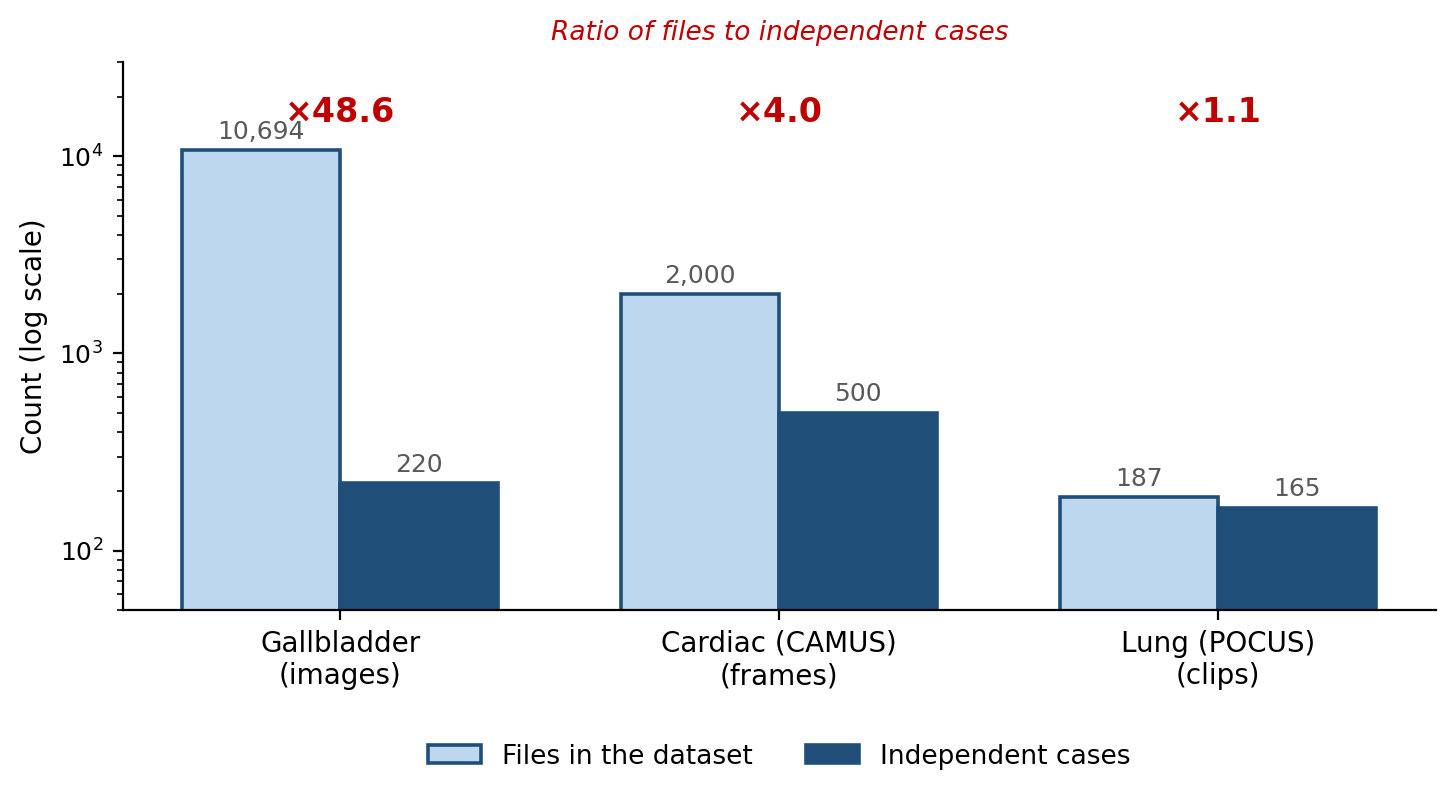
\includegraphics[width=0.86\textwidth]{fig_files_vs_cases.png}
  \caption{Files against independent cases for the three imaging datasets. The ratio bounds
    how far a file-level evaluation can overstate performance: the gallbladder dataset
    offers roughly 48 near-duplicate images per case, the cardiac dataset four annotated
    frames per patient, and the lung dataset only marginally more clips than patients.}
  \label{fig:filesvscases}
\end{figure}

The three datasets differ in how exposed they are. The lung dataset is nearly safe at
\(\times 1.1\); the cardiac dataset is moderately exposed at \(\times 4\); the gallbladder
dataset, at \(\times 48.6\), is where a file-level split would have produced a result with
no meaning at all.

\subsection{Recovering Case Identity}
\label{subsec:data-cases}

Knowing that the case is the unit is only useful if cases can be identified. The three
datasets required three different amounts of work.

\paragraph{Cardiac --- documented.} CAMUS is organised by patient. Each of the 500 patients
contributes two views (two-chamber and four-chamber), each annotated at end-diastole and
end-systole, giving 2{,}000 annotated frames. The grouping is read directly from the
directory structure and needs no reconstruction.

\paragraph{Gallbladder --- recoverable.} Case identity is not a column in the release, but
it is encoded in the filenames, which carry a per-case prefix. Parsing it yields 220 cases
across nine classes, with between 6 and 228 images each.

\paragraph{Lung --- reconstructed, with residual uncertainty.} The POCUS release carries no
patient identifier at all, while containing several clips of the same patient. Case identity
had to be inferred from filename patterns: explicit case numbers where present, day-series
markers for repeat examinations of one patient, and clip-numbering suffixes otherwise, with
a list of generic tokens excluded so that words such as \textit{video} or \textit{butterfly}
are not mistaken for patient identifiers. This recovered 165 cases from 187 files, with six
cases contributing more than one file and the largest contributing eight.

\begin{keystatement}
This last mapping is a heuristic, not ground truth. It is reported as such.
\end{keystatement}

Two clips of the same patient under different filename conventions may still be counted as
two cases, which would leave a small amount of leakage in place. The direction of that error
is known --- it can only inflate the lung results, never deflate them --- and it is carried
forward as a stated limitation rather than presented as a solved problem.

% =========================================================================================
% Chapter 5 -- Data Preparation (CRISP-DM)
%
% Split out of the former combined data chapter. The cut point is deliberate: this file
% begins where the description of the data ends and the operations on it begin. No
% paragraph was reordered in the split.
% =========================================================================================
\section{Data Preparation}
\label{sec:dataprep}

\subsection{Introduction}

Chapter~\ref{sec:data} established what these datasets contain and what counts as one
independent observation in each. This chapter describes what was then done to them: the
exclusions applied, the distributions that remained afterwards, the baselines those
distributions imply, and the partitioning that keeps a case on one side of the split.

The order matters. Every count reported here is a count after exclusion, and every baseline
is computed on the partition the module is actually evaluated on rather than on the pooled
data --- which is why they appear after the cleaning that produced them and not before.

\subsection{Cleaning and Exclusions}
\label{subsec:data-cleaning}

\paragraph{Lung.} Eleven files were excluded as off-target (not showing lung) and one as
flagged unusable by the dataset curators, reducing 198 files to the 187 used.

\paragraph{Gallbladder.} One class was found, on inspection, not to match its label. The
error is worth recording because of how it was made rather than merely that it occurred: the
class was first judged from a handful of images and appeared unremarkable. Viewing one image
per case, across all cases, showed otherwise.

\begin{keystatement}
Images from one case are not a sample of a class. They are a sample of a patient.
\end{keystatement}

The rule generalises beyond this incident and was applied to every subsequent inspection.
The affected class was excluded from training; the reasoning is given in
Section~\ref{subsec:gallbladder-module}.

\paragraph{Triage.} Vital signs recorded as zero are not physiological readings but an
encoding of ``not measured'', and were converted to genuine missing values. Fields knowable
only after triage --- final diagnosis, waiting time, disposition --- were removed, since a
model that sees them predicts the past rather than the future.

\subsection{Class Distribution and Baselines}
\label{subsec:data-distribution}

No score means anything on its own. A result must be read against what could be achieved
without a model at all, and the appropriate reference depends on the metric.

\begin{itemize}[label=$\bullet$]
  \setlength\itemsep{0.2em}
  \item For plain \textbf{accuracy}, the reference is the \textit{majority-class baseline}:
    the score obtained by always predicting the commonest class, ignoring the patient
    entirely.
  \item For \textbf{balanced accuracy} --- the mean of the per-class recalls --- that
    strategy scores no better than guessing, so the reference is the \textit{chance level},
    \(1/K\) for \(K\) classes.
  \item For \textbf{AUROC}, the reference is 0.500 regardless of how imbalanced the classes
    are, since the measure is invariant to prevalence.
\end{itemize}

Tab.~\ref{tab:baselines} gives the reference for each module.

\begin{table}[H]
  \centering
  \small
  \begin{tabular}{lllr}
    \toprule
    \textbf{Module} & \textbf{Metric reported} & \textbf{Reference} &
    \textbf{Value} \\
    \midrule
    Triage      & accuracy          & majority class, test split & 40.0\% \\
    Triage      & balanced accuracy & chance, 3 classes          & 33.3\% \\
    Gallbladder & balanced accuracy & chance, 5 classes          & 20.0\% \\
    Gallbladder & accuracy          & majority class             & 33.2\% \\
    Lung        & AUROC             & chance                     & 0.500 \\
    \bottomrule
  \end{tabular}
  \caption{The reference each module's results must be read against. Baselines are computed
    on the partition the module is evaluated on, not on the pooled data.}
  \label{tab:baselines}
\end{table}

One subtlety in the triage figures deserves stating, because using the wrong number would
misrepresent the result in both directions. Across the pooled data, 95{,}234 of 164{,}700
visits are \textit{high} urgency, giving a majority baseline of 57.8\%. But the model is
trained on earlier years and evaluated on the most recent, and in that test partition the
class mix is different: the majority baseline there is 40.0\%. The test-set figure is the
one a reported accuracy must be compared against.

The class imbalance is real in every module. At case level the gallbladder classes range
from 66 cases (inflammatory conditions) down to 25 (wall thickening) out of 199. In the lung
data the four findings appear in 63, 60, 46 and 24 of 187 clips --- so pleural effusion
rests on 24 positive examples, which is why it is later marked unreliable rather than
reported as a result.

One finding was dropped entirely. Pneumothorax was in the intended label set but has zero
positive examples in the usable data, so the lung module reports four findings rather than
five. A class with no positives cannot be learned, and a model claiming to detect it would
be claiming something it had never seen.

\subsection{Partitioning and Leakage Prevention}
\label{subsec:data-splits}

\paragraph{Imaging modules.} All three use grouped cross-validation by case: every file
belonging to one case is assigned to the same fold, so no fold is evaluated on a patient it
was trained on. Calibration data is held out separately, because fitting a calibrator on the
same predictions used to evaluate it would make the resulting confidence circular.

\paragraph{Triage.} The split is temporal rather than random --- earlier years for training,
the most recent year for testing --- giving 148{,}520 training and 16{,}180 test visits. A
random split would let the model learn from visits that occurred after the ones it is tested
on, which no deployed system could do.

\paragraph{A leak found by inspection, not by metrics.} Pooling four sources initially
produced a markedly higher accuracy than any single source, which is the wrong direction for
a harder, more heterogeneous problem. Investigation showed one source recorded vital signs
almost exclusively for a particular urgency grade, as an artefact of its collection process.
The model was not learning that abnormal vitals indicate urgency; it was learning that the
\emph{presence of a vitals record} indicates a label.

The fix was to null the affected fields for that source, keeping only those independently
reliable. The cost is visible in the data: roughly 87--91\% of the pooled visits now carry no
vital signs at all. That is a large loss of information, accepted because the alternative was
a higher number that meant nothing.

\subsection{Limitations}
\label{subsec:data-limits}

Stated as bounds on what may later be claimed:

\begin{itemize}[label=$\bullet$]
  \setlength\itemsep{0.2em}
  \item \textbf{Case counts are small.} 220 gallbladder cases across nine classes, and 165
    lung cases, are the true sample sizes. Confidence intervals on per-class results are
    correspondingly wide.
  \item \textbf{The lung case mapping is inferred.} Residual leakage is possible, and can
    only act in the optimistic direction.
  \item \textbf{The sources are public collections, not consecutive clinical series.} They
    are not a random sample of any population, so prevalence in these data implies nothing
    about prevalence in an emergency department.
  \item \textbf{Most vital-sign data was discarded.} The triage model operates largely on
    demographics and presenting complaint, which bounds how well it could possibly perform.
  \item \textbf{No external validation cohort} was available for the lung, gallbladder or
    triage modules. Only the cardiac module was tested on data from a different source.
\end{itemize}

\subsection{Conclusion}

The work described here produced no model and improved no metric. It did the opposite: by
establishing that the unit of analysis is the case rather than the file, it reduced the
apparent size of every imaging dataset --- most dramatically from 10{,}694 to 220 --- and
lowered every score that followed.

That is the point. The numbers reported in Chapter~\ref{sec:perception} are smaller than
those a file-level evaluation would have produced, and they are the ones that describe how
the models behave on a patient they have not seen.

% =========================================================================================
% Chapter 5 -- Perception Agents
%
% Each module is written as a complete investigation ending in a decision: objective, data,
% preprocessing, features/model, training, results, error analysis, calibration, and the
% configuration retained. Rejected experiments belong inside the module that prompted them.
% Cross-module synthesis is Chapter 8, not here.
% =========================================================================================
\section{Modeling: Perception and Triage Agents}
\label{sec:perception}

\subsection{General Architecture}
\label{subsec:perception-arch}

Four modules are described in this chapter: one over structured data and three over images.
They differ in task, model family and evaluation metric, but share four design decisions that
are stated once here so that each module section need only report what it does differently.

\paragraph{Grouped cross-validation by case.} Every split is made at the level of the patient
or the case, never the image or the clip. Three of the four datasets provide frame-level labels
only, so case identity had to be reconstructed before any model was trained. Splitting on
frames instead would place different views of the same patient on both sides of the split, and
every reported figure would measure memorisation as much as generalisation.

\paragraph{Calibrated confidence fitted out of fold.} Each module emits a probability, and each
probability is calibrated by a method chosen to suit the shape of its miscalibration. The
calibrator is always fitted on data the model did not train on and never on the test set. A
module whose calibrator is missing reports \texttt{confidence\_calibrated: false} rather than
emitting a raw score that looks like a probability.

\paragraph{An explicit declaration of scope.} Each module states what it cannot do: which
findings it does not model, whether it has a healthy class, and the domain on which it was
trained. These declarations are part of the output, not documentation, and they reach the
reasoning layer of Chapter~\ref{sec:reasoning} where they bound what may be concluded.

\paragraph{A common output format.} All four write through the schema of
Section~\ref{subsec:output-contract}, which is what allows a segmentation network, two
classifiers and a tree ensemble to be consumed by a single reasoning layer.

The reporting convention of Section~\ref{subsec:methodology} does most of its work in this
chapter: each module is presented as it was built, measured and concluded, and every
configuration that was tested and rejected is reported inside the module that prompted it
rather than omitted.

% =========================================================================================
\subsection{Triage Agent}
\label{subsec:triage-agent}

\subsubsection{Objective}

The Triage Agent estimates an urgency tier from structured patient data alone: vital signs,
age, sex, arrival mode and presenting complaint. Its output is a tier with a calibrated
confidence, and the calibration is what makes that confidence usable alongside an imaging
finding's.

What it is not for matters as much. It does not diagnose, it proposes no differential, and it
never sees an image. It answers one question --- how urgently does this patient need to be
seen --- and the decision that follows from that answer is taken elsewhere.

\subsubsection{Dataset}

The agent is trained on the pooled emergency dataset described in Chapter~\ref{sec:data},
combining three independent sources: NHAMCS, an Iranian emergency department series, and
MC-MED. Provenance and licensing are reported there and not repeated here.

The target is a three-tier urgency label --- low, medium, high --- rather than the five-level
scales used in hospital triage. The reason is architectural. The reasoning layer consumes the
tier to decide whether to escalate, not to assign a waiting time, and a three-way decision is
what that consumer needs. The five-level formulation was also trained, and
Section~\ref{subsec:triage-results} reports why it was not retained.

\subsubsection{Preprocessing}

The most consequential preprocessing step concerns sentinel values. Vital signs recorded as
zero in these datasets mean ``not measured'', not a physiological zero: a systolic blood
pressure of 0 in a discharged patient is a missing record, not a finding. Left as numbers they
would be read as extreme readings, and a model would learn that the most abnormal-looking
patients are the ones nobody measured.

Every such sentinel was converted to a genuine missing value. Gradient-boosted trees handle
missing values natively, learning a default direction at each split rather than requiring
imputation, which is part of why that model family was chosen: the alternative --- imputing a
plausible value --- would fabricate a measurement that was never taken, which is the same error
this project refuses elsewhere.

\subsubsection{Feature Engineering}

Two groups of features were added, encoding how a clinician reads a set of vitals rather than
leaving the model to rediscover those relationships from limited data. The shock index (heart
rate divided by systolic pressure) captures a relationship between two vitals that neither
carries alone. A partial qSOFA score was computed from the components available in these
datasets. Red-flag threshold indicators mark values that cross the bounds a triage nurse is
trained to react to.

More valuable than what was added is what was removed. Disposition-related fields --- whether
the patient was admitted, transferred or discharged --- were present in the source data and
produced a markedly higher accuracy when included. That accuracy was not clinical signal. The
disposition is decided after triage and partly because of it, so including it lets the outcome
leak into the input and the model learn to read the answer rather than predict it. Every figure
reported in this chapter is from the model without those fields.

A coarse grouping of the reason-for-visit codes was also tested, on the hypothesis that
collapsing hundreds of codes into a few clinical categories would generalise better across
sources. It lost accuracy and was rejected: the fine-grained codes carry real signal that the
grouping discards.

\subsubsection{Model Selection}

Gradient-boosted trees were compared against logistic regression, a random forest, a small
multilayer perceptron and CatBoost on identical features and identical splits. None beat the
gradient-boosted model.

That result licenses an interpretation that would otherwise be unavailable. When five model
families of different inductive biases converge on a similar ceiling, the ceiling is a property
of the data rather than a limitation of the chosen architecture. Section~\ref{subsec:triage-error}
reads the errors on that basis: they are treated as reflecting genuine ambiguity in the
labelling of urgency rather than as evidence that a better model was available and not found.

\subsubsection{Training}

Training used a temporal split: the model fits the earlier year and is tested on the later one.
This is stricter than a random split and matches how the model would actually be used, on
patients arriving after those it learned from.

Class weighting compensates for the imbalance between tiers, with additional weight on the most
urgent classes so that under-triage is penalised more heavily than over-triage. A more
aggressive weighting was tested on the reasoning that safety should dominate: it cost
substantial overall accuracy for negligible improvement in dangerous errors, and was rejected.
The retained weighting was found by measurement across a sweep rather than assumed.

\subsubsection{Results}
\label{subsec:triage-results}

On 16\,180 held-out encounters the three-tier model reaches an accuracy of 0.680 and a macro
F1 of 0.666, against a chance level of 0.333 for three classes. Macro F1 is the honest headline
because it weights the three tiers equally; plain accuracy is inflated by the largest tier.

Per-tier performance is uneven in a way a pooled figure conceals. The high-urgency tier is
recognised best (F1 0.784 on 6\,465 encounters), the medium tier next (0.620 on 6\,263), and
the low tier worst (0.594 on 3\,452). The model is most reliable exactly where the consequences
of error are greatest, which is the desirable direction, though it should not be over-read: the
high tier is also the best-represented.

Performance also varies substantially by source:

\begin{table}[H]
  \centering
  \small
  \caption{Triage accuracy by source. A single pooled figure conceals this spread.}
  \label{tab:triage-per-source}
  \begin{tabular}{@{}lc@{}}
    \toprule
    Source & Accuracy \\
    \midrule
    Iranian ED series & 0.789 \\
    MC-MED & 0.652 \\
    NHAMCS & 0.617 \\
    \bottomrule
  \end{tabular}
\end{table}

A spread of 17 percentage points across sources is the most important number in this section.
It says that the pooled figure is an average over populations the model handles differently,
and it is the closest thing to external validation any module in this project has.

The five-level formulation, trained on the same data, reached an exact-match accuracy of 0.547
with a macro F1 of 0.394 --- substantially worse, and worse in a specific way: the two smallest
classes (immediate, $n=139$; non-urgent, $n=307$) were recognised at F1 0.170 each, barely
above chance. The three-tier target was retained because it is what the reasoning layer
consumes and because the finer target could not be learned reliably from this data.

Context makes these numbers interpretable. Published agreement between trained triage nurses
assigning the same scale to the same patients is itself imperfect, and a model that approaches
the level at which human raters agree with each other sits in a different position from one
that simply scores low. The comparison bounds what can be claimed rather than excusing the
result: the ceiling here is substantially set by the consistency of the labels.

\subsubsection{Error Analysis}
\label{subsec:triage-error}

Not all errors cost the same. Predicting high for a low-urgency patient wastes resources;
predicting low for a high-urgency patient can cost a life. Overall accuracy weights these
identically, so it is the wrong metric to optimise on its own.

For an ordinal target, accuracy-within-one-level is the appropriate companion metric. On the
five-level formulation the model was within one acuity level on 93.4\% of encounters and off by
two or more on 6.6\%, and among the 1\,734 genuinely high-acuity cases it was within one level
on 85.6\%, leaving 14.4\% dangerously under-triaged. That figure --- not the headline accuracy
--- is what a clinical reader should be shown.

A safety threshold addresses it directly: a prediction of ``low'' is forbidden when the model's
probability for ``high'' exceeds a fixed bound, in which case the prediction is raised. Sweeping
that bound gives the trade-off in Table~\ref{tab:triage-threshold}.

\begin{table}[H]
  \centering
  \small
  \caption{Safety threshold sweep. A threshold of 1.00 means no override.}
  \label{tab:triage-threshold}
  \begin{tabular}{@{}ccc@{}}
    \toprule
    Threshold & Dangerous miss rate & Overall accuracy \\
    \midrule
    1.00 (none) & 3.5\% & 0.6824 \\
    0.30 & 2.6\% & 0.6814 \\
    \textbf{0.20 (retained)} & \textbf{1.5\%} & \textbf{0.6802} \\
    0.15 & 0.1\% & 0.6436 \\
    0.10 & 0.0\% & 0.6308 \\
    \bottomrule
  \end{tabular}
\end{table}

The retained threshold of 0.20 removes more than half the dangerous misses --- 3.5\% to 1.5\%
--- at a cost of 0.2 percentage points of overall accuracy. Below 0.20 the trade turns sharply:
0.15 nearly eliminates dangerous misses but costs almost four points of accuracy, and by 0.10
the model is overriding so often that it has stopped discriminating. The knee of that curve was
found by measurement, and 0.20 sits at it.

\subsubsection{A Sanity Check on Constructed Cases}

Alongside the test-set metrics, five cases were written by hand to span the acuity spectrum and
the model was asked to grade them. The purpose is not measurement --- five constructed cases
support no statistical claim --- but a check that the model moves in the direction a clinician
would expect as the presentation changes, which an aggregate accuracy cannot show.

\begin{table}[H]
  \centering
  \small
  \begin{tabularx}{\linewidth}{Xllr}
    \toprule
    \textbf{Constructed case} & \textbf{Expected} & \textbf{Predicted} & \textbf{Conf.} \\
    \midrule
    Healthy young adult, minor ankle sprain, walk-in & low & low & 52.2\% \\
    Middle-aged, moderate abdominal pain, stable vitals, walk-in & medium & medium & 47.8\% \\
    Elderly, tachycardic, hypotensive and hypoxic, ambulance & high & high & 83.2\% \\
    \addlinespace[2pt]
    Elderly, ambulance, severe chest pain, tachycardic & high & \emph{medium} & 61.9\% \\
    Young adult, high fever and tachycardic, walk-in & medium & \emph{high} & 37.9\% \\
    \bottomrule
  \end{tabularx}
  \caption{Five hand-constructed cases. Three recover the expected tier.}
  \label{tab:triage-sanity}
\end{table}

\begin{figure}[H]
  \centering
  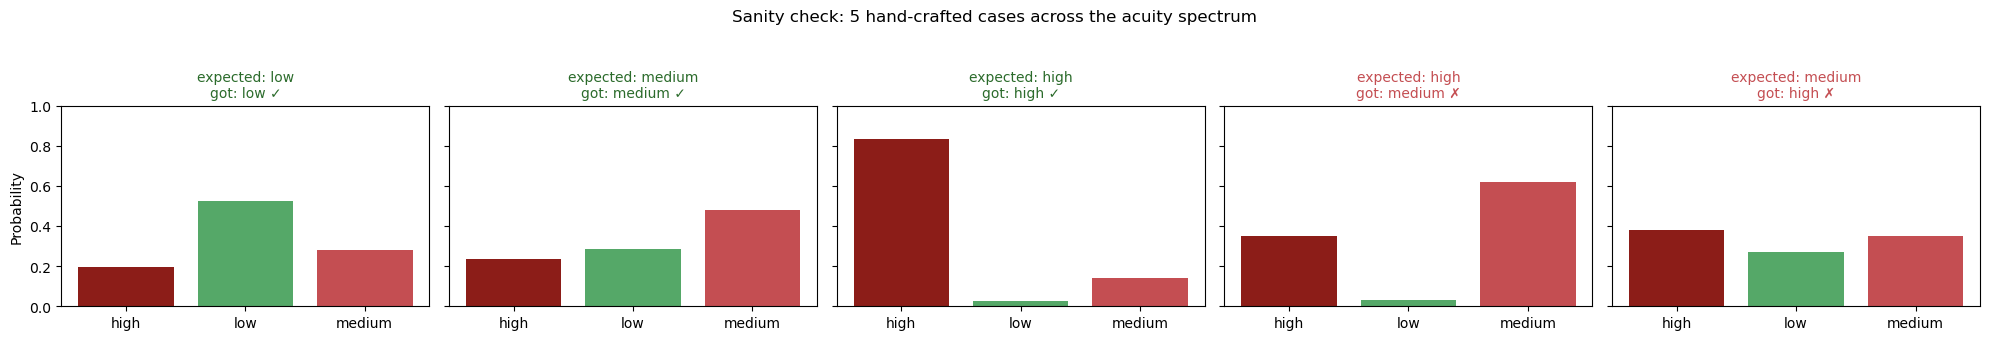
\includegraphics[width=\linewidth]{fig_triage_sanity.png}
  \caption{Predicted tier probabilities for the cases of Tab.~\ref{tab:triage-sanity}. The
    septic-shock-like presentation, where several vital signs are simultaneously abnormal, is
    the only one graded with high confidence (0.832); the remaining four distribute their mass
    across two or three tiers. This is a behavioural check on constructed inputs, not a
    performance measure.}
  \label{fig:triage-sanity}
\end{figure}

Both failures are confusions between \emph{adjacent} tiers, and neither confuses low with high
in either direction. They are not equivalent, however. The febrile young adult is over-triaged
at 37.9\% confidence --- the harmless direction, and without conviction. The elderly patient
with severe chest pain is under-triaged at 61.9\%, which is the combination that matters: the
wrong direction, stated with some confidence.

That case is the reason the tier is never the sole determinant of urgency. Reaching the
reasoning layer as \emph{medium}, it can still be escalated by an imaging finding, a missing key
laboratory value, or disagreement between the agents.

\subsubsection{Calibration}

Confidence is calibrated by Platt scaling fitted on a held-out slice of the training data,
never on the test set. Expected calibration error falls from 0.044 to 0.036.

That is a real improvement and a small one, because the model was already reasonably
calibrated. It is worth stating plainly what calibration did and did not do: accuracy is
essentially unchanged. Calibration does not make a model more accurate; it makes its stated
confidence mean something, which is what allows the reasoning layer to weigh a triage tier
against an imaging finding on a comparable scale.

\subsubsection{Final Decision}

The retained configuration is a gradient-boosted tree ensemble over the three-tier target,
trained on a temporal split with moderate class weighting, Platt-calibrated, and guarded by a
safety threshold of 0.20 on the high-urgency probability.

The limitations declared to the reasoning layer are that the model sees no imaging, that its
accuracy varies by source from 0.617 to 0.789, and that it estimates urgency rather than
diagnosis.

\subsubsection{Two Models, and Why There Are Two}
\label{subsec:triage-deployment}

The model described above is fitted on the full manifest, and part of its signal comes from
fields a hospital registration system assigns: the coded reason-for-visit categories, and the
source and year of the record. A clinician entering a patient at the bedside supplies none of
those. The intake screen asks for a presenting complaint in free text.

Restricting the fitted model to what the intake does supply was measured rather than assumed,
and the result was decisive: accuracy fell from 0.680 to 0.495, and on the held-out split the
model stopped predicting \textsc{low} altogether. A model starved of the features it was fitted
with is not the model whose accuracy was reported, and deploying it that way would put a figure
in this report that no deployed prediction could reach.

\begin{keystatement}
The response was not to restrict the model but to fit a second one, on exactly the fields the
interface collects. Training features, interface fields and deployment inputs are the same set.
\end{keystatement}

That second model is trained by the same procedure as the first --- the same temporal split, the
same class weighting, the same calibration slice carved out of the training data, the same
safety threshold --- so the two differ in their features and in nothing else.

\begin{table}[H]
  \centering
  \small
  \begin{tabular}{lrr}
    \toprule
    & \textbf{Reference} & \textbf{Deployed} \\
    \midrule
    Macro F1                    & 0.666 & 0.567 \\
    Accuracy                    & 0.680 & 0.630 \\
    Expected calibration error  & 0.036 & \textbf{0.030} \\
    Recall, \textsc{high}       & 0.784 & 0.773 \\
    Recall, \textsc{medium}     & 0.595 & \textbf{0.700} \\
    Recall, \textsc{low}        & \textbf{0.638} & 0.232 \\
    True \textsc{high} graded \textsc{low} & 1.55\% & \textbf{1.36\%} \\
    \bottomrule
  \end{tabular}
  \caption{The reference model and the deployed model on the same held-out split of 16,180
    visits. The deployed model is fitted on 21 features derived from the ten the intake
    collects; the reference model adds the registration fields.}
  \label{tab:triage-two-models}
\end{table}

The headline metric is lower, and the loss is not spread evenly. Recall on \textsc{high} is
essentially preserved and the dangerous miss --- a genuinely high-acuity patient graded
\textsc{low} --- is slightly \emph{better} than the reference model's. Almost the whole cost
falls on \textsc{low}: without the registration fields the model cannot confidently identify
low-acuity patients and errs towards \textsc{medium} instead. For decision support that is the
safe direction to lose accuracy in, and it is worth saying so explicitly rather than letting a
reader infer it from a table.

\paragraph{The two are registered separately.} Offering the deployed model as a replacement for
the reference model was tried and refused by the promotion gate of
Section~\ref{subsec:mlops}, for a macro-F1 regression of 0.099 that was both true and beside
the point. The gate compares successive versions of one model on one task; these are two models
answering different questions --- what the classifier achieves given complete records, and what
it achieves given what is actually typed. They now occupy separate production lines with
identical rules and unloosened tolerances, so a future deployed model is compared against the
deployed model it would replace and never against an artefact it was never built to beat.

\subsubsection{Suggestion, Confirmation, and Who Decides}

The deployed model does not set the urgency tier. It proposes one, and the clinician confirms
or changes it; the tier that reaches the reasoning layer is whichever the clinician left in the
control.

The interface shows the proposal and the observations it rests on, in clinical terms --- the
suggested tier, and either \emph{based on all recorded observations} or a count and the names
of those not taken. It does not show the probability vector, the model's name, or its
evaluation figures. A screen reporting \emph{0.646 medium, macro F1 0.567} asks a reader to
audit a classifier when their task is to see a patient, and those figures belong in this report
rather than at the bedside.

What is recorded with the encounter is fuller than what is displayed: the suggested tier, the
probability distribution behind it, the tier the clinician settled on, which observations were
available, and whether the two agreed. The record is written by the server from the state at
the moment of assessment, not accepted from the request, because a record a caller can write is
not a record --- it could report an agreement that never happened.

\begin{keystatement}
When the two differ, the system records that they differ. It does not record that the model was
wrong, because it has no ground truth with which to decide that.
\end{keystatement}

\paragraph{A defect this exposed.} The urgency control did not exist until late in the project.
The intake form carried a fixed value of \textsc{medium} and sent it with every encounter, so
the escalation trigger that fires when triage and imaging disagree could not fire for any
patient entered through the interface. The rule was correct throughout and its own tests passed,
because those tests call the conflict detector directly with a \textsc{low} tier. A rule can be
correct and never run, and no test that exercises the rule can reveal that: it took following
the value from the screen to the reasoning layer. The end-to-end checks added with the control
traverse that path over HTTP, which is where the gap was.

\paragraph{A second defect, in the suggestion itself.} The first implementation read the
model's probability vector in clinical order --- low, medium, high. The label encoder sorts its
classes, so the columns are ordered high, low, medium, and a hypotensive, hypoxic, tachycardic
81-year-old arriving by ambulance was graded \textsc{low} urgency at 0.87. Nothing raised: the
shapes matched, the probabilities summed to one, and every field was populated. The mapping is
now read from the artefact rather than written as a literal, and a test compares two
constructed patients by \emph{order} rather than by label, so that it survives retraining and
still fails if the vector is ever inverted again.

% =========================================================================================
\subsection{Ultrasound Agent: Organ Routing}
\label{subsec:ultrasound-agent}

The Ultrasound Agent presents one entry point. A study arrives with an organ and the
appropriate inputs --- two frames for cardiac, one still for gallbladder, a list of frames for
lung --- and is dispatched to the module that handles it.

An organ with no implemented module is not omitted and is not answered with a low-confidence
guess. It returns \texttt{status: "not\_supported"} in the ordinary output format, with an
empty finding list and a scope note. Vascular and FAST are in this position.

The consequence is that the reasoning layer never branches on whether a key exists. An
unsupported organ and an assessed one differ in the value of a field, not in the shape of the
object, and the distinction between ``examined and negative'' and ``never examined'' is carried
explicitly rather than inferred from an absence. Section~\ref{subsec:output-contract} describes
the contract this relies on.

\subsubsection{From notebook to importable module}
\label{subsubsec:agent-extraction}

The per-organ prediction code originally lived only in a Jupyter notebook. Nothing outside a
Colab session could execute it, and consequently no automated test could import it: the suite
proved that the output contract was \emph{enforced}, and could not prove that any perception
module \emph{honoured} it. That gap was reported as a limitation of this work.

It has since been closed for all three organs. The prediction code was extracted into an
importable module and is now exercised by sixteen tests grouped under a new safety property,
\emph{perception contract}, each running real inference on the shipped checkpoints. The lung
module was extracted first, and the cardiac and gallbladder modules followed once their
checkpoints and calibrators were retrieved from the training runs.

Two findings came out of the extraction, and both are more instructive than the extraction
itself.

\paragraph{The architecture had to be recovered from the checkpoints, not from the notebook.}
The two disagree. The notebook builds a two-layer classification head; every shipped checkpoint
contains a single linear layer of shape $4 \times 1280$. Loading the weights non-strictly
succeeds and leaves the mismatched layers at their random initialisation --- silently, and with
no error at any point. The architecture was therefore reconstructed from the checkpoint itself
and is now loaded strictly, so that any future divergence fails loudly instead of producing a
model that runs and means nothing.

\paragraph{The first test found a defect that had silenced the model.} The lung calibration
artefact described in Section~\ref{subsubsec:lung-calibration} was never exported from the
training notebook to a file. Both the notebook and the extracted module therefore fell back to
a decision threshold of $0.5$ for every finding. This model's outputs are compressed into
roughly the interval $[0.2, 0.8]$, so at $0.5$ almost nothing crosses: every study returned an
empty finding list, which the layers downstream read as a scan that was performed and showed
none of the modelled pathologies.

The failure is worth dwelling on because of its direction. A screening module that reports
false positives is annoying; one that silently reports every patient as clear is dangerous, and
it produces no error, no warning and no visible symptom. It was invisible precisely until the
code became importable and something asserted a property of it.

The tuned operating points had been written to disk by the training run all along, in the
per-split results files: $0.30$, $0.20$, $0.35$ and $0.45$ for B-lines, consolidation, pleural
effusion and pleural thickening respectively. The module now reads them back.

The correction was verified on LUS-BALD, an independent B-line localisation dataset that this
classifier never saw in training. Over 120 B-line-positive studies, the B-line output averages
$0.813$ and crosses its tuned threshold on every one of them, against an area under the ROC
curve of $0.919$ measured between those studies and random noise. Consolidation, correctly, sits
at $0.155$ on the same images --- and fires on none of them at a threshold of $0.5$. The model
was never the problem; the operating point was.

A distinction that the episode makes concrete, and that is easy to elide: a threshold states
\emph{where the decision boundary sits}, and calibration states \emph{what the number means}.
The thresholds were recovered. The Platt calibrators were not, and are genuinely lost, so the
deployed module continues to report \texttt{confidence\_calibrated: false} and emits a raw
sigmoid output. The boundary is tuned; the number is not.

\paragraph{Extracting the other two found three more defects, all of the same kind.} Cardiac and
gallbladder inference was extracted once their checkpoints were retrieved. The gallbladder
module transferred without incident. The cardiac module did not, and each of its three faults
produced a plausible output rather than an error --- which is why none had been noticed.

The first is a matter of arity. Ejection fraction is a \emph{comparison} between end-diastole
and end-systole, so a single still cannot produce one. Handed one frame as both, the arithmetic
computes a fractional change of zero and reports a normal ventricle. The interface now requires
both frames and refuses with a stated reason rather than returning a number.

The second is the serious one, and it was observed on real echocardiographic frames rather than
hypothesised. The systolic area was not checked for zero. A frame in which the segmentation
found no ventricle therefore entered the formula as an area of $0$, which the expression reads
as a ventricle that has ejected \emph{all} of its volume: an ejection fraction of 100\,\%,
banded \emph{normal}, and reported at the calibrator's maximum confidence. The direction of that
error is what makes it serious --- a failed measurement became a reassuring one. A frame in
which the ventricle cannot be found is a failed measurement, not a measurement of zero, and the
module now requires both areas to be non-zero, requires at least half the augmented views to
yield a usable pair, and treats a derived ejection fraction above 85\,\% as evidence of a
collapsed systolic segmentation rather than of a hyperdynamic heart.

The third is that calling the router without an image raised an exception. Every other
degradation in this system arrives as a report carrying \texttt{status: "failed"}, and this one
now does too, so the reasoning layer never has to catch an exception in order to stay correct.

\paragraph{An in-domain check, now that the module can be run outside a notebook.} The cardiac
module was evaluated against CAMUS's own recorded ejection fraction over thirty patients, using
the dataset's designated end-diastole and end-systole volumes. Twenty-eight produced a reading,
with a mean absolute error of 6.3 percentage points and a median of 5.2 --- consistent with the
6.9 reported from the training run in Section~\ref{subsec:cardiac-module}. The two refusals were
the patients with the highest true ejection fractions in the sample, where the module's upward
bias carries the estimate past the implausibility bound. That bound was left where it was rather
than adjusted after seeing which patients it caught, since tuning a threshold against the cases
it fails on is how a result becomes optimistic without anyone intending it.

The same run makes the generalisation gap of Section~\ref{subsec:cardiac-module} concrete. On an
echocardiographic source outside CAMUS the module segments a left ventricle averaging 157 pixels
against a myocardium of 954 --- an implausible ratio --- and the guards above refuse to produce a
band from it. The refusal is the correct behaviour and is also a measurement: the module does not
transfer, and it now declines rather than reporting a number from a segmentation it should not
trust.

% =========================================================================================
\subsection{Lung Module}
\label{subsec:lung-module}

\subsubsection{Objective}

The lung module detects four findings in a lung ultrasound clip: B-lines, consolidation,
pleural effusion and pleural thickening.

It is deliberately not a disease classifier. It reports what is visible in the images, and the
inference from B-lines to pulmonary oedema, or from consolidation to pneumonia, belongs to the
reasoning layer, which has access to the vitals, laboratory results and history that such an
inference requires. A module that reported ``pneumonia'' would be making a clinical judgement
from imaging alone.

\subsubsection{Dataset and the Multi-Label Formulation}

The four findings co-occur: a clip can show B-lines and a consolidation at the same time, and
frequently does. The task is therefore multi-label --- four independent probabilities --- rather
than single-label with one distribution over four mutually exclusive classes.

This is the first structural difference from the cardiac and gallbladder modules and it
propagates. It is the reason the shared schema carries a \emph{list} of findings rather than
one, and the reason the calibration section below fits four separate calibrators.

\subsubsection{Preprocessing and Clip Handling}

Eight evenly spaced frames are taken from each clip rather than every frame. Neighbouring frames
in an ultrasound clip are near-duplicates, so decoding all of them multiplies computation
without adding information. Frames are decoded once and cached.

Inference runs per frame and the frame probabilities are aggregated to a clip probability by
the \emph{median}. The choice matters and is not arbitrary. Frames from one clip are not
independent evidence about the patient; they are repeated looks at the same anatomy. The mean
would let one blurred or off-plane frame with an extreme probability drag the clip result, while
the median reports what the majority of the clip shows.

\subsubsection{Partially Labelled External Data}

Additional images were available that are labelled positive for B-lines only. They carry no
negatives and no labels at all for the other three findings. Treating the missing labels as
negatives would teach the model that these images show no consolidation, no effusion and no
thickening, none of which is known.

The solution is a per-sample mask applied to the loss, restricting each sample's gradient to
the columns whose labels are actually known. A B-lines-only image contributes to the B-lines
output and to nothing else.

The discipline around this matters as much as the mechanism: these samples entered the
\emph{training} set only. They never appear in validation, so no reported figure is computed
over data with partially invented labels.

\subsubsection{Model Selection and the Frozen-Backbone Discovery}

The single most valuable diagnostic in this project came from a configuration that was not
working. An earlier setup froze the entire EfficientNet-B0 backbone and trained only the
classifier head, on the standard reasoning that a small dataset cannot support fine-tuning a
full network.

That reasoning fails for ultrasound. Frozen ImageNet features encode edges, textures and object
parts learned from natural photographs, and ultrasound speckle resembles none of them. A frozen
backbone cannot adapt its representation, so the trainable head was being asked to separate
findings using features that did not describe them. Unfreezing the last blocks with a low
learning rate produced the largest single gain recorded anywhere in this project.

The general lesson is worth more than the specific gain: transfer learning assumes the source
and target domains share low-level structure, and that assumption should be checked rather than
inherited.

\subsubsection{Training}

Training used mixed precision, a cosine learning-rate schedule, and early stopping on validation
AUROC with a patience of three epochs against a budget of fifteen. Most folds stopped early. The
schedule is unremarkable and is reported for reproducibility rather than because anything was
learned from it.

\subsubsection{Results}
\label{subsec:lung-results}

Evaluation is 3-fold \texttt{GroupKFold} by case over 187 clips from 165 independent cases, with
predictions pooled out of fold and thresholds tuned on the folds not being evaluated.

\begin{table}[H]
  \centering
  \small
  \caption{Lung findings, pooled out-of-fold over 187 clips from 165 cases. ``pos'' is the
    number of positive clips available for that finding.}
  \label{tab:lung-results}
  \begin{tabular}{@{}lccccc@{}}
    \toprule
    Finding & AUROC & AP & Sensitivity & ECE & pos \\
    \midrule
    B-lines & 0.830 & 0.695 & 0.841 & 0.169 & 63 \\
    Consolidation & 0.832 & 0.726 & 0.600 & 0.146 & 60 \\
    Pleural effusion & 0.718 & 0.212 & 0.750 & 0.158 & 24 \\
    Pleural thickening & 0.773 & 0.453 & 0.652 & 0.195 & 46 \\
    \midrule
    \textbf{Macro} & \textbf{0.788} & & & & \\
    \bottomrule
  \end{tabular}
\end{table}

An earlier version of this evaluation reported AUROC between 0.745 and 0.808 and looked
comparable. It was inflated twice over: it split by clip rather than by case, so clips from the
same patient appeared on both sides of the split, and it tuned decision thresholds on the same
data it evaluated them on. Both inflations were removed and the figures above are the
defensible ones. They are reported here rather than the more flattering earlier numbers, and
the earlier numbers are reported alongside so that the difference is visible.

Pleural effusion is marked unreliable. Its 24 positive clips are too few to support a stable
threshold, and its average precision of 0.212 --- against an AUROC of 0.718 --- shows the
instability directly: the ranking is better than chance while the operating point is poor. That
mark is carried through the output contract to the reasoning layer, which discounts the finding
rather than weighing it like the others.

Pneumothorax is not modelled at all. The dataset contains zero positive cases, so no threshold
could be set and no confidence would mean anything. This absence is declared as a scope
limitation, and it is why an all-negative lung scan escalates in
Section~\ref{subsec:reasoning-escalation} rather than reading as reassurance.

\subsubsection{Error Analysis}

The two findings the model handles best, B-lines and consolidation, are also the two with the
most positive cases (63 and 60). The two it handles worst, pleural thickening and pleural
effusion, have 46 and 24. The ordering of performance follows the ordering of positive-case
counts exactly, which is the most parsimonious explanation available and does not require
appeal to intrinsic difficulty.

The clinically relevant confusions are between findings that co-occur: effusion and
consolidation appear together in the same clinical presentations, and a clip showing both gives
the model correlated evidence for each. Because the formulation is multi-label the model is not
forced to choose between them, which is the correct behaviour, but it also means the four
outputs are not independent and per-finding figures should not be multiplied together as if
they were.

\subsubsection{Calibration}
\label{subsubsec:lung-calibration}

Each finding receives its own Platt-scaled calibrator, fitted out of fold. One calibrator for
all four would be wrong: the four heads are miscalibrated to different degrees, as the ECE
column of Table~\ref{tab:lung-results} shows, ranging from 0.146 to 0.195.

Decision thresholds are tuned on the folds not being evaluated and applied to the held-out one.
Tuning and evaluating a threshold on the same data reports the best case rather than the
expected case, and was one of the two inflations removed from the earlier evaluation.

One limitation of the calibration is stated rather than hidden: it is fitted and scored on the
same out-of-fold predictions, so the reported ECE is optimistic.

A second limitation is procedural rather than statistical, and cost more. The calibrators were
fitted inside the training notebook and never written to a file, so nothing downstream could
load them. The consequences of that omission, and the recovery of the tuned thresholds from the
per-split results files, are described in Section~\ref{subsubsec:agent-extraction}. The
thresholds were retrievable; the calibrators were not. An artefact that exists only in the
memory of a notebook session does not exist.

\paragraph{Whether they could simply be refitted.} The obvious remedy is to regenerate the
out-of-fold predictions and fit the calibrators again. That was examined and rejected, on the
data rather than on effort. Calibration must be fitted on cases held out from both training
and threshold tuning, or the resulting probabilities are fitted to the same evidence they are
later scored against. Carving such a split out of this dataset leaves too little to fit
anything on:

\begin{table}[H]
  \centering
  \small
  \begin{tabular}{lrrr}
    \toprule
    \textbf{Finding} & \textbf{Positive clips} & \textbf{Positive cases} &
    \textbf{In a 20\% split} \\
    \midrule
    B-lines             & 63 & 53 & $\approx$ 11 \\
    Consolidation       & 60 & 46 & $\approx$ 9 \\
    Pleural thickening  & 46 & 39 & $\approx$ 8 \\
    \textbf{Pleural effusion} & \textbf{24} & \textbf{16} & $\approx$ \textbf{3} \\
    \bottomrule
  \end{tabular}
  \caption{Case-level positives per lung finding, and what a held-out calibration split would
    contain. The unit is the case, not the clip, for the reason established in
    Chapter~\ref{sec:data}.}
  \label{tab:lung-calibration-budget}
\end{table}

A Platt scaling fitted on three positive cases is not a calibration; it is a curve through
noise that would then be printed beside a clinical finding as a probability. The decision was
therefore to leave the module uncalibrated and to say so everywhere the number appears: the
report declares \texttt{confidence\_calibrated: false}, the scope string states that the
confidence is a raw sigmoid output and that the decision boundary is tuned while the number is
not, and \texttt{/api/health} reports the module as \emph{ready, uncalibrated}.

\begin{keystatement}
Reporting a raw score labelled as raw is honest. Manufacturing a calibration from three
positive cases and labelling it calibrated is not, and the label is what a clinician would
act on.
\end{keystatement}

This is the one place where the lung module is deliberately weaker than the cardiac and
gallbladder modules, which do carry fitted calibrators. It is a consequence of the dataset
size, not of the method, and it is the first thing additional lung data would fix.

\subsubsection{Final Decision}

The retained configuration is EfficientNet-B0 with the last blocks unfrozen, multi-label over
four findings, median aggregation across eight frames per clip, per-finding Platt calibration
and per-finding thresholds tuned out of fold.

The declared limitations are that pneumothorax is not modelled and cannot be excluded, that
pleural effusion is unreliable, that the module has no healthy class so an empty finding list
never means a normal study, and that the data are curated public clips rather than bedside
acquisitions.

% =========================================================================================
\subsection{Cardiac Module}
\label{subsec:cardiac-module}

\subsubsection{Objective}

The cardiac module segments the left ventricle, myocardium and left atrium in an
echocardiographic view, and derives an ejection fraction from the segmentation at end-diastole
and end-systole. The finding it reports is an EF band --- normal, reduced or severe --- with a
calibrated confidence.

It is the only pixel-level model in the system. Every other module classifies; this one labels
each pixel and computes a clinical quantity from the result, which makes its error analysis
different in kind from the others.

\subsubsection{Dataset}

Training uses CAMUS, which provides explicit patient structure and expert annotations, split by
patient. An additional external collection is used for validation only and never for training.
Provenance is in Chapter~\ref{sec:data}.

In-domain results are read against the published nnU-Net figures on CAMUS discussed in
Section~\ref{subsec:sota-existing}: Dice of 0.93 for the left ventricle, 0.86 for the myocardium
and 0.89 for the left atrium.

\subsubsection{Model and Loss}

The architecture is a U-Net with an EfficientNet-B0 encoder, 6.25 million parameters.

The loss combines cross-entropy with soft Dice, and the combination is necessary rather than
conventional. The structures of interest occupy a small fraction of the image, so a model
minimising cross-entropy alone can achieve a low loss by predicting background almost
everywhere: the pixel-wise objective is dominated by the majority class. Soft Dice measures
overlap between the predicted and true regions directly, and is insensitive to the size of the
background, so it rewards exactly what cross-entropy neglects.

Partially labelled masks are handled with an ignore index, so pixels whose true class is
unknown contribute no gradient rather than being treated as background.

\subsubsection{Training}

Early stopping monitors validation Dice, and the \emph{best} checkpoint is retained rather than
the last. The distinction matters when validation performance is non-monotone: keeping the last
checkpoint would report a model that had already begun to overfit.

\subsubsection{In-Domain Results}
\label{subsec:cardiac-results}

On held-out CAMUS patients the module reaches Dice of 0.928 for the left ventricle, 0.837 for
the myocardium and 0.875 for the left atrium, against the benchmark figures of 0.93, 0.86 and
0.89.

The left ventricle is essentially at benchmark. The myocardium and left atrium sit slightly
below. The left atrium is the weakest structure here, as it is in the published results ---
it has less consistent boundary contrast than the ventricle and its extent depends on the
imaging plane --- and reporting it as the weakest rather than averaging the three into one
number is what makes the comparison meaningful.

\subsubsection{External Validation and the Generalisation Gap}

On the external collection, left-ventricle Dice falls from 0.928 to 0.534. The drop is large
and is reported with both numbers rather than as a percentage.

The investigation proceeded in three steps, and the order is worth preserving because the
second step overturned the first.

\begin{enumerate}
  \item \textbf{A hypothesis formed from a handful of images.} Inspecting a small number of
        external cases suggested a labelling-convention mismatch: the external masks appeared
        to include or exclude structures at the boundary differently from CAMUS, which would
        depress Dice without the model having failed to find the ventricle.
  \item \textbf{Connected-component analysis over the full dataset, which disproved it.}
        Measuring mask fragmentation across every external case gave 2.4\% --- the predictions
        are coherent single regions, not scattered fragments, and the geometry does not show
        the systematic boundary offset the hypothesis predicted. The hypothesis was formed from
        a sample too small to support it and was abandoned.
  \item \textbf{What remains.} The gap is a genuine domain shift: different acquisition
        equipment, different operators, different imaging conventions. What it is \emph{not} is
        a labelling artefact, and it is not the model failing to localise the ventricle at all.
\end{enumerate}

The reversal is reported as method rather than concealed as an embarrassment. A conclusion
drawn from a handful of images and overturned by measurement over the full dataset is the same
error, in miniature, that the gallbladder module also produced
(Section~\ref{subsec:gallbladder-module}), and the recurrence is why it is stated twice.

Fig.~\ref{fig:cardiac-external-grid} shows what that failure looks like on individual frames,
and the visual form matters as much as the number. The predicted regions are single, smooth and
correctly placed over the ventricle; they are simply too small, cut off well inside the true
boundary. That is the signature of a decision threshold displaced by domain shift, not of a
model searching in the wrong part of the image.

\begin{figure}[H]
  \centering
  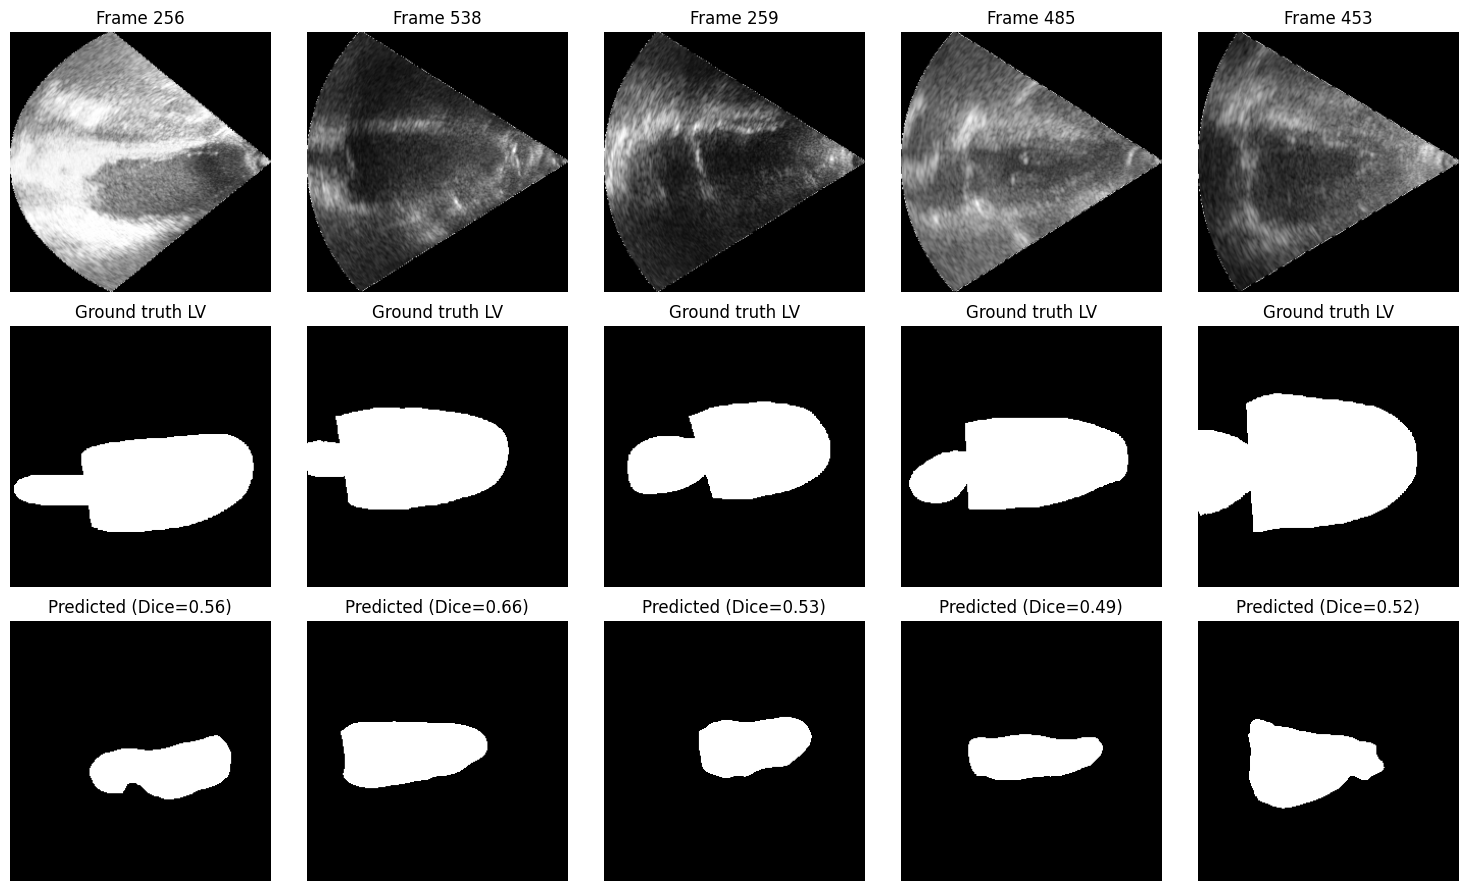
\includegraphics[width=\linewidth]{fig_cardiac_external_grid.png}
  \caption{Five frames drawn at random from the external collection: the image, the reference
    left-ventricle mask, and the prediction with its own Dice. The five values, 0.49 to 0.66,
    bracket the collection mean of 0.534 and are therefore representative rather than selected.
    Every prediction is one coherent region in approximately the right place and every one
    under-segments, which is the same conclusion the fragmentation measurement reached and the
    opposite of what a localisation failure would look like.}
  \label{fig:cardiac-external-grid}
\end{figure}

\subsubsection{Ejection Fraction}

Ejection fraction derived directly from segmented \emph{areas} carried a systematic bias: mean
absolute error of 12.2 percentage points against the reference values, with a correlation of
0.788.

The explanation is geometric rather than statistical. Ejection fraction is defined over
volumes, and area does not scale with volume: for a roughly ellipsoidal chamber, volume grows
as area to the power of $3/2$. Computing a fractional change from areas therefore understates
the fractional change in volume, systematically and predictably.

Applying the correction $\mathrm{EF} = \bigl(1 - r^{3/2}\bigr) \times 100$, where $r$ is the
ratio of end-systolic to end-diastolic area, reduced the mean absolute error from 12.2 to 6.9
percentage points --- a bias of 5.3 points removed --- and raised the correlation slightly to
0.795.

The result here is not the improved number. It is the agreement between the bias predicted from
the geometry and the bias actually observed. A correction derived from theory and then confirmed
by measurement is worth considerably more than a constant tuned until the error dropped, because
it will continue to hold on data this project has not seen.

On the three-band classification the module reaches a balanced accuracy of 63.4\% against a
chance level of 33.3\%. Plain accuracy is 65.0\% against a majority baseline of 66.0\%, and the
comparison shows why plain accuracy is the wrong headline: 66 of 100 patients fall in one band,
so predicting that band for everyone scores higher than the model while discriminating nothing.

Per-band recall is 0.727 for severe ($n=11$), 0.697 for reduced ($n=66$) and 0.478 for normal
($n=23$). The clinically important figure is the last line of the confusion matrix: \textbf{zero
of 100 cases confused a severe ventricle with a normal one}. The dangerous error --- reading a
failing heart as healthy --- did not occur in this cohort, though with 11 severe cases that is
a bound rather than a guarantee.

\subsubsection{A Small Error at a Cutoff is a Category Error}
\label{subsec:cardiac-boundary}

A mean absolute error of 6.9 points reads as a good result, and on its own it is. But the number
is not what a clinician acts on --- the band is, and the bands are separated by cutoffs at 30
and 55. An error far smaller than the reported average can move a patient across one.

The effect is visible on individual cases. Estimating a reference ejection fraction of 29 as 31
is a numeric error of 2.0 points, well inside the module's typical accuracy, and it changes the
clinical statement from \emph{severe} to \emph{moderate} dysfunction. The same arithmetic
applies at the upper cutoff, where an error of 3.7 points moved a reference value of 54 to 57.7
and turned a mildly reduced ventricle into a normal one.

The module therefore reports, with every ejection fraction, how far that value sits from the
nearest cutoff and whether it lies within the module's own measured error of one.

\begin{keystatement}
The margin is the module's held-out mean absolute error, not a chosen number. It is an
engineering sensitivity zone: it says this model cannot resolve which side of the cutoff the
patient is on, not that a cardiologist would call the value borderline.
\end{keystatement}

The distinction matters because a margin invented for the purpose --- five points, three points
--- would be presented to a clinician as though it carried clinical meaning. Deriving it from
the measured error makes it a statement about the instrument, which is what it is.

The consequence is visible and worth stating plainly: because 6.9 points is wide relative to a
\emph{reduced} band only 25 points across, a substantial share of predictions fall inside the
zone and are flagged. That is the honest reading of an error of this size, and a narrower margin
chosen to reduce the flag rate would have missed both of the band crossings described above.
This is also the reason balanced accuracy over the three bands, at 63.4\%, is a far less
flattering headline than the 6.9-point error --- and the more truthful one.

\subsubsection{Rejected Adaptations}

Six strategies were tried against the external gap and four were rejected.

\begin{table}[H]
  \centering
  \small
  \caption{Adaptations tested against the cardiac generalisation gap.}
  \label{tab:cardiac-rejected}
  \begin{tabularx}{\textwidth}{@{}lXl@{}}
    \toprule
    Strategy & Hypothesis and outcome & Decision \\
    \midrule
    Augmentation upgrade & Stronger augmentation would cover the domain shift; the measured
      difference was within run-to-run variation & rejected \\
    External integration (2 ways) & Adding external data to training would bridge the gap; both
      integrations degraded in-domain performance without closing it & rejected \\
    Fine-tuning (2 ways) & Fine-tuning on the external set would adapt the representation; it
      improved the external number substantially while degrading CAMUS performance to an
      unacceptable degree & rejected \\
    Volume correction & Area-derived EF is biased by a predictable geometric factor; MAE
      12.2\,pp $\rightarrow$ 6.9\,pp & \textbf{retained} \\
    \bottomrule
  \end{tabularx}
\end{table}

Fine-tuning is the instructive rejection. It worked, in the narrow sense that the external
number improved substantially. It was rejected because the improvement was purchased with
in-domain performance, and the in-domain distribution is the one the module is declared to
serve. A model that performs moderately everywhere and well nowhere is not obviously preferable
to one that performs well within a stated domain and declares that domain honestly.

The non-fine-tuned model was retained and its domain limitation is declared to the reasoning
layer rather than hidden by an averaged figure.

\subsubsection{Calibration}

Confidence is the fraction of eight fixed test-time augmentations that agree on the reported
band --- fixed rather than random, so the same clip always yields the same number --- and that
agreement fraction is calibrated by isotonic regression.

Isotonic regression suits this case because an agreement fraction is not a softmax output and
its distortion is not of a form a single temperature parameter can correct; a non-parametric
monotone fit can. Expected calibration error falls from 0.314 to 0.060, by far the largest
calibration correction of any module, which reflects how poorly a raw agreement fraction
behaves as a probability.

The isotonic fit also implies a confidence ceiling: the calibrator maps even unanimous
agreement to a value below 1.0, and that ceiling is declared in the output so that no
downstream component treats the module as certain.

\subsubsection{Final Decision}

The retained model is the CAMUS-trained EfficientNet-B0 U-Net without fine-tuning, with
volume-corrected ejection fraction reported as a three-band finding and isotonic-calibrated
confidence.

The declared scope is explicit: CAMUS-like four-chamber views, ejection fraction as an area
proxy rather than a volumetric measurement, and a documented drop on out-of-domain
acquisitions. What this forbids the reasoning layer from concluding is that the module's
confidence is meaningful on an image unlike its training domain --- and because the module
cannot tell whether a given image is in domain, that judgement is left to the clinician, with
the limitation stated in every report.

% =========================================================================================
\subsection{Gallbladder Module}
\label{subsec:gallbladder-module}

\subsubsection{Objective}

Single-label classification of gallbladder pathology at case level, over five reported classes:
cholelithiasis, acute cholecystitis, polyps and adenomyomatosis, carcinoma, and wall thickening.

\subsubsection{Dataset and the Mislabelled Class}

The dataset comprises 4\,826 frames from 199 cases, organised as nine folders by pathology.

A per-case inspection found that one folder's contents did not match its label. The
methodological history of that finding is more valuable than the finding itself. The class had
first been judged from a handful of frames drawn from a small number of cases, and looked
consistent. Sampling one frame per case across all cases in the folder reversed the conclusion
immediately.

The rule this establishes generalises well beyond this dataset: \textbf{frames from one case are
not a sample of a class}. A handful of frames from two cases shows what those two cases look
like, and any impression formed from them describes the cases rather than the category. The same
error appeared independently in the cardiac module, where a hypothesis formed from a few images
was overturned by measurement over the full dataset.

The affected folder was excluded, reducing the taxonomy from nine classes to eight for training.

\subsubsection{Taxonomy Selection}

Several groupings of the eight training classes into a reported taxonomy were plausible. Training
a model per candidate would have cost GPU time proportional to the number of candidates.

Instead, the confusion matrix already measured from the fine-grained model was collapsed
arithmetically according to each candidate grouping, estimating the accuracy each would achieve
without training anything. The candidate that this predicted would perform best was the one
taken forward, and it predicted 63.0\% balanced accuracy for collapsing the fine-grained model's
predictions.

The measured result after training the chosen configuration was 59.7\%. The agreement between a
prediction made from an existing confusion matrix and a figure measured after training is itself
a result: it justifies having spent GPU time on one configuration rather than several, and the
three-point shortfall marks the limit of the approximation rather than invalidating it.

\subsubsection{Training}

The model trains on the eight fine-grained labels and reports five, with class weights computed
per fold from the training portion only --- computing them over the whole dataset would leak the
test distribution into training.

The marginalisation from eight classes to five sums group probabilities rather than mapping the
argmax. The distinction is not cosmetic. A case whose probability mass is split across
cholecystitis, gangrenous cholecystitis and perforation --- three members of one reported group
--- has a high total probability of acute inflammation and no single dominant fine-grained class.
Mapping the argmax reports whichever member happens to be largest, discarding the agreement
between them; summing reports what the model actually believes about the group. Measured
directly, summing scored 63.0\% against 57.2\% for training on the merged labels.

\subsubsection{Results}
\label{subsec:gallbladder-results}

Evaluation is 5-fold \texttt{GroupKFold} by case, case-level predictions, over 199 cases with
frames capped at 25 per case so that longer studies do not dominate.

Balanced accuracy on the five reported classes is 59.7\% against a chance level of 20.0\%; plain
accuracy is 61.3\%. Per-class recall is given in Table~\ref{tab:gb-results}.

\begin{table}[H]
  \centering
  \small
  \caption{Gallbladder per-class recall, case level, with the one-standard-error bound at each
    class's case count.}
  \label{tab:gb-results}
  \begin{tabular}{@{}lcc@{}}
    \toprule
    Class & Cases & Recall \\
    \midrule
    Acute cholecystitis (any severity) & 66 & 0.70 $\pm$ 0.06 \\
    Carcinoma & 27 & 0.67 $\pm$ 0.10 \\
    Polyps / adenomyomatosis & 49 & 0.59 $\pm$ 0.07 \\
    Wall thickening & 25 & 0.56 $\pm$ 0.10 \\
    Cholelithiasis & 32 & 0.47 $\pm$ 0.09 \\
    \bottomrule
  \end{tabular}
\end{table}

The progression that produced this figure is worth reporting in full, because the improvement is
only interpretable against its starting point:

\begin{table}[H]
  \centering
  \small
  \caption{Balanced accuracy on the same 199 cases and the same reporting taxonomy.}
  \label{tab:gb-progression}
  \begin{tabular}{@{}lc@{}}
    \toprule
    Configuration & Balanced accuracy \\
    \midrule
    Original 9-class taxonomy, mislabelled folder included & 37.5\% \\
    Trained directly on the 5 merged classes & 57.2\% \\
    Collapsing the 9-class model's predictions & 63.0\% \\
    Retained: 8-class training, summed output, class-weighted & 59.7\% \\
    \bottomrule
  \end{tabular}
\end{table}

Grouping the five reported classes further into three clinical categories gives 63.6\% balanced
accuracy against a majority baseline of 50.8\%. That grouping is supported by the imaging only
weakly: 18\% of the fine-grained model's confusions stay inside their group, meaning most errors
cross group boundaries and the categories are not capturing a distinction the model can see.
The five-class output was retained on that basis.

\subsubsection{Rejected Alternatives}

Two alternatives were tested and rejected, both with the numbers that decided them.

\textbf{Training directly on merged labels} scored 57.2\% balanced accuracy against 63.0\% for
training fine-grained and merging probabilities afterwards. Collapsing the labels before
training discards the distinction between group members, and with it the model's ability to
accumulate evidence across them.

\textbf{USCL initialisation} was tested on the strength of the published gain discussed in
Section~\ref{subsec:sota-existing}: ultrasound-specific self-supervised pretraining should
transfer better to ultrasound than ImageNet weights. On a fold-0 bake-off it reached 29.8\%
balanced accuracy against 46.6\% for the ImageNet-initialised EfficientNet-B0 --- not a marginal
difference. The published result was not reproduced here, and the ImageNet initialisation was
retained.

\subsubsection{Calibration}

Temperature scaling, with a fitted temperature of $T = 0.87$. Expected calibration error moves
from 0.025 to 0.024.

The temperature below 1.0 indicates the model was mildly \emph{under}-confident rather than
over-confident, which is unusual and worth noting: the class-weighted loss, which penalises
errors on rare classes more heavily, appears to have flattened the output distribution slightly.
The correction is small because there was little to correct.

\subsubsection{Final Decision}

The retained configuration is EfficientNet-B0 trained on eight fine-grained classes with
per-fold class weights, reporting five classes by summing group probabilities, temperature
calibrated at $T = 0.87$.

The declared limitation that matters most is the absence of a healthy class. The dataset
contains no normal gallbladders, so every prediction is a choice among pathologies and none of
them means ``no disease''. The module therefore cannot exclude anything, and the reasoning layer
is told so explicitly: a gallbladder report is evidence about \emph{which} pathology, never
evidence that there is none. The remaining declared limitations are the 199-case sample, the
burned-in annotation markers present in 15--50\% of frames, and the teaching-atlas provenance.

\subsubsection{Reporting the Classes That Were Not Chosen}
\label{subsec:gallbladder-alternatives}

A module that names one diagnosis and stops leaves a reader unable to distinguish two very
different situations: a diagnosis that was weighed against the alternatives and preferred, and
a diagnosis reported because the alternatives were never in the label set at all. The lung
module does not have this problem --- it reports all four findings it screens, positive or
negative --- but a single-label module does, and the gallbladder module is single-label.

It therefore reports the four classes it ranked below the one it chose, with their
probabilities and the margin between the first and the second. On a cholecystitis case the
report reads: acute cholecystitis at 0.541, then cholelithiasis 0.234, carcinoma 0.175, polyps
0.039 and wall thickening 0.011.

\begin{keystatement}
These are not negative results. The five probabilities sum to one and describe one mutually
exclusive choice, so a class ranked lower was never screened for and found absent --- it was
outranked.
\end{keystatement}

The distinction is enforced in the schema rather than left to a convention. The ranked classes
occupy their own field, separate from the list of findings a module screened and did not see,
and a report carrying both is rejected as invalid: a module either screens independent findings
or chooses among exclusive ones, and one claiming to do both cannot be interpreted --- a reader
could not tell whether a label absent from the findings had been ruled out or merely outranked.

\paragraph{They are shown to the clinician and withheld from the language model.} The ranked
alternatives reach the interface but never enter the clinical state, and that is the point of
keeping them in a separate field. Everything in the clinical state becomes enumerated evidence
that the reasoning layer may cite; an alternative is not an observation about the patient but a
diagnosis the module considered and did not make. Citing ``cholelithiasis 0.23'' as evidence
would be fabrication with a number attached, and the separation makes it unrepresentable rather
than merely discouraged.

The margin is reported for a related reason. A confidence of 0.541 says how sure the module is;
it does not say how close the runner-up was. A margin near zero means the module effectively
could not separate two diagnoses, which is a different warning from low confidence and is not
recoverable from the top-line number alone.

% =========================================================================================
\subsection{Explainability Across the Imaging Modules}
\label{subsec:explainability}

Grad-CAM applies to all three imaging modules and is therefore treated once here rather than
three times.

The methodological point is that the maps were \emph{measured} rather than inspected by eye.
Looking at a dozen heatmaps and finding them plausible is not evidence; it is an invitation to
confirmation bias, since a viewer who knows where the pathology is will see the map pointing at
it. Three statistics were computed over the full sets instead:

\begin{itemize}
  \item \textbf{centroid spread} --- how much the centre of attention moves between images. A
        map that always points at the same place is responding to position rather than content;
  \item \textbf{area above half-maximum} --- what fraction of the image carries at least half
        the peak activation, which separates concentrated attention from diffuse;
  \item \textbf{normalised entropy} --- the dispersion of the attention distribution, referenced
        against the values for uniform attention (entropy 1.0) and for a single concentrated
        region.
\end{itemize}

An explicit test for centre bias accompanies them, because a heatmap that points at the middle
of every image regardless of content is not an explanation --- and ultrasound images place the
region of interest near the centre often enough that centre bias would look like success.

What these statistics support is that attention is concentrated and content-dependent rather
than uniform or positional. What they cannot support is that the attention falls on the
anatomically correct structure, which would require expert annotation of the relevant structure
in each image, and this project has none. The gallbladder module in particular showed a
pronounced central prior consistent with either a genuine anatomical focus or an acquisition
convention, and nothing measured here separates the two.

Fig.~\ref{fig:lung-gradcam} shows the lung maps, one clip drawn at random from the positives of
each of the four findings. It is included to make the measured statistics legible, and it
requires one caveat that the panel labels do not carry themselves.

\begin{figure}[H]
  \centering
  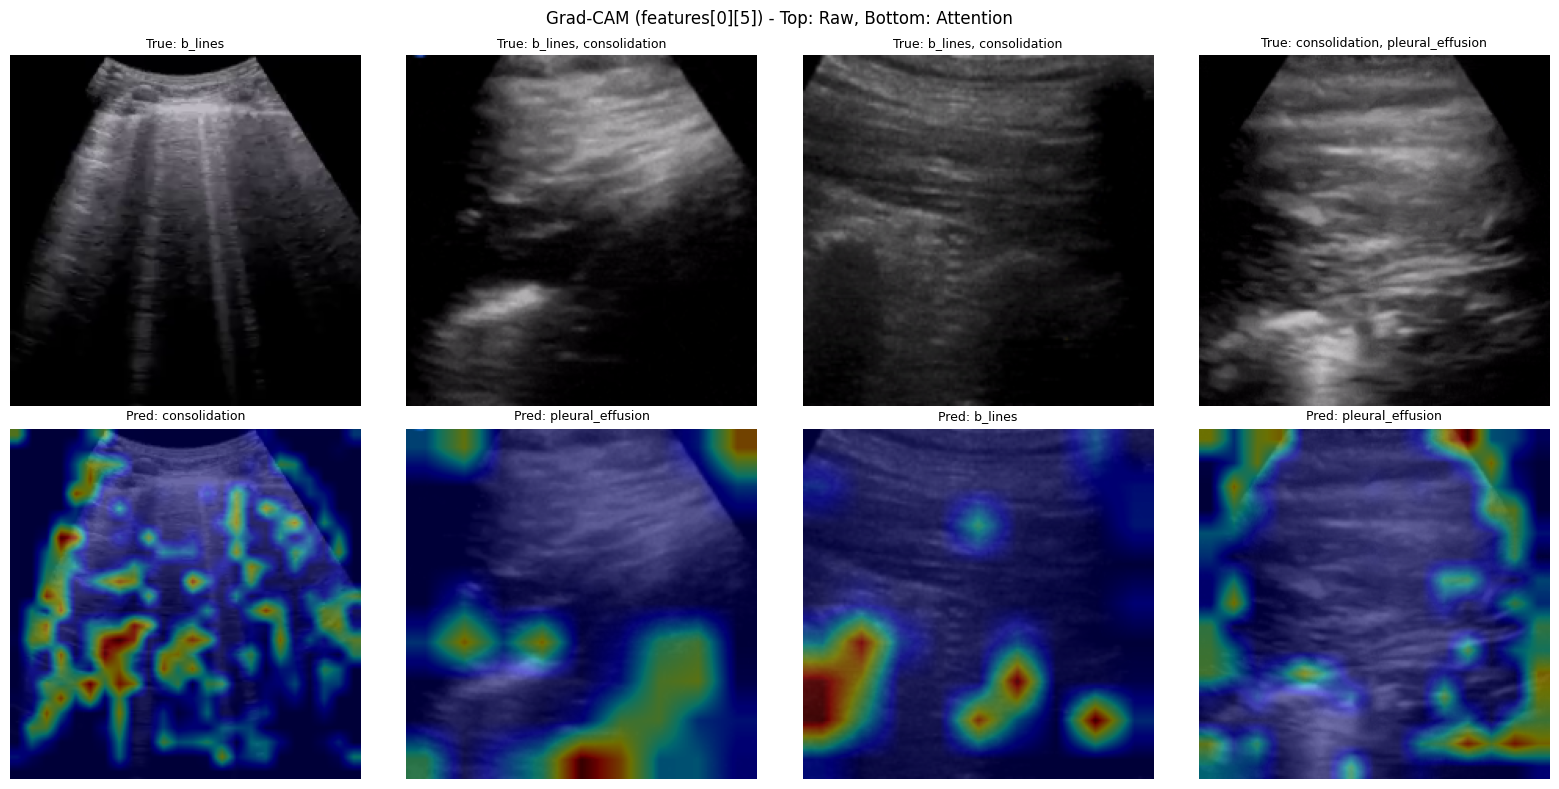
\includegraphics[width=\linewidth]{fig_lung_gradcam.png}
  \caption{Grad-CAM for the lung module: one clip per finding, top row the frame and bottom row
    the attention. The \textsc{pred} label is the \emph{highest-scoring} of the four findings,
    not the module's decision --- the module is multi-label and reports each finding
    independently against its own threshold, so a clip may carry two findings while only one
    can be named here. These panels therefore say nothing about whether the module classified
    the clip correctly.}
  \label{fig:lung-gradcam}
\end{figure}

The maps vary in how concentrated they are, and the first panel is the least concentrated of
the four. That is consistent with the statistics rather than in tension with them: the claim
established is that attention is concentrated \emph{on average} and moves with content, not
that every individual map is tight. Attention reaching the edge of the sector in several panels
is the observation that most warrants caution here, since the sector boundary is an artefact of
the acquisition geometry and carries no clinical information --- a model attending to it would
be reading the machine rather than the patient. Nothing measured here settles that, which is
why the boundary below is stated as firmly as it is.

Grad-CAM is therefore reported as a plausibility check that the models are not obviously
responding to the wrong thing, and explicitly not as evidence of clinical validity.
Section~\ref{subsec:results-explainability} states the same boundary at system level.

% =========================================================================================
\subsection{Perception Agent Output Contract}
\label{subsec:output-contract}

Every module writes through one schema. This section is the hinge between
Chapters~\ref{sec:perception} and~\ref{sec:reasoning}: it is what makes a segmentation network,
two classifiers and a tree ensemble usable by a single reasoning layer without that layer
knowing which produced what.

A report carries the organ, a status, a list of detected findings each with a calibrated
confidence, a list of findings screened for and \emph{not} detected, and a reliability block
declaring the module's scope.

Four validation rules are enforced, each for a reason established by a failure:

\begin{itemize}
  \item \textbf{Findings are always a list.} Lung is multi-label and a single-finding field
        could not represent a clip showing B-lines and consolidation together. Making the list
        universal means the reasoning layer never special-cases by organ.

  \item \textbf{A status of ``ok'' with nothing recorded is rejected.} A report claiming an
        assessment took place while recording neither a detected nor a screened-negative finding
        asserts nothing and would be indistinguishable downstream from an organ never examined.

  \item \textbf{A confidence above the declared ceiling is rejected.} The cardiac calibrator maps
        even unanimous test-time agreement to a value below 1.0; a report exceeding that ceiling
        indicates the calibration was not applied.

  \item \textbf{A label cannot appear in both the detected and not-detected lists.} The two
        lists make contradictory claims about the same finding, and silently preferring one
        would decide a contradiction the module should not have produced.
\end{itemize}

\paragraph{Four states on the screen the clinician reads.} The contract carries three states;
the interface shows four, because one of the three splits in two once a reader is involved.

\begin{table}[H]
  \centering
  \small
  \begin{tabularx}{\linewidth}{lX}
    \toprule
    \textbf{State} & \textbf{What it asserts} \\
    \midrule
    Detected & The module saw the finding and can support the claim \\
    \addlinespace[2pt]
    Detected --- weak evidence & The module reports it, on evidence too thin to act on alone.
      Pleural effusion rests on 16 positive cases and carries this permanently \\
    \addlinespace[2pt]
    Screened, not detected & The module looked for it and did not see it. An informative
      negative \\
    \addlinespace[2pt]
    NOT assessed --- not modelled & The module does not cover this finding at all. It appears
      in the list with no confidence value, because no examination of it took place \\
    \bottomrule
  \end{tabularx}
  \caption{The four states a lung finding can occupy in the interface.}
  \label{tab:four-states}
\end{table}

The fourth state exists for pneumothorax specifically. It was in the intended label set, has
zero positive examples in the usable data, and was therefore dropped --- and it is among the
findings lung ultrasound is most often used to look for. A list showing B-lines, consolidation
and pleural thickening all negative, with pneumothorax simply absent from it, invites the one
inference the whole system is built to prevent: the scan did not mention it, so it is not
there. Giving it a row of its own, with a dash where a confidence would be, makes the silence
visible.

The distinction the contract exists to preserve is between three states, not two: a finding
detected, a finding screened for and not seen, and a finding never assessed. The first two are
observations; the third is a gap in the record. A module that screened four findings and saw
none reports an empty \texttt{findings} list beside a populated \texttt{not\_detected} list ---
an informative negative result --- while an organ never examined is absent from the report
entirely.

Collapsing that distinction was a real defect rather than a hypothetical one. The lung module
once represented ``nothing above threshold'' with a placeholder entry in the findings list.
Everything in that list is marked as detected downstream, so the \emph{absence} of findings was
read as a positive finding: it suppressed the escalation trigger that fires when no finding is
detected, and counted as weak supporting evidence in the case-quality grade. An all-negative
scan escalated less readily than a positive one, which is backwards, and on exactly the scans
where an unmodelled pathology such as pneumothorax is most likely to be the explanation. The
correction is the \texttt{not\_detected} list described above, and it was verified end to end.

% =========================================================================================
% Chapter 6 -- Clinical Reasoning Agent
%
% Numbers here were read from the code and from models/clinical_reasoning_rag_ab/.
% Regenerate the A/B figures with notebooks/clinical_reasoning_rag_ab.ipynb.
% =========================================================================================
\section{Clinical Reasoning Agent}
\label{sec:reasoning}

\subsection{Introduction}

The perception modules described in Chapter~\ref{sec:perception} answer questions about
images. A clinician asks a different question: what is wrong with this patient, and what
should be done next. No combination of image classifiers answers that, because the answer
also depends on the vitals, the laboratory results and the history, none of which the
imaging models can see.

This chapter describes the layer that brings those pieces together. It has one organising
idea, stated below, and one design rule: the decisions that matter for safety are computed
by ordinary code, not by the language model.

\begin{keystatement}
Absent is not normal. A test that was never performed cannot support or contradict any
diagnosis, and a model with no healthy class can never exclude disease.
\end{keystatement}

\subsection{The Clinical State}
\label{subsec:clinical-state}

Everything the agent knows about a patient is collected into a single structured record
called the clinical state. It holds three kinds of information: the imaging findings, the
measured values, and --- importantly --- what is missing.

Imaging findings are recorded in three states rather than two. A finding may be
\emph{detected}, meaning the module looked and saw it; \emph{not detected}, meaning the
module looked and did not see it; or simply absent from the record, meaning nobody looked.
The middle case is a real observation and the last one is not. Collapsing them would throw
away information in one direction and invent it in the other.

Vitals and laboratory values are stored with their reference ranges, and each is flagged
high, low or normal by the code before the model sees it. A value that was not measured is
listed in a separate block, printed under the heading \texttt{NOT MEASURED --- absent, NOT
normal}. Tab.~\ref{tab:statefields} summarises the record.

\begin{table}[H]
  \centering
  \small
  \begin{tabular}{lp{9.2cm}}
    \toprule
    \textbf{Part of the state} & \textbf{What it holds} \\
    \midrule
    Imaging findings   & label, confidence, detected or not detected, evidence grade \\
    Organs not assessed& organs that were requested but never scanned \\
    Vitals             & value, reference range, high/low/normal flag \\
    Laboratory values  & value, reference range, high/low/normal flag \\
    Missing            & every vital and laboratory value that was not measured \\
    Conflicts          & disagreements between the triage and imaging agents \\
    Case quality       & an overall grade with the reasons that produced it \\
    \bottomrule
  \end{tabular}
  \caption{The clinical state passed to the reasoning layer.}
  \label{tab:statefields}
\end{table}

The two perception agents produce differently shaped outputs --- the triage agent gives one
urgency tier with a confidence, the ultrasound agent gives a list of findings --- and both
are normalised into this single form. Each finding also receives an evidence grade:
\emph{experimental} when the module's confidence is not calibrated, \emph{limited} when the
confidence is low or the training evidence was thin, and \emph{strong} otherwise. The grade
travels with the finding so that later decisions can take account of how much the number is
worth.

\subsection{Conflict Detection}
\label{subsec:reasoning-conflict}

The two agents can disagree. The clearest example is a patient triaged as low urgency whose
scan shows a severe finding with high confidence. The system flags this and does not try to
settle it. It has no information that would say which source is wrong, so averaging the two
or preferring the more confident one would be a guess presented as a judgement. The
disagreement is reported and the case is escalated.

\subsection{Escalation}
\label{subsec:reasoning-escalation}

Whether a case is answered directly or escalated is decided before the language model runs,
by the rules in Tab.~\ref{tab:escalation}. Each rule reads only the structured state. None
of them depends on the model having noticed anything, so the escalation behaviour is the
same regardless of which model is used, or whether the model fails entirely.

\begin{table}[H]
  \centering
  \small
  \begin{tabular}{p{10.5cm}}
    \toprule
    \textbf{The case is escalated when\ldots} \\
    \midrule
    the two agents disagree \\
    the overall case quality is graded poor \\
    a high-risk finding rests on evidence that is not strong \\
    a high-risk finding is below the confidence considered decisive (0.80) \\
    imaging is positive but a key laboratory value (troponin, lactate) was not measured \\
    nothing was found, but the models cannot rule out disease \\
    an organ was requested and never assessed \\
    \bottomrule
  \end{tabular}
  \caption{Escalation rules. All are evaluated on the structured state before generation.}
  \label{tab:escalation}
\end{table}

The last rule deserves a note. It applies whether or not something was found elsewhere. A
finding in the lung says nothing about a heart nobody scanned, and a positive result in one
organ raises the importance of the gap rather than closing it.

\subsection{Knowledge Corpus}
\label{subsec:reasoning-kb}

To let the agent consult reference material rather than rely only on what the model
remembers, a small corpus of thirty knowledge units was assembled. Each unit answers one
clinical question and carries the citation it came from. Tab.~\ref{tab:corpus} shows the
composition.

\begin{table}[H]
  \centering
  \small
  \begin{tabular}{llr}
    \toprule
    \textbf{Group} & \textbf{Covers} & \textbf{Units} \\
    \midrule
    Lung       & B-lines, A-lines, lung sliding, pneumothorax, BLUE protocol & 10 \\
    Cardiac    & left and right ventricle, pericardial effusion, tamponade   & 5 \\
    FAST       & the four trauma views and their interpretation              & 5 \\
    Shock      & classification and the four shock categories                & 5 \\
    Boundaries & what a focused study does not establish                     & 5 \\
    \bottomrule
  \end{tabular}
  \caption{The thirty knowledge units, by group.}
  \label{tab:corpus}
\end{table}

All thirty are drawn from six open-access papers under Creative Commons licences, so the
text can be redistributed with the project. Two constraints shaped what went in. First,
laboratory reference ranges were deliberately kept out: comparing a value against a
threshold is a fixed calculation the code already performs, and putting the same
information in a retrieval corpus would make a settled comparison depend on a similarity
score. Second, passages were chosen for the limits they state rather than for definitions.
The most useful units are those recording what a test cannot settle --- that the lung point
sign is only 66\% sensitive, that lung sliding is absent in eight conditions besides
pneumothorax, or that a negative FAST detects free fluid reliably only above
150--200\,mL.

The corpus does not cover obstetric, vascular or paediatric ultrasound, and it is not a
substitute for a guideline. It is small by design: enough to test whether retrieval helps,
not enough to claim coverage of emergency ultrasound.

\subsection{Retrieval}
\label{subsec:reasoning-rag}

Retrieval uses TF--IDF over the thirty units. For a corpus of this size it performs
comparably to a neural retriever, needs no model download, and its scores can be inspected,
which matters more here than a small gain in ranking.

Two rules govern how results are used. A passage below a relevance threshold is reported as
no result at all, because handing the model plausible text that does not bear on the case
creates a new opportunity for unsupported claims. And any citation the model produces must
correspond to a passage that was actually retrieved. If nothing was retrieved, the prompt
says so explicitly rather than staying silent, so the model cannot imply guideline support
it never had.

\subsection{The Language Model}
\label{subsec:reasoning-llm}

The model is HuatuoGPT-o1-8B, a medical model, run locally through \texttt{llama.cpp} in
4-bit quantised form (4.9\,GB). Running locally rather than through an API is a deliberate
choice: patient data does not leave the machine.

The cost is real. On a consumer CPU a single case takes roughly 23 minutes. On a Colab T4
the same case takes 40 to 90 seconds, and the full five-case benchmark runs in about five
minutes. Temperature is set to zero with a fixed seed, and the model's cache is cleared
between calls, so repeated runs give identical output.

\subsection{The Pipeline}
\label{subsec:reasoning-pipeline}

The sequence is fixed. The clinical state is built; escalation is decided; retrieval runs;
the prompt is assembled; the model generates an answer; the answer is parsed into a
structured form; and the answer is checked against the state. If the check finds a serious
fault, the answer is sent back once with a single correction request. Sending one complaint
at a time was found to work better than sending several together.

The output is a ranked list of diagnoses. Each carries a likelihood, the evidence for and
against it, and the limits of that evidence. Alongside it the agent reports what
information is missing, how confident it is, and a recommended next step. The system
recommends investigations; it does not prescribe treatment.

\subsection{Checking the Answer}
\label{subsec:reasoning-safety}

The model's answer is checked against the clinical state by a set of rules. Faults are
sorted into two levels. A \emph{serious} fault --- citing a test that was never performed,
inventing a finding, misreading a value, or using an unrelated negative as an argument
against a diagnosis --- causes the differential to be withheld entirely. A \emph{minor}
fault, such as untidy wording, is delivered with a warning attached.

Withholding rather than displaying with a caveat is a deliberate choice. A differential
that cites tests which were never run is not a slightly flawed answer; it is an answer built
on evidence that does not exist, and showing it beside a warning invites the reader to use
it anyway.

These rules are exercised by 158 automated tests, grouped by the property each one
protects. Tab.~\ref{tab:safetytests} lists the largest groups. The tests use scripted
responses and need no model, so they run in seconds and are independent of which model is
installed.

\begin{table}[H]
  \centering
  \small
  \begin{tabular}{lr}
    \toprule
    \textbf{Property} & \textbf{Tests} \\
    \midrule
    Hallucination rejection      & 21 \\
    Retrieval grounding          & 19 \\
    Absent is not normal         & 16 \\
    Malformed output rejection   & 15 \\
    Escalation policy            & 11 \\
    Conflict detection           & 9 \\
    Confidence calibration       & 9 \\
    Other properties (11 groups) & 58 \\
    \midrule
    \textbf{Total}               & \textbf{158} \\
    \bottomrule
  \end{tabular}
  \caption{Safety tests by property. All pass.}
  \label{tab:safetytests}
\end{table}

\subsection{Does Retrieval Help?}
\label{subsec:reasoning-ab}

Retrieval was added after the rest of the layer was working, and the version without it was
frozen so the two could be compared fairly. Five cases were run twice: once without
retrieval and once with it. Everything else was held constant.

Three checks confirm the comparison is sound. The no-retrieval run reproduced the frozen
version exactly on all five cases; the escalation decisions were identical in both runs, as
they must be since they are computed before the model; and repeated runs gave identical
output. Tab.~\ref{tab:ab} gives the result.

\begin{table}[H]
  \centering
  \small
  \begin{tabular}{llrrl}
    \toprule
    \textbf{Case} & \textbf{Passages found} & \textbf{Errors without} &
    \textbf{Errors with} & \textbf{Effect} \\
    \midrule
    missing      & 2 & 0 & 1 & worse \\
    conflict     & 1 & 1 & 1 & error replaced \\
    concordant   & 0 & 0 & 0 & no retrieval \\
    reassuring   & 0 & 1 & 1 & no retrieval \\
    not assessed & 3 & 4 & 2 & better \\
    \midrule
    \textbf{Total} & & \textbf{6} & \textbf{5} & \\
    \bottomrule
  \end{tabular}
  \caption{Validator errors with and without retrieval, on five designed cases.}
  \label{tab:ab}
\end{table}

The totals are almost unchanged, and the aggregate hides what actually happened. Retrieval
fixed two faults: a normal troponin that had been described as elevated, and an unexamined
organ that had been left out of the list of missing information. It also created a new
one.

\begin{keystatement}
Giving a small model reference text creates a new way for it to fabricate: it attributes
the reference's general statements to the specific patient.
\end{keystatement}

In two of the three cases where retrieval returned anything, the model took a sentence from
a retrieved passage and listed it as evidence about this patient. In one case it cited
``lung sliding (low specificity)'', a phrase from the pneumothorax unit. In another it
cited ``absence of sonographic signs of RV overload or dysfunction'', taken word for word
from the cardiac unit. Neither was an observation about the patient in front of it.

Every instance was caught by the checking rules and the differential was withheld. This is
the clearest evidence in the project for keeping the safety layer independent of the model:
retrieval opened a new way to fail, and the checks closed it without being changed.

Three limits apply to this experiment. Two of the five cases retrieved nothing, so they say
nothing about retrieval; the case with an entirely normal patient produces a query too thin
to match anything, which is a gap in how queries are built. The improvement on the third
case is partly an artefact, because the model changed its diagnosis rather than reasoning
better about the same one. And the corpus unit describing what a negative FAST misses does
not itself surface for that question, because TF--IDF matches words rather than meaning.

The conclusion is narrow and worth stating plainly: on these five cases, retrieval did not
make the system better. It changed which errors occurred.

\subsection{Limitations}
\label{subsec:reasoning-limits}

The safety layer behaved as specified on five designed cases and on 158 automated tests.
That is the whole of what has been shown. The reasoning quality of the local model remained
limited, and the system was not evaluated against clinical ground truth: there is no
reference standard here saying what the correct differential was for any case. The five
cases were written to exercise particular failure modes, not sampled from a population, so
no rate of anything can be inferred from them.

This is decision support and not a diagnostic device. It has not been validated against
patient outcomes and is not suitable for clinical use.

% =========================================================================================
% Chapter 7 -- System Integration and Prototype
% =========================================================================================
\section{System Integration and Prototype}
\label{sec:integration}

\subsection{End-to-End Architecture}
\label{subsec:integration-arch}

The assembled system is the one shown in Fig.~\ref{fig:architecture}. This section does not
repeat that diagram; it describes what the diagram omits --- where each component actually
runs, what is written to disk, and what happens when a component is not there.

\paragraph{Where each component runs.} The four perception modules load PyTorch checkpoints and
run on a GPU. The reasoning agent loads a 4.9\,GB quantised language model through
\texttt{llama.cpp} and also wants a GPU. These do not fit together in the free Colab session
this project had available: the organ models and an 8-billion-parameter model cannot occupy one
runtime, and attempting it exhausts memory. The agents therefore run at different times, in
different sessions.

That constraint shaped the architecture rather than being worked around. Because the agents
cannot run in one process, they cannot call each other, and the interface between them had to
become a persisted artefact instead of a function call. The consequences turned out to be
advantages, and Section~\ref{subsec:integration-comm} describes them.

\paragraph{What is persisted.} One JSON document per encounter, the \emph{encounter bundle},
holding four sections: the patient's demographics and presenting complaint, the triage agent's
output, one section per organ examined by the ultrasound agent, and the laboratory and vital
values available. The bundle is the complete input to the reasoning agent; nothing else is
consulted, and no image reaches the reasoning layer at any point.

\paragraph{What happens when a component is unavailable.} Every degradation is represented in
the ordinary format rather than as an absence:

\begin{itemize}
  \item an organ with no implemented module returns \texttt{status: "not\_supported"} with an
        empty finding list;
  \item a module whose calibration file is missing runs anyway and reports
        \texttt{confidence\_calibrated: false}, so the reasoning layer discounts it rather than
        treating a raw score as a probability;
  \item a module that fails at inference --- the cardiac module on an image where no ventricle
        is found, for instance --- returns \texttt{status: "failed"} rather than an invented
        measurement;
  \item the language model failing to load, timing out or running out of memory produces a
        withheld differential with the error recorded, while the escalation decision, computed
        before the model is consulted, is returned unchanged.
\end{itemize}

The last case is the one that matters most and it is verified directly rather than assumed: run
with a backend that raises on every call, the pipeline returns the escalation decision with its
triggers intact and withholds only the differential.

\subsection{Agent Communication}
\label{subsec:integration-comm}

The agents communicate through the shared schema of Section~\ref{subsec:output-contract}, which
functions as an interface contract rather than a convention. A perception agent writes through
\texttt{make\_report}, the only exit from a module, and the result is validated before it is
stored: a malformed report is rejected at the boundary rather than discovered downstream.

Writes are atomic. A bundle section is written to a temporary file and moved into place, so a
crash mid-write cannot leave a partially written encounter that still parses as valid JSON. A
truncated bundle read as complete would be worse than a missing one, because nothing downstream
would signal that anything was wrong.

Communicating through stored records rather than direct calls has three consequences worth
stating, because they were what made the rest of this project tractable:

\begin{enumerate}
  \item \textbf{Each agent is independently testable.} The reasoning agent can be exercised
        against a hand-written bundle with no imaging model present at all, which is how all
        281 tests of Section~\ref{subsec:reasoning-safety} run --- in seconds, with no GPU and
        no model weights.
  \item \textbf{Each decision is reproducible after the fact.} The bundle that produced a given
        output is on disk. A decision can be re-examined months later against exactly the inputs
        it was made from, which is a precondition for auditing anything clinical.
  \item \textbf{The agents can be replaced independently.} The reasoning layer does not know
        which model produced a finding, only that the finding arrived through the contract with
        a calibrated confidence and a declared scope.
\end{enumerate}

\subsection{Data Flow}
\label{subsec:integration-flow}

One encounter proceeds through five stages, each producing a named artefact.

\begin{table}[H]
  \centering
  \small
  \caption{Artefacts produced at each stage of one encounter.}
  \label{tab:dataflow}
  \begin{tabularx}{\textwidth}{@{}llX@{}}
    \toprule
    Stage & Artefact & Content \\
    \midrule
    1. Arrival & bundle created & demographics, presenting complaint, vitals, labs \\
    2. Triage & \texttt{triage} section & urgency tier, calibrated confidence, features used \\
    3. Imaging & one section per organ & findings detected, findings screened and not detected,
      confidences, declared scope \\
    4. State & clinical state & the sections merged, plus what is \emph{missing}, the conflicts
      between agents, and a case-quality grade \\
    5. Reasoning & result & escalation decision, evidence list, differential or withheld, the
      abnormal values considered \\
    6. Decision support & support object & severity, critical alerts, recommended
      examinations, routed scenario, therapeutic considerations if a protocol was retrieved \\
    7. Reporting & report + archive & standardised report with a conclusion, written to the
      archive with a content hash \\
    \bottomrule
  \end{tabularx}
\end{table}

Stages 2 and 3 are independent and neither depends on the other, which is why they can run in
either order or in parallel; the triage agent never sees an image and the ultrasound agent
never sees a vital sign. Stage 4 is where the two meet, and it is also where the system first
computes something neither agent could: what is \emph{absent}, and whether the two agents
disagree.

Stage 5 splits internally. The escalation decision is computed from the state alone and is
complete before the language model is consulted. The differential is produced by the model,
checked against the state, and either delivered or withheld. Both leave the system together, so
a withheld differential still arrives with an escalation decision attached.

Stage 6 shares that property and extends it. Severity, alerts, examination recommendations and
scenario routing are computed from the state, not from the model's answer, and are therefore
attached to every result --- including those where the model was never consulted or failed
outright. A report on a case whose differential was withheld still carries a severity and its
alerts, which is the behaviour a clinician needs from a system whose reasoning component has
just declined to answer.

\subsection{Example Clinical Scenarios}
\label{subsec:integration-scenarios}

Three cases are traced end to end below. All three are \textbf{synthetic}, constructed to
exercise specific behaviours rather than drawn from patients; no clinical data was used at any
point in this project. The outputs shown are the actual recorded outputs of the frozen system
described in Section~\ref{subsec:reasoning-ab}, not illustrations of intended behaviour.

\subsubsection{Concordant Case}

Triage and imaging agree, the imaging evidence is strong, and the key laboratory values are
present. The clinical state grades case quality \textsc{good}.

The escalation policy finds no trigger: there is no disagreement between the agents, no
high-risk finding on weak evidence, no key laboratory value absent, and no organ left
unassessed. The route is \emph{direct}.

The model returns \emph{heart failure} at high likelihood, citing four items of evidence by
identifier --- the lung finding and three abnormal laboratory values. The answer passes every
grounding check and is delivered, carrying two warnings: three abnormal vital signs were not
cited anywhere in the reasoning, and the recommendation is phrased as confirming a diagnosis
rather than informing one. Both are reported to the reader alongside the answer, and the three
uncited vitals appear in the evidence list regardless.

This is the case the system is meant to answer directly, and it does.

\subsubsection{Conflicting Case}

The triage agent reports \emph{low} urgency with 0.88 confidence. The cardiac module reports
\emph{severe dysfunction} at 0.74. These cannot both be acted on.

The conflict is detected in the state builder, before any reasoning, by comparing the triage
tier against the severity of the imaging findings. Two escalation triggers fire: the agents
disagree, and a high-risk finding is reported below the confidence at which the policy would
treat it as decisive. The route is \emph{simulation} and the case quality falls to
\textsc{moderate}.

The important property is what the system does \emph{not} do. It does not average the two
assessments, does not defer to whichever agent is more confident, and does not resolve the
disagreement. It has no information with which to decide which agent is wrong, so it makes the
disagreement visible and escalates. The differential is still produced --- \emph{acute coronary
syndrome} --- but it arrives with the conflict attached, and the escalation is what a clinician
sees first.

\subsubsection{Missing Data Case}

A positive lung finding is present, and troponin and lactate were never measured.

Both absent tests appear in the state under \textsc{not measured --- absent, not normal}. They
have no evidence identifier, which means the model cannot cite them for or against any
diagnosis: the constraint is structural rather than an instruction the model is asked to
follow. Escalation fires on positive imaging with key laboratory values absent.

The model returns \emph{pulmonary embolism} at moderate likelihood, and names troponin and
lactate first in \texttt{missing\_information} --- the tests that would most change the
assessment. That list is what determines what gets ordered next, which is why an entry that is
merely plausible is not good enough there and why the validator checks it against what the
record actually lacks.

\subsection{User Interface}
\label{subsec:integration-ui}

A browser application was built with Streamlit. Its design follows from a measurement rather
than from a mock-up: Section~\ref{subsec:integration-execution} shows that everything except
the language model completes in under two seconds, which means the safety layer is fast enough
to be \emph{interactive} while the differential is not.

The interface is built around that asymmetry. It is organised as a clinician would work rather
than as the pipeline is built: a four-step intake --- patient, clinical measurements,
point-of-care ultrasound, assessment --- followed by screens for the alerts, the reasoning
chain, the retrieved sources, an encounter timeline and the generated report. Rather than
replaying fixed cases, it lets the user enter a patient: the presenting complaint, the triage
tier, which organs were requested, which were actually scanned, and for every vital and
laboratory value a checkbox that makes it \emph{never measured} rather than normal. The
clinical state, the conflicts, the list of what is absent, the evidence identifiers, the
severity, the alerts and the escalation decision are recomputed on every change, with no
language model and no GPU involved.

The point-of-care ultrasound step offers the three organs for which modules were trained ---
lung, cardiac and gallbladder --- and no others. The output contract admits vascular and FAST
as organs, but no module was built for either, and an examination tab with nothing behind it
would advertise a capability that does not exist. On a screen whose purpose is to distinguish
\emph{not detected} from \emph{never examined}, that would be the wrong claim to make.

Four things about it are worth reporting.

\paragraph{The module reads the image.} The clinician uploads a study and the module analyses it
in the browser, on CPU, in a few seconds. What appears on screen is the module's own report ---
which findings crossed their tuned operating points, which were screened for and not seen, the
thresholds used and their provenance, whether the confidence is calibrated and what ceiling the
calibrator imposes --- and none of it is typed in. This is the step that makes the system
multimodal in operation rather than only in architecture.

All three organs do this, and the interface differs between them because the modules differ. The
lung takes one image and reports four independent findings. The gallbladder takes one image and
reports exactly one of five classes, since it is single-label. The cardiac module takes
\emph{two} images, end-diastole and end-systole, because an ejection fraction is a comparison
between them and no single still can produce one; offered one frame it says so rather than
returning a number. Where a module cannot run at all, the interface asks instead what it
reported and states which of the two obstacles applies --- the checkpoint being absent, or
inference for that organ not having been extracted --- because those have different remedies and
a single message that conflated them would be a false explanation of a true refusal.

\paragraph{Absence is visible as absence.} Unticking a laboratory value moves it out of the
evidence list and into a panel headed \emph{never measured --- no identifier exists}. The
consequence is shown rather than described: with no identifier, that value cannot be cited for
or against any diagnosis, and the escalation decision changes in front of the user.

\paragraph{The failure path is executed, not illustrated.} A control labelled \emph{break the
model} calls \texttt{reason} with a backend that raises on every invocation. What appears is
the system's actual output: the differential withheld with the backend error recorded, and the
escalation decision unchanged beside it. This is the central architectural claim of the project,
and the interface demonstrates it by performing it.

\paragraph{Live and recorded are labelled distinctly, and the label is enforced.} The
differential requires a 4.9\,GB model on a GPU, so for the five benchmark encounters the
interface displays the answers recorded from the frozen run of
Section~\ref{subsec:reasoning-ab}, while everything computed in the browser is marked as
computed there. An interface that blurred the two would misrepresent what the machine in front
of the examiner is doing.

The label is not merely written on the screen. A recorded differential belongs to one specific
record, so the interface attaches it only when the encounter on screen is still \emph{that}
record: if the clinician edits any field, or an uploaded image has been analysed, the recording
is dropped and the screen says that no differential was generated. An untouched benchmark
encounter is built by the same function the regression harness uses, rather than by
reconstructing an equivalent-looking bundle in the interface --- the reliability text alone
would differ, and that text reaches the prompt.

This guard caught a defect of its own during development, which is the reason for describing
it. The wizard's benchmark presets had been written out beside the canonical scenarios rather
than derived from them, and had drifted: a different age, a sex, one missing blood pressure. A
recorded differential was therefore about to appear next to a record it had not been computed
from. The presets are now derived from the scenarios, and the alert counts the interface
reports agree exactly with those the regression harness reports for the same encounters.

\subsubsection{Where the visual design and the system disagreed}

The application's visual design --- its palette, typography, layout and screen structure ---
was produced separately from the system and adopted as delivered. Two pieces of its
\emph{placeholder content} could not be reproduced literally, and the reason is worth recording
because it is the same principle the rest of the architecture rests on.

The first was a roster of patients: named individuals, a count of assessments completed today,
a table of recent cases with clinical statuses. These are ordinary mock data in a design, and
in a clinical interface they are fabricated records. The same tables and cards are rendered in
the same style from the project's own benchmark encounters, whose severities and alert counts
are computed rather than written.

The second was a conversational assistant supplied with a dictionary of pre-written replies. A
chat that answers a typed clinical question with a fluent paragraph implies a conversational
model reasoning about the patient, and this system has none: its language model emits one
structured, validated differential and nothing else. The screen is built as designed, but every
answer is assembled from the computed assessment --- the escalation triggers, the alerts, the
absent tests, the evidence identifiers actually cited --- and a free-typed question is answered
by saying plainly that only the computed assessment can be answered from.

The general point is that a demonstration interface is part of the safety argument, not a
presentation layer above it. A screen that overstates what the system did is a failure of the
same kind as a differential citing a test that was never performed; it is simply committed by
the interface rather than by the model.

Alongside the application, three lower-level interfaces remain, each honest about its fidelity:

\begin{itemize}
  \item \textbf{Notebooks.} The perception modules are trained in Jupyter notebooks on Colab,
        one per organ, and all reported training results were produced through them. Inference
        no longer depends on a notebook for any organ: it was extracted into an importable
        module, which is what the application calls and what the test suite exercises
        (Section~\ref{subsubsec:agent-extraction}).
  \item \textbf{A command-line entry point.} \texttt{run\_case} executes a complete encounter
        end to end, with switches for the retrieval backend, the number of correction rounds
        and whether to consult the model at all. Its \texttt{-{}-dry-run} mode prints the
        clinical state, the escalation decision and the exact prompt without loading the
        language model, which is how the safety layer is inspected without a GPU.
  \item \textbf{A rendered clinical summary.} The system produces a deterministic text
        rendering of the encounter --- state, escalation, evidence considered, differential or
        withheld. The application's report screen displays it and offers it for export.
\end{itemize}

The rendering underlies what the application displays, and it was written deterministically
for that reason: the same bundle always produces byte-identical output, so what a clinician
reads is reproducible and auditable rather than regenerated each time.

What the application is \emph{not} is also worth stating. It has no authentication, no patient
record, no persistence between sessions and no connection to any hospital system. It runs the
prototype's own synthetic encounters on a laptop, and it would need all of the above before it
could be shown a real patient --- which the limitations of Section~
ef{subsec:results-limitations}
forbid in any case.

\subsection{End-to-End Execution}
\label{subsec:integration-execution}

Table~\ref{tab:runtime} gives measured times for a complete encounter on the hardware this
project had available: a Colab T4 GPU.

\begin{table}[H]
  \centering
  \small
  \caption{Measured runtime for one encounter, Colab T4.}
  \label{tab:runtime}
  \begin{tabular}{@{}lr@{}}
    \toprule
    Stage & Time \\
    \midrule
    Perception model loading (three organs) & $\sim$10\,s \\
    Per-organ inference & $<$1\,s \\
    State construction and escalation & $<$0.1\,s \\
    Retrieval over the corpus & $<$0.1\,s \\
    Language model loading (4.9\,GB) & 14--21\,s \\
    Reasoning, including one correction round & 33--105\,s \\
    \bottomrule
  \end{tabular}
\end{table}

Two features of this profile constrain bedside use.

The first is that everything except the language model is fast. Perception, state construction,
conflict detection and the entire escalation decision complete in under two seconds. A
deployment that offered only the escalation decision --- which is the safety-critical output,
and the one that does not depend on the model --- would be effectively instantaneous.

The second is that the reasoning step dominates and is variable, from 33 to 105 seconds
depending on the case and whether a correction round was needed. On CPU the same workload takes
approximately 23 minutes per case, which rules out CPU-only deployment entirely.

The practical implication is that the two outputs have different latency profiles and should
probably be delivered differently. The escalation decision is available immediately and is what
a clinician needs first; the differential and its reasoning arrive up to two minutes later and
are what they would read while waiting. The architecture already separates these two paths for
safety reasons, and the timing measurements suggest the same separation is right for
interaction as well.

\subsection{A Controlled Path for Future Model Updates}
\label{subsec:mlops}

The datasets behind the perception models do not cover the whole clinical scope this system is
intended for. That is ordinary for medical imaging work at this scale, and it has a
consequence for the architecture rather than only for the results: a system whose models are
expected to improve later needs a defined mechanism for improving them, or the first
contribution of new validated data becomes an ad-hoc retraining whose provenance nobody can
reconstruct.

What is implemented is deliberately small. New validated data updates a dataset manifest; the
manifest is content-hashed into a dataset version; a training command consumes that version
and writes its own metrics; the run is registered as a \emph{candidate}; and an automated gate
decides whether the candidate may be offered for approval. A person then promotes it, or does
not. Figure~\ref{fig:mlops} shows the cycle.

\begin{figure}[H]
  \centering
  \begin{tikzpicture}[
      node distance = 6mm,
      font = \small,
      box/.style    = {draw, rounded corners=2pt, align=center, inner sep=4pt,
                       minimum height=7mm, text width=42mm},
      data/.style   = {box, fill=black!4},
      run/.style    = {box, fill=black!8},
      gateb/.style  = {box, fill=black!12, very thick, text width=46mm},
      human/.style  = {box, fill=black!12, very thick, text width=42mm},
      term/.style   = {box, text width=26mm},
      side/.style   = {box, dashed, fill=none, text width=30mm},
      ar/.style     = {-{Latex[length=2mm]}, thick},
      lbl/.style    = {font=\scriptsize\itshape, inner sep=1pt},
    ]

    \node[data] (new) {new validated data};
    \node[data, below=of new] (ver) {dataset manifest\\ \texttt{lung@11075e6a4296}};
    \node[run,  below=of ver] (train) {reproducible training};
    \node[run,  below=of train] (eval) {evaluation\\ \emph{fixed protocol}};
    \node[run,  below=of eval] (reg) {register \textbf{candidate}};
    \node[gateb, below=of reg] (gate) {\textbf{promotion gate}\\
      headline $\cdot$ guarded recall\\ floors $\cdot$ calibration\\
      same eval set $\cdot$ dataset recorded};

    \draw[ar] (new) -- (ver);
    \draw[ar] (ver) -- (train);
    \draw[ar] (train) -- (eval);
    \draw[ar] (eval) -- (reg);
    \draw[ar] (reg) -- (gate);

    % MLflow sits beside the flow: it records, it does not decide.
    \node[side, right=10mm of reg] (mlf) {MLflow\\ \scriptsize experiment tracking};
    \draw[ar, dashed] (reg) -- (mlf);

    % The two outcomes.
    \node[term, below left=10mm and 2mm of gate] (rej) {\textbf{rejected}};
    \node[human, below right=10mm and 2mm of gate] (appr) {\textbf{human approval}\\
      \scriptsize named approver, recorded};
    \draw[ar] (gate.south) -| node[lbl, pos=0.25, above] {fail} (rej.north);
    \draw[ar] (gate.south) -| node[lbl, pos=0.25, above] {pass} (appr.north);

    \node[term, below=of appr] (prod) {\textbf{production}};
    \draw[ar] (appr) -- (prod);

  \end{tikzpicture}
  \caption{The model-update lifecycle. The gate decides only whether a candidate may be
  \emph{offered}; no path leads from contributed data to a deployed model without a named
  person approving it. MLflow records runs and takes no part in the decision.}
  \label{fig:mlops}
\end{figure}

\subsubsection{Dataset Versioning}

A dataset version is the SHA-256 of the manifest bytes, truncated for readability
(\texttt{lung@11075e6a4296}). The manifest is the list of rows actually used, so the hash
changes exactly when the training data changes, and every registered model records the version
it was trained on.

DVC was considered and not adopted. The media is tens of gigabytes, is already untracked, and
is not redistributable under the source licences; DVC without a storage backend would have
added a tool without adding reproducibility. Hashing the manifest gives the property that
matters --- which rows produced which model --- and \texttt{dvc add} on the manifests slots in
underneath the same design if a suitable backend becomes available.

\subsubsection{Experiment Tracking and the Model Registry}

Runs are logged to MLflow, backed by SQLite so that no server is required. The registry itself
is a JSON file recording, per model version: the stage (\emph{candidate}, \emph{production},
\emph{archived}), the dataset version, the evaluation set, the metrics, the artifact path, the
training configuration, and --- once promoted --- who approved it and when.

MLflow is optional by construction. A tracking backend that is missing or misconfigured is
reported and stepped over rather than raised, because a completed training run must not be
lost to a logging failure. Version names are never reused: the counter only advances, retired
names are carried across re-seeds of the registry, and an explicit name that collides is
refused. This was added after MLflow, which is an append-only log and was right to keep both,
came to hold two different runs called \texttt{v3}.

\subsubsection{The Promotion Gate}

\emph{Is the new model better?} is the wrong question for an emergency system, because a model
can gain aggregate accuracy by classifying easy cases better while missing more of the patients
who are actually ill. The gate therefore checks what a single headline number hides:

\begin{itemize}
  \item the headline metric, which may not regress;
  \item \textbf{guarded metrics} --- recall on the findings where a miss is dangerous ---
        which may fall by at most a stated tolerance;
  \item absolute floors;
  \item calibration, because the reasoning layer escalates on low confidence, so a model whose
        stated confidence stops meaning anything breaks the escalation logic while appearing
        to classify better;
  \item that the candidate was scored on the \textbf{same evaluation set} as the incumbent,
        since two numbers from two protocols are two facts rather than an improvement;
  \item that the dataset version is recorded, because a model that cannot be reproduced cannot
        be withdrawn and rebuilt when something is found wrong.
\end{itemize}

A missing guard metric fails rather than passes. A candidate that does not report its
dangerous-miss rate has not shown that it did not regress, and silence must not read as
success --- the same rule the clinical state applies to an unmeasured laboratory value.

Two commands ask two different questions. \texttt{gate} asks whether a candidate may replace
what is deployed. \texttt{compare} asks whether one run improved on another, and changes
nothing; it exists so that establishing a pipeline does not require promoting a model to
production in order to measure it, which would make the registry state something false about
what a clinician is seeing.

\subsubsection{Human Approval}

Training and gating stop at \emph{candidate}. Promotion requires a named approver and records
the name, the reason and the time; without one it is refused. A test asserts that the training
command cannot write a production stage, call the promotion path, or set an approver, so the
dangerous version of this design --- contributed data reaching deployed models unattended ---
is not reachable by accident rather than merely discouraged by convention.

The protocol above is frozen in \texttt{models/mlops\_protocol.json} and compared against the
enforcing code by a test. Changing a threshold requires re-freezing with a recorded reason,
because a threshold revised after seeing the result it decides is not a threshold; it is a
description of the result.

% =========================================================================================
% Chapter 8 -- Discussion
%
% Per-module results live in Chapter 5, where each module's investigation ends in its own
% Results section. This chapter does NOT repeat them. It asks what they mean together:
% what the system can and cannot support, what failed and why, and what the numbers imply
% clinically. Cross-reference Chapter 5 rather than restating figures.
% =========================================================================================
\section{Evaluation and Discussion}
\label{sec:results}

\subsection{Introduction}

Each module was developed, measured and decided in Chapter~\ref{sec:perception}, where its
investigation ends in its own results section. This chapter does not repeat those figures. It
asks what the four results mean when the modules are assembled into one system: which claims
they support, which they do not, and what the assembled behaviour shows that no individual
metric can.

The distinction matters because the properties this project set out to demonstrate are not
properties of any single model. Whether an absent test is treated as absent, whether a
module's declared limits survive into the decision that follows, and whether the system
degrades safely when a component fails are all questions about the assembly.

\subsection{The Modules Side by Side}
\label{subsec:results-comparison}

Table~\ref{tab:modules-side-by-side} draws the four modules together. The headline metrics are
not comparable with one another --- a Dice coefficient, an AUROC, a balanced accuracy and a
macro F1 measure different things on different tasks --- and no conclusion should be drawn from
one number being larger than another. What can be compared is the distance of each result from
the baseline appropriate to its own task.

\begin{table}[H]
  \centering
  \small
  \caption{The four perception modules. Headline metrics are not comparable across rows;
    the distance of each from its own baseline is.}
  \label{tab:modules-side-by-side}
  \begin{tabularx}{\textwidth}{@{}lXlll@{}}
    \toprule
    Module & Task & Headline & Baseline & Cases \\
    \midrule
    Triage, reference & 3-tier urgency, tabular & macro F1 0.666 & 0.333 (chance) &
      16\,180 enc. \\
    Triage, deployed & the same, intake features only & macro F1 0.567 & 0.333 (chance) &
      16\,180 enc. \\
    Lung & 4 findings, multi-label & macro AUROC 0.788 & 0.500 (chance) & 165 \\
    Cardiac & segmentation $\rightarrow$ EF band & bal.\ acc.\ 63.4\% & 33.3\% (chance) &
      100 patients \\
    Gallbladder & 5 pathology classes & bal.\ acc.\ 59.7\% & 20.0\% (chance) & 199 \\
    \bottomrule
  \end{tabularx}
\end{table}

Read that way, the modules are more alike than their headline figures suggest. The gallbladder
classifier reaches roughly three times its chance level on a five-class problem; the cardiac
and triage models roughly twice theirs on three-class ones; the lung classifier sits well above
the uninformative 0.5 on every finding it models. None of them is close to the accuracy a
deployed clinical tool would require, and all of them are clearly doing something other than
guessing.

Triage appears twice because two models exist, and reporting only the higher figure would
describe a system that was never deployed. The reference model uses the registration fields a
hospital assigns; the deployed model uses only what a clinician types at the bedside, and it is
the one whose suggestions reach a screen. Section~\ref{subsec:triage-deployment} sets out the
full comparison. The single line worth carrying here is that the 0.099 of macro F1 separating
them is almost entirely recall on \textsc{low}: high-urgency recall is preserved, and the
dangerous miss --- a genuinely high-acuity patient graded low --- is marginally lower in the
deployed model than in the reference one.

The cardiac row needs a note, because the module produces two things. Its segmentation is
strong and close to the published benchmark --- Dice 0.928, 0.837 and 0.875 for left ventricle,
myocardium and left atrium against nnU-Net's 0.93, 0.86 and 0.89 --- while the clinical finding
derived from it, an ejection-fraction band, is the weaker figure quoted in the table. The
segmentation is not the agent's output; the band is, and it is the band a clinician would act
on. Reporting the stronger number as the module's result would overstate what the agent
delivers.

The same caution applies to plain accuracy, and it is the reason balanced accuracy appears in
the table for three of the four rows. On the cardiac cohort, 66 of 100 patients fall in one EF
band, so predicting that band for everyone scores 66\% while discriminating nothing --- higher
than the model's 65\%. Balanced accuracy of 63.4\% against a 33.3\% chance level is the honest
statement, and the same reasoning governs the triage and gallbladder figures.

Two observations survive the comparison. The first is that case counts are small everywhere
except triage, and Section~\ref{subsec:results-limitations} states what that forbids. The
second is that the triage model is the only one evaluated across multiple independent sources,
and its accuracy varies substantially between them --- from 0.617 to 0.789 across the three
datasets. A single pooled figure conceals that spread, which is why the per-source breakdown
is reported alongside it.

\subsection{Calibration as a System Property}
\label{subsec:results-calibration}

Four modules were calibrated by four different methods: isotonic regression for cardiac, Platt
scaling per finding for lung, temperature scaling for gallbladder, and Platt scaling for
triage. The choice was made per module rather than uniformly, because the shape of the
miscalibration differed. Temperature scaling has a single parameter and preserves the ranking
of classes, which suits a multi-class head that is confidently wrong at the top end. Isotonic
regression is non-parametric and can correct an arbitrary monotone distortion, which suits a
confidence derived from agreement across test-time augmentations rather than from a softmax.
Platt scaling fitted separately per finding suits a multi-label head whose four outputs are
miscalibrated to different degrees.

The system-level argument matters more than any of these choices. Calibration is what makes
four heterogeneous models comparable to one another. The reasoning layer receives a confidence
from a segmentation network, a confidence from a multi-label classifier and a confidence from
a tabular model, and it must weigh them against each other; without calibration those numbers
would sit on incommensurable scales and the escalation thresholds of
Section~\ref{subsec:reasoning-escalation} would have no defensible basis. A threshold of 0.80
means nothing unless 0.80 means approximately the same thing whichever module produced it.

Calibration is therefore not a finishing touch in this architecture. It is the precondition
for the architecture working at all, and the schema enforces it: a module that ships without
its calibrator reports \texttt{confidence\_calibrated: false}, and the reasoning layer
discounts it rather than treating an uncalibrated number as if it carried the same meaning.

The triage model illustrates both the value and the limit. Its expected calibration error fell
from 0.044 to 0.036 under calibration --- a real improvement, and a small one, because the
model was already reasonably calibrated. Calibration corrects miscalibration; it does not
manufacture reliability that was never there.

\subsection{What the Explainability Results Do and Do Not Establish}
\label{subsec:results-explainability}

The Grad-CAM statistics of Section~\ref{subsec:explainability} establish that attention is
concentrated rather than diffuse. That is evidence the models respond to localised image
content rather than to global brightness, framing or position, which is a real and
non-trivial thing to have shown: a classifier that had learned the average intensity of an
image would not produce concentrated attention maps.

It is not evidence that the attention falls on the anatomically correct structure. Establishing
that would require expert annotation of where the relevant structure lies in each image, which
this project does not have. The distinction is not pedantic. A model attending consistently to
a burned-in annotation marker, a probe artefact or a caption would also produce concentrated
maps, and the gallbladder module in particular showed a pronounced central prior that is
consistent with either a genuine anatomical focus or an acquisition convention.

Stating that boundary is worth more than the statistics themselves. Grad-CAM here is a
plausibility check that the models are not obviously broken, and it is reported as such rather
than as evidence of clinical validity.

\subsection{Clinical Reasoning Evaluation}
\label{subsec:results-reasoning}

The reasoning agent was evaluated on five synthetic scenarios, each designed to exercise a
specific failure mode: a case with key laboratory values absent, a case where triage and
imaging disagree, a case where the evidence agrees and the record is complete, a case where
every finding is negative, and a case where a requested organ was never scanned. Five cases is
a small benchmark, and that is stated here rather than deferred: no proportion computed over
five cases separates a real effect from a small one, and none is presented as if it did.

What was checked on each case was schema validity, whether the hallucination guard fired when
it should, whether every cited item existed in the state, and whether the escalation decision
matched the one the policy of Section~\ref{subsec:reasoning-escalation} specifies.

The result worth reporting is not a score but a change. With the evidence fields written as
free text, the model produced six unsupported-output errors across the five cases and the
safety layer withheld the differential on three of them. The failures were of a consistent
kind: an invented observation (``stable vitals'' for a patient whose vitals were not in the
state), a value relabelled against the record (a troponin the state printed as normal,
described as elevated), and --- once retrieval was added --- sentences drawn from the corpus
and placed among the patient's findings.

Constraining the interface removed them. When \texttt{supporting} and \texttt{contradicting}
were changed to accept only identifiers drawn from an enumerated list of citable facts, the
errors fell from six to zero and the withheld differentials from three of five to none. The
mechanism is worth stating precisely: the failures did not become easier to detect, they
became impossible to express. There is no identifier for a fact the state does not hold, none
for a test that was never performed, and none for a sentence out of a guideline.

Two faults resisted this treatment, both of them concerning how the answer is written rather
than what it claims: an abnormal value the model failed to cite, and a recommendation phrased
as though a test would settle a question rather than inform it. Two attempts to correct them
through the model failed --- first as an instruction in the prompt, then as a revision request
naming the exact identifier to add, across two correction rounds. They were resolved instead
by moving them out of the model: a comma-joined list is normalised in Python, and every
abnormal value is surfaced to the clinician from the state itself regardless of what the model
cited. The overclaiming wording was deliberately not corrected in code, because rewording a
recommendation changes what the system asserts, and it is reported as a warning instead.

The evaluation demonstrated the robustness of the safety and evidence-grounding mechanisms on
a five-case synthetic benchmark. It does not constitute clinical validation or a diagnostic
accuracy assessment, and no accuracy figure for the reasoning agent is reported anywhere in
this work, because no clinical ground truth exists against which one could be computed.

On retrieval, the finding is negative and is reported as such. On the five-case benchmark,
retrieval did not demonstrate a measurable improvement over the no-retrieval condition, and
one additional error occurred in the retrieval condition; its contribution to reasoning
quality remains inconclusive. Retrieval retains an architectural role --- it grounds the
model in a curated corpus whose provenance is recorded per passage --- but this project did
not measure a benefit from it.

\subsection{Overall System Evaluation}
\label{subsec:results-system}

Three properties appear only once the modules are assembled, and none of them is visible in
any per-module metric.

\paragraph{Graceful degradation.} A module that has no weights, no calibrator or no
implementation reports its status in the ordinary schema rather than raising or being absent.
The reasoning layer never branches on whether a key exists; an unsupported organ is an empty
finding list with a status. The consequence was tested directly with a deliberately failing
model backend: the escalation decision and its triggers were produced unchanged and the
differential was withheld with the backend error recorded. The safety-critical output survives
the failure of the least predictable component, which is the property the architecture was
arranged to have.

\paragraph{Propagation of declared limits.} Each module declares what it cannot exclude --- the
gallbladder classifier has no healthy class, the lung classifier does not model pneumothorax
--- and those declarations reach the escalation policy rather than stopping at the module
boundary. A scan in which nothing fires therefore escalates, on the ground that the models
cannot exclude disease, and does not read as a normal study. This is the inverse of the
behaviour a naive assembly would produce, in which an all-negative scan is the most reassuring
possible result.

\paragraph{Absence represented explicitly.} The system distinguishes three states that a
simpler design collapses into two: a finding detected, a finding screened for and not seen,
and a finding never assessed. The distinction is carried from the imaging module through the
clinical state into the prompt and the validators. Its practical effect was measured: a
defect in which an all-negative lung scan was represented by a placeholder entry in the
findings list caused the absence of findings to escalate less readily than their presence,
which is backwards, and the correction was verified end to end.

The behaviour on the worked scenarios of Section~\ref{subsec:integration-scenarios} exercises
all three together.

\subsection{Rejected Experiments}
\label{subsec:results-rejected}

Each rejection is reported inside the module that prompted it in
Chapter~\ref{sec:perception}. Table~\ref{tab:rejected} collects them so that the pattern is
visible.

\begin{table}[H]
  \centering
  \small
  \caption{Well-motivated changes tested and rejected on measurement.}
  \label{tab:rejected}
  \begin{tabularx}{\textwidth}{@{}lXl@{}}
    \toprule
    Change & Hypothesis and measured outcome & Decision \\
    \midrule
    External-dataset integration & Adding the external cardiac collection to training would
      bridge the generalisation gap; both integrations degraded in-domain performance without
      closing it & rejected \\
    Augmentation upgrade & Stronger augmentation would improve generalisation; the measured
      difference was within run-to-run variation & rejected \\
    USCL initialisation & Ultrasound-specific pretraining would beat ImageNet weights; it
      underperformed them & rejected \\
    Cardiac fine-tuning & Fine-tuning would close the external-domain gap; it improved the
      external set at the cost of the primary one & rejected \\
    Gallbladder taxonomy & An alternative grouping would separate the classes better; the
      collapsed confusion matrix predicted worse separation and training confirmed it &
      rejected \\
    Triage class weighting & Aggressive weighting would improve safety on the
      under-represented tier; it cost substantial accuracy for negligible safety gain &
      rejected \\
    Reason-for-visit grouping & A coarser grouping would generalise across sources; it lost
      accuracy, the fine-grained codes carrying signal the grouping discards & rejected \\
    \bottomrule
  \end{tabularx}
\end{table}

The table makes a point that no individual entry makes. Seven well-motivated changes were
tested and rejected on measurement rather than on preference, and each is reported with the
number that decided it. This is the methodological rule of Section~\ref{subsec:methodology}
shown working, and it is the strongest available evidence that the retained results were not
selected for being favourable. A project that reports only what worked gives a reader no way
to judge how much was tried.

The same discipline applied to the reasoning agent, where two changes were adopted and one
rejected: enumerated evidence was retained on measurement, a second correction round was
tested and reverted after it produced no change for a third more runtime, and the sharpened
complaint wording was retained only because it cost nothing, not because it was shown to work.

\subsection{Validating the Promotion Gate}
\label{subsec:results-mlops}

The gate described in Section~\ref{subsec:mlops} was exercised on real retraining runs rather
than on constructed metrics. The experiment isolates the variable the mechanism exists to
handle: two runs differ only in how much training data they were given, and the evaluation
folds are identical, so the comparison is like for like. Training volume is reduced by
dropping training \emph{case groups} rather than frames, because removing frames would leave
the same patients with thinner coverage, which is not what a smaller cohort means clinically.

\begin{table}[H]
  \centering
  \small
  \caption{Identical evaluation folds; only the quantity of training data differs. The
  candidate improves on aggregate performance and on two of three guarded findings.}
  \label{tab:mlops-ab}
  \begin{tabular}{@{}lrrrl@{}}
    \toprule
    Metric & Half data & Full data & Change & Gate \\
    \midrule
    Macro-F1                  & 0.4303 & 0.5004 & $+0.0701$ & pass \\
    Recall, B-lines           & 0.7302 & 0.8413 & $+0.1111$ & pass \\
    Recall, consolidation     & 0.7167 & 0.7500 & $+0.0333$ & pass \\
    Recall, pleural effusion  & 0.6250 & 0.5833 & $-0.0417$ & \textbf{fail} \\
    \midrule
    \multicolumn{4}{@{}l}{Decision} & \textbf{rejected} \\
    \bottomrule
  \end{tabular}
\end{table}

Doubling the training data raised macro-F1 by seven points and recall on the commonest finding
by eleven, and lowered recall on the rarest one. A gate that compared headline performance
would have accepted this candidate and deployed a model that misses more pleural effusions
than the one it replaced. This is the failure mode the guarded metrics exist for, and it
arose from a routine change in training data rather than from an adversarial example.

The correct statement of the result is that the full-data model is better on aggregate
performance and \emph{not eligible for promotion under the stated criteria} --- not that it is
a better model. The distinction is the entire contribution of the mechanism.

Four further candidates were rejected during the same work: one whose evaluation protocol
differed from the incumbent's and was therefore not comparable, one that fell below the
macro-F1 floor, and two whose headline metric regressed. No candidate was accepted. The
guard tolerance was not relaxed to produce one, because a threshold revised after seeing the
result it decides is a description of that result rather than a criterion.

\subsubsection{A limitation the experiment exposes}

Pleural effusion has 24 positive clips in the evaluation cohort, so a single clip changing
class is approximately 4.2 percentage points of recall --- and the observed $-0.0417$ is one
clip. The guard tolerance of two points is therefore finer than the data can resolve, and the
gate cannot distinguish a real regression on this finding from sampling noise.

This argues for making the tolerance sensitive to class support, or for a larger case-grouped
evaluation cohort, and it argues against relaxing the threshold on the evidence of the run
that failed it. It is recorded here rather than acted on for that reason.

\subsubsection{Optimistic bias in the original lung figure}

Extracting the training pipeline from the notebook surfaced a methodological problem in the
original evaluation. The notebook applies early stopping and retains the best checkpoint by
AUROC measured on the cross-validation fold that it then reports as held-out performance.
Model selection and performance reporting therefore use the same data, which biases the
reported figure upwards by an amount that cannot be recovered after the fact.

This is not label leakage in the formal sense --- no training example carries a test label ---
and it should be described precisely as \emph{optimistic bias from checkpoint selection on the
reported evaluation fold}. Its practical effect is that the macro-F1 of 0.5475 quoted for the
lung model in Section~\ref{subsec:lung-results} is not directly comparable with figures
produced by a protocol that holds the scored fold aside.

The extracted pipeline takes its stopping signal from an inner validation split held out by
case group from the training folds, so the scored fold is not consulted until it is scored.
This is stricter, produces lower numbers, and is the protocol under which all subsequent
candidates are evaluated. The two protocols are recorded as distinct, and the gate's
same-evaluation-set check refuses to compare across them --- which is how the difference was
detected in the first place.

\subsection{Strengths}
\label{subsec:results-strengths}

Four claims are defensible from measurement rather than from intent, and each is checkable by
an examiner.

\paragraph{Case-level evaluation throughout.} Three of the four datasets provide image-level
or frame-level labels only. Splitting on those directly leaks the same patient across train
and test and inflates every figure. Case-level grouping was reconstructed for each --- for the
lung dataset by a filename heuristic whose residual uncertainty is stated in
Section~\ref{subsec:results-limitations} --- and every reported metric is computed over
independent cases.

\paragraph{Calibrated confidence carried end to end.} Confidence is calibrated in each module,
exported with the weights, and consumed by the reasoning layer, rather than being computed and
discarded at the module boundary. Where a calibrator is missing the output says so.

\paragraph{Absent evidence represented explicitly.} The three-state distinction described in
Section~\ref{subsec:results-system} is enforced by the schema, not by convention: a report
claiming an assessment occurred while recording nothing about it is rejected.

\paragraph{Safety decisions independent of the language model.} Escalation is computed from
the structured state before the model is consulted and is unchanged by anything the model
does. This is demonstrated rather than asserted: 339 tests exercise the safety layer with no
model present, and the decision was verified identical across three different backends
including one that fails.

\subsection{Limitations}
\label{subsec:results-limitations}

Each limitation below is stated as a bound on a specific claim. A limitation that does not
change what may be concluded is not listed.

\paragraph{Small case-level datasets.} 165 lung cases, 199 gallbladder cases, 100 cardiac
validation patients. Confidence intervals on every per-module figure are wide, and differences
of a few percentage points between configurations are not interpretable. This forbids
comparative claims about closely-spaced variants.

\paragraph{Public collections rather than consecutive clinical series.} The images are
teaching-atlas stills and curated public clips, which are better framed and less noisy than
bedside acquisition. This forbids any claim that the reported accuracy would transfer to
point-of-care use.

\paragraph{No external validation for most modules.} Only the triage model was evaluated
across independent sources, and its accuracy varied from 0.617 to 0.789 between them. For the
imaging modules the absence of external evaluation forbids any claim of generalisation beyond
the collection each was trained on.

\paragraph{The lung case mapping is a heuristic.} Case identity was reconstructed from
filenames rather than provided by the dataset. Residual uncertainty remains, and it forbids
treating the lung case count as exact.

\paragraph{The cardiac module is domain-limited.} It was trained on CAMUS-like four-chamber
stills and its performance dropped on an external collection; fine-tuning to close that gap
was tested and rejected because it cost primary-domain accuracy. This forbids applying it to
acquisitions unlike its training domain.

\paragraph{No clinical outcome validation and no prospective evaluation.} Nothing in this
work was measured against what happened to a patient, or against what a clinician concluded.
This forbids every claim of clinical utility, and is the reason no diagnostic accuracy figure
appears for the system as a whole.

\paragraph{The reasoning benchmark is five synthetic cases.} It measures whether the safety
mechanisms behave as specified. It forbids any statement about how the reasoning agent would
perform on real presentations, and it is too small to establish that retrieval does or does
not help.

\paragraph{The per-organ inference functions were not under test, and now are.} This limitation
was previously total: every test built module reports directly, none imported the per-organ
prediction code, and the suite therefore proved the contract was \emph{enforced} without proving
that any module \emph{honoured} it.

It has been closed for all three organs, whose prediction code was extracted from the notebooks
and is now exercised by sixteen tests running real inference on the shipped checkpoints
(Section~\ref{subsubsec:agent-extraction}).

The reason to report this as a result rather than as housekeeping is what closing it found. Four
defects surfaced within the extraction, and not one of them raised an error: a decision threshold
that silenced the lung module so that every study returned negative; an ejection fraction
computed from a single frame; a failed systolic segmentation entering the formula as an area of
zero and emerging as a normal ventricle at maximum confidence; and a missing image raising an
exception instead of degrading to a failed report.

Three of the four produced a \emph{reassuring} output from a broken measurement. That is the
direction that matters in a screening system, and it is invisible to any amount of inspection ---
each looked like a working module returning a plausible number. They became visible when the code
became importable and a test asserted a property of it. The generalisable claim is narrow and
worth stating: research code that cannot be imported cannot be tested, and the failures it hides
are selected for being quiet.

\subsection{Clinical Interpretation}
\label{subsec:results-discussion}

None of the four modules is accurate enough to be relied upon alone, and the gallbladder
classifier at 59.7\% balanced accuracy on five classes is the clearest example: as a
standalone diagnostic it would be unusable. Read as one input among several, weighted by a
calibrated confidence, and unable to assert that a patient is healthy because it has no
healthy class, it is a different proposition --- not because the number is better than it
looks, but because the architecture never asks it to carry a decision by itself.

That is the argument this project is really making. A well-calibrated model of moderate
accuracy can be more useful inside a system like this than a more accurate model whose
confidence cannot be trusted, because the reasoning layer can act on the first and cannot
safely act on the second. A confidence of 0.4 that means 0.4 tells the escalation policy to
escalate; a confidence of 0.9 that means 0.6 tells it to proceed, and it is wrong. The
project's emphasis on calibration follows from that, and so does its willingness to report a
model that is only moderately accurate rather than tuning until a headline figure improves.

Returning to the four difficulties of Section~\ref{subsec:problem}:

\paragraph{Operator dependence and image quality} is \emph{not addressed}. Every model here
was trained and evaluated on curated images. The difficulty is acknowledged in the corpus,
which records that a point-of-care study is dependent on the skill of the clinician
performing it, but nothing in this work measures or mitigates it.

\paragraph{Fragmented evidence across modalities} is \emph{addressed}. The clinical state
assembles imaging, vitals, laboratory results and triage into one structure with a single
contract, and the reasoning layer reads all of it together. This is the difficulty the
architecture most directly answers.

\paragraph{Confidence that cannot be compared across models} is \emph{addressed}, by
calibration carried end to end and by the schema's refusal to let an uncalibrated number pass
as a calibrated one.

\paragraph{Unreliable reasoning over the assembled evidence} is \emph{mitigated, not solved}.
Unsupported evidence citations were eliminated by constraining the interface, and the safety
decision does not depend on the model at all. But the model still reasons from part of the
available evidence rather than all of it, still phrases recommendations more strongly than
decision support should, and has not been evaluated against clinical ground truth. What this
work establishes is that a language model of this size can be constrained so that its failures
are contained and visible --- not that its reasoning is reliable.


\part{Conclusion}
% =========================================================================================
% Chapter 9 -- Conclusion and Perspectives
% =========================================================================================
\section{Conclusion and Perspectives}
\label{sec:conclusion}

\subsection{Summary of Contributions}
\label{subsec:conclusion-contributions}

The individual model architectures used here are standard and are not claimed as
contributions. EfficientNet-B0, U-Net and gradient-boosted trees are established tools applied
in established ways, and a reader should assume that any competent practitioner would have
reached comparable per-module figures on the same data.

What was built is the layer above them.

\paragraph{A shared output contract across heterogeneous models.} A segmentation network, two
classifiers and a tree ensemble write through one validated schema, so a reasoning layer can
consume all four without knowing which produced what. The contract is enforced rather than
conventional: four validation rules reject reports that would be ambiguous downstream, each rule
written against a failure that actually occurred.

\paragraph{Calibrated confidence carried end to end.} Each module's confidence is calibrated by
a method suited to its own miscalibration and travels with the finding to the point of use,
instead of being computed for a metrics table and discarded at the module boundary. Where a
calibrator is absent the output says so, and the reasoning layer discounts it.

\paragraph{An explicit representation of absent evidence and model scope.} The system
distinguishes a finding detected, a finding screened for and not seen, and a finding never
assessed --- three states that a simpler design collapses into two. Each module declares what it
cannot exclude, and those declarations reach the escalation policy rather than remaining in
documentation. The practical consequence is that an all-negative scan escalates instead of
reassuring.

\paragraph{A deterministic escalation policy independent of the language model.} The
safety-critical decision is computed from the structured state before the model is consulted and
is unchanged by anything the model does, including failing entirely. This is demonstrated rather
than asserted: 339 tests exercise it with no model present, and the decision was verified
identical across three backends including one that raises on every call.

\paragraph{An evidence interface that makes fabrication unrepresentable.} The reasoning layer
does not ask the model to avoid inventing evidence; it removes the ability. Citations are
identifiers drawn from an enumerated list of facts the state actually holds, so there is no
identifier for an invented observation, none for a test never performed, and none for a sentence
lifted from the reference corpus. Section~\ref{subsec:reasoning-ab} reports what that changed.

\paragraph{Decision support that does not pass through the model.} Severity, critical alerts,
recommended examinations and scenario routing are computed from the structured state by the
module described in Section~\ref{subsec:reasoning-decision-support}, which imports nothing
capable of reaching a language model. Severity is monotone, so a reassuring triage tier never
lowers it beside a critical alert. Every numeric cutoff sits in one versioned configuration
file and every alert names the bound it fired on, which makes an alert checkable rather than
merely plausible.

\paragraph{A refusal, implemented.} Therapeutic suggestions are required by the specification
and are gated rather than generated:

\begin{keystatement}
Therapeutic recommendations were deliberately gated behind retrieval of an authoritative,
citable protocol. In the absence of an appropriate protocol source, the system produces no
therapeutic recommendation rather than relying on the language model's parametric knowledge.
\end{keystatement}

\paragraph{An automated clinical report.} One standardised document assembling the encounter,
the reasoning and the decision support, with an archived copy carrying a content hash so that
what a clinician was shown can be recovered later and proven unaltered. Within it, a modality
never assessed occupies its own section and a withheld differential is rendered as withheld
--- both because absence inferred from silence is indistinguishable from a normal result.

\paragraph{A methodological contribution.} Case-level evaluation was established for three
datasets that did not provide it. Each required reconstructing the statistical unit before any
model could be honestly evaluated, and in two of the three the reconstruction changed the
reported figures materially --- downward.

\medskip
Taken together, the position this work supports is a narrow one and is worth stating in the
form it can be defended:

\begin{keystatement}
The complete MVP pipeline is implemented and technically verified. The system provides
multimodal POCUS-based decision support with deterministic safety controls,
retrieval-augmented reasoning, structured recommendations and automated reporting. Clinical
validation against expert ground truth remains outside the current internship scope.
\end{keystatement}

Every word of that is checkable. \emph{Implemented} and \emph{technically verified} are claims
about software, evidenced by 339 tests. \emph{Deterministic safety controls} names a property
demonstrated by running the pipeline against a failing model backend. And the final sentence
states what the work does not establish, in the same breath as what it does, because the two
are not separable here.

\subsection{Achieved Objectives}
\label{subsec:conclusion-objectives}

The objectives of Section~\ref{subsec:objectives} are assessed below against the evidence of
Chapters~\ref{sec:perception} to~\ref{sec:results}. Several are partial, and they are marked
partial: the limitations chapter immediately precedes this one and a reader who has just read it
will not be persuaded by a clean scorecard.

\subsubsection{Business Objectives}

\paragraph{Reduce time-to-diagnosis --- not demonstrated.} The system produces an escalation
decision in under two seconds and a differential within two minutes, which is fast enough to be
used during an examination. Whether it shortens time-to-diagnosis is a claim about clinical
workflow that requires clinical evaluation, and none was performed. What can be said is that
nothing in the measured runtime prevents it.

\paragraph{Reduce diagnostic error for less experienced operators --- not demonstrated.} This
objective requires comparing clinicians using the system against clinicians without it. No such
comparison exists in this work, and the per-module accuracy figures do not substitute for one.

\paragraph{Make uncertainty visible rather than implicit --- achieved.} This is the objective
the work most directly meets, and the one that survives the limitations. Every finding carries a
calibrated confidence; absent tests are recorded as absent and cannot be cited as evidence;
every module declares what it cannot exclude; and every abnormal value reaches the clinician
whether or not the reasoning model referred to it. Each of these is enforced in code and
verified by tests rather than left to convention.

\paragraph{Preserve the clinician's authority over the decision --- achieved.} The system
recommends next steps and does not prescribe treatment; a validator rejects output that
instructs treatment. It escalates rather than resolving disagreements it lacks the information
to settle, and it withholds a differential it cannot ground rather than presenting an unreliable
one. The clinician sees the evidence, the escalation and the reasoning, and decides.

\subsubsection{Data Science Objectives}

\paragraph{Computer vision models returning calibrated confidence --- achieved.} Three modules,
each calibrated, each reporting a probability rather than a bare score. Their accuracy is
moderate and is reported as such.

\paragraph{An explainability layer relating attention to anatomical regions --- partial.}
Grad-CAM was implemented for all three imaging modules and its output was measured rather than
inspected by eye. What was established is that attention is concentrated and content-dependent.
What was \emph{not} established is that it falls on the anatomically correct structure, which is
what the objective asked for and which requires expert annotation this project does not have.

\paragraph{A structured clinical state recording what was not measured --- achieved.} This is
the component the rest of the architecture rests on, and it does what the objective specifies.

\paragraph{A reasoning layer producing a grounded differential --- partial.} A ranked
differential is produced and every citation is grounded in the state by construction. But the
model reasons from part of the available evidence rather than all of it, phrases recommendations
more strongly than decision support should, and has never been evaluated against clinical ground
truth. Grounding was achieved; reasoning quality was not established.

\paragraph{An escalation policy from confidence, severity and completeness --- achieved.} Seven
deterministic triggers, computed before the model runs, tested by 11 dedicated tests within the
180.

\subsection{Current Limitations}
\label{subsec:conclusion-limitations}

Section~\ref{subsec:results-limitations} states these in full and they are not repeated here.
In summary: the case-level datasets are small, the images are curated public collections rather
than consecutive clinical series, only the triage model was evaluated across independent
sources, and the reasoning benchmark comprises five synthetic cases.

One sentence carries more weight than the rest. \textbf{This system has not been validated
against clinical outcomes and is not a diagnostic device.} Nothing in this work was measured
against what happened to a patient or against what a clinician concluded, and no figure reported
anywhere in it should be read as evidence of clinical utility.

\subsection{Difficulties Encountered}
\label{subsec:conclusion-difficulties}

Five obstacles shaped the method rather than merely delaying it.

\paragraph{Intermittent GPU availability.} Training ran on free Colab sessions with no
guarantee of allocation and a runtime that could be reclaimed mid-experiment. This made each
training run expensive enough that speculative experimentation was not affordable, which forced
a habit of estimating a candidate change before spending a run on it. The clearest instance is
the gallbladder taxonomy selection of Section~\ref{subsec:gallbladder-module}, where collapsing
an existing confusion matrix arithmetically predicted the accuracy each candidate grouping would
reach, and one configuration was trained instead of several. The constraint produced a better
method than abundance would have.

\paragraph{Datasets whose statistical unit was undocumented.} Three of the four datasets provide
frame-level or image-level labels with no explicit case identifier, and none states that
splitting on them would leak. Reconstructing case identity --- from directory structure, from
metadata, and for the lung dataset from a filename heuristic --- was a precondition for any
honest figure, and it lowered the reported results in two modules. The earlier, higher numbers
were not wrong through carelessness; they were wrong because the unit of analysis had been
inherited from the dataset's layout rather than chosen.

\paragraph{Taxonomies that did not match the images.} A gallbladder class whose contents did not
correspond to its label was found only by sampling one frame per case across the whole folder.
The first inspection, from a handful of frames, had judged it consistent. The lesson generalised
beyond that dataset and is stated as a rule in Section~\ref{subsec:gallbladder-module}: frames
from one case are not a sample of a class.

\paragraph{Hypotheses contradicted by measurement.} The cardiac generalisation gap was first
attributed to a labelling-convention mismatch, on evidence from a small number of images.
Connected-component analysis over the full external dataset disproved it. The hypothesis was
abandoned and the reversal is reported in Section~\ref{subsec:cardiac-module} rather than
quietly dropped, because a method that only records the hypotheses that survived gives a reader
no way to judge it.

\paragraph{Results that lived only inside a notebook session.} The lung module's decision
thresholds and probability calibrators were computed during training and, for the calibrators,
never written to a file. Everything downstream consequently fell back to a default threshold of
$0.5$, which for this model's compressed output range meant reporting every study as negative
--- a failure with no error message and no visible symptom, described in
Section~\ref{subsubsec:agent-extraction}. The thresholds were recoverable because the training
run had also written a results file; the calibrators were not, and remain lost.

The lesson is narrow and worth stating exactly: an artefact that exists only in the memory of a
notebook session does not exist. It also generalises, because the defect was invisible until the
prediction code became importable and a test asserted a property of it. Research code that
cannot be imported cannot be tested, and code that is not tested is not known to work --- a
statement that sounds obvious and was nonetheless the single most expensive omission in this
project.

\subsection{Future Work}
\label{subsec:conclusion-future}

\subsubsection{Additional organs}

Vascular imaging for deep vein thrombosis was deliberately excluded from the scope of this
internship, and the FAST examination was defined but not implemented. Both already return
\texttt{status: "not\_supported"} through the ordinary contract, which means adding them
requires a module and no change to anything that consumes one. The reasoning layer, the
escalation policy and the schema would be untouched.

The reference corpus already contains sourced passages for the FAST views, so the knowledge
those modules would need to be reasoned about is in place before the modules themselves.

\subsubsection{Video analysis}

Every imaging module here operates on frames. The lung module samples eight frames from a clip
and aggregates them by median, which is aggregation over still images rather than analysis of
motion.

This is a hard bound rather than a refinement. Lung sliding is defined by movement of the
pleural line between frames; the lung point is defined by the transition between sliding and
absent sliding at a location; cardiac wall motion abnormality is a temporal pattern. None of
these can be represented by a model that sees frames independently, however much data it is
given. Pneumothorax detection in particular --- absent from this system for want of positive
cases --- depends on exactly the temporal signs a frame-based model cannot see.

\subsubsection{Improved calibration and external validation}

The evidence these results most lack is external. Only the triage model was evaluated across
independent sources, and the 17-point spread it showed between them is the best available
indication of how much the imaging figures might move on data from another institution.

What is needed is larger case-level datasets, prospective collection rather than curated
archives, and validation on a cohort from a different institution than the one that produced
the training data. Calibration would also improve: the current calibrators are fitted and scored
on the same out-of-fold predictions, so the reported expected calibration errors are optimistic,
and a properly held-out calibration set would give an honest figure.

\subsubsection{Simulation and the digital twin}

The escalation route currently ends at a recommendation to examine further. The intended
continuation, and the reason the escalation output is named \texttt{simulation}, is an
environment in which a candidate decision could be explored against a patient model before being
committed to.

\textbf{No part of this was built during the internship.} It is stated here as a perspective
because the architecture was arranged to accommodate it --- escalation is a routing decision
with a named destination, and that destination is currently unimplemented --- and not because
any of it exists.

\subsubsection{Clinical evaluation}

The step that would make this system meaningful is the one it does not have. Every figure in
this report measures whether a model scores well or whether a safety mechanism behaves as
specified. None measures whether a clinician using the system reaches a better decision, or a
faster one, than a clinician without it.

That evaluation would be a study rather than an experiment: clinicians of varying experience,
real presentations, and outcomes measured against what actually happened to the patient. Its
endpoints would be time-to-diagnosis and diagnostic error --- the two business objectives of
Section~\ref{subsec:objectives} that this work explicitly could not demonstrate. Until it is
performed, the honest description of what has been built is a prototype whose safety properties
are verified and whose clinical value is unknown.


% =========================================================================================
% BACK MATTER
% =========================================================================================
\newpage
\printbibliography[heading=bibintoc, title={Bibliography}]

\newpage
\section*{Glossary}
\addcontentsline{toc}{section}{Glossary}
\printtermlist

\newpage
% =========================================================================================
% Appendices
% =========================================================================================
\appendix
\renewcommand{\thesubsection}{\Alph{subsection}}
\setcounter{subsection}{0}

\section*{Appendices}
\addcontentsline{toc}{section}{Appendices}

\subsection{Dataset Details}
\label{app:datasets}

Chapter~\ref{sec:data} gives composition and provenance. This appendix records the detail
needed to reproduce the partitions.

\paragraph{Exact counts after cleaning.}

\begin{table}[H]
  \centering
  \small
  \begin{tabularx}{\textwidth}{@{}lXrr@{}}
    \toprule
    Dataset & Unit recovered & Files & Cases \\
    \midrule
    Lung (POCUS-style clips) & clip, then case by filename pattern & 187 clips & 165 \\
    Gallbladder (teaching atlas) & case by directory, capped at 25 frames & 4\,826 frames & 199 \\
    Cardiac (CAMUS) & patient, provided by the dataset & --- & 100 (validation) \\
    Triage (pooled) & encounter & --- & 16\,180 (test) \\
    \bottomrule
  \end{tabularx}
  \caption{Counts behind the reported figures. Frames are capped per gallbladder case so that
    longer studies do not dominate the loss.}
  \label{tab:app-counts}
\end{table}

\paragraph{Recovering case identity for the lung dataset.} The release carries no patient
identifier linking clips belonging to one patient, so case identity was reconstructed from the
filename pattern, which encodes the source acquisition. Clips sharing that prefix are treated
as one case and never separated across folds. This is a heuristic: it can merge two patients
whose files happen to share a prefix, or split one patient recorded under two. The residual
uncertainty is stated as a limitation in Section~\ref{subsec:results-limitations} and is the
reason the lung case count is reported as approximate rather than exact.

\paragraph{Class definitions.} The gallbladder taxonomy trains on eight classes ---
gallstones, cholecystitis, membranous/gangrenous, perforation, polyps, adenomyomatosis,
carcinoma, wall thickening --- and reports five by summing group probabilities:
cholelithiasis; acute cholecystitis (any severity), formed from cholecystitis, membranous and
perforation; polyps and adenomyomatosis; carcinoma; and wall thickening. A ninth folder present
in the original release was excluded after the per-case inspection described in
Section~\ref{subsec:gallbladder-module}.

The lung module models four findings: B-lines, consolidation, pleural effusion and pleural
thickening. Pneumothorax is not modelled --- the dataset contains no positive cases.

\paragraph{Licences.} Conditions of use are stated per dataset in Section~\ref{subsec:data-overview}.

\subsection{Model Architectures}
\label{app:architectures}

\begin{table}[H]
  \centering
  \small
  \begin{tabularx}{\textwidth}{@{}lXr@{}}
    \toprule
    Module & Architecture & Parameters \\
    \midrule
    Cardiac & U-Net, EfficientNet-B0 encoder, 4 output classes & 6\,251\,328 \\
    Gallbladder & EfficientNet-B0, 8-way classifier head & 4\,017\,796 \\
    Lung & EfficientNet-B0 features $\rightarrow$ dropout(0.4) $\rightarrow$ 512 ReLU
      $\rightarrow$ dropout(0.4) $\rightarrow$ 4 & 4\,665\,472 \\
    Triage & Gradient-boosted trees (XGBoost) & --- \\
    \bottomrule
  \end{tabularx}
  \caption{Architectures and parameter counts. The lung head is deliberately wider than a
    linear classifier because the backbone's last blocks are unfrozen.}
  \label{tab:app-arch}
\end{table}

\paragraph{Training hyperparameters.} All three imaging modules train with mixed precision, an
AdamW optimiser and a cosine learning-rate schedule. Input size is $224\times224$ for the two
classifiers and $256\times256$ for segmentation.

\begin{table}[H]
  \centering
  \small
  \begin{tabular}{@{}llll@{}}
    \toprule
    & Lung & Cardiac & Gallbladder \\
    \midrule
    Split & 3-fold GroupKFold by case & patient-wise & 5-fold GroupKFold by case \\
    Epoch budget & 15 & --- & --- \\
    Early stopping & val AUROC, patience 3 & val Dice, best kept & --- \\
    Loss & masked BCE, multi-label & cross-entropy + soft Dice & weighted cross-entropy \\
    Calibration & Platt, per finding & isotonic & temperature ($T=0.87$) \\
    \bottomrule
  \end{tabular}
  \caption{Training configuration per imaging module. Class weights for the gallbladder module
    are computed per fold from the training portion only.}
  \label{tab:app-hyper}
\end{table}

The triage model uses a temporal split --- fit on the earlier year, test on the later --- with
class weighting favouring the urgent tiers, and a safety threshold of 0.20 on the high-urgency
probability.

\subsection{Additional Results}
\label{app:results}

\paragraph{Lung, per fold.} The pooled out-of-fold figures in Table~\ref{tab:lung-results} are
computed over predictions from all three folds together. The per-fold AUROC below shows how
much they vary, which is the honest indication of how stable a 165-case estimate is.

\begin{table}[H]
  \centering
  \small
  \begin{tabular}{@{}lcccc@{}}
    \toprule
    Finding & Fold 0 & Fold 1 & Fold 2 & Pooled \\
    \midrule
    B-lines & 0.805 & 0.536 & 0.551 & 0.830 \\
    Consolidation & 0.808 & 0.867 & 0.817 & 0.832 \\
    Pleural effusion & 0.745 & 0.593 & 0.738 & 0.718 \\
    Pleural thickening & 0.795 & 0.728 & 0.740 & 0.773 \\
    \bottomrule
  \end{tabular}
  \caption{Lung AUROC per fold against the pooled out-of-fold figure. B-lines varies from 0.536
    to 0.805 across folds --- a spread that a single pooled number conceals entirely, and the
    clearest available evidence that 165 cases is a small sample.}
  \label{tab:app-lung-folds}
\end{table}

The pooled figure is not the mean of the three folds. Pooling the out-of-fold predictions and
computing one AUROC over all cases is the correct aggregation; averaging per-fold AUROCs weights
small folds equally with large ones and is reported here only to expose the variance.

\paragraph{Triage, per tier.}

\begin{table}[H]
  \centering
  \small
  \begin{tabular}{@{}lcccr@{}}
    \toprule
    Tier & Precision & Recall & F1 & Support \\
    \midrule
    Low & 0.557 & 0.638 & 0.594 & 3\,452 \\
    Medium & 0.647 & 0.595 & 0.620 & 6\,263 \\
    High & 0.783 & 0.784 & 0.784 & 6\,465 \\
    \midrule
    Macro & 0.662 & 0.672 & 0.666 & 16\,180 \\
    \bottomrule
  \end{tabular}
  \caption{Triage performance per tier on the held-out later year.}
  \label{tab:app-triage}
\end{table}

\paragraph{Cardiac, ejection fraction bands.} Per-band recall on 100 validation patients:
severe 0.727 ($n=11$), reduced 0.697 ($n=66$), normal 0.478 ($n=23$). Severe-to-normal
confusions: 0 of 100.

\paragraph{Reliability diagrams} accompany each calibration in the module notebooks listed in
Appendix~\ref{app:implementation}. Expected calibration errors before and after are reported
in each module's calibration section in Chapter~\ref{sec:perception}.

\subsection{Confusion Matrices}
\label{app:confusion}

\paragraph{Gallbladder, five reported classes.} Per-class recall is given in
Table~\ref{tab:gb-results}. The structure of the errors matters more than the diagonal:
\textbf{18\% of the fine-grained model's confusions stay inside their reported group}, meaning
82\% cross a group boundary. That figure is what decided against reporting the coarser
three-category grouping as the module's output --- if the groups captured a distinction the
model could see, confusions would concentrate within them, and they do not.

\paragraph{The collapsed matrix.} The taxonomy selection of
Section~\ref{subsec:gallbladder-module} operated on the fine-grained confusion matrix directly:
for each candidate grouping, the matrix rows and columns belonging to one group were summed to
give the confusion matrix that grouping would produce, and balanced accuracy was read off
without training anything. The chosen candidate was predicted at 63.0\% and measured at 59.7\%
after training.

\paragraph{Triage.} The three-tier confusion is summarised by
Table~\ref{tab:app-triage}. The error that matters is asymmetric and is reported separately in
Section~\ref{subsec:triage-error}: dangerous under-triage, a high-acuity case predicted low,
occurred at 3.5\% without the safety threshold and 1.5\% with it.

\subsection{Example Grad-CAM Maps}
\label{app:gradcam}

Attention maps are produced by each imaging module and the aggregate statistics are reported in
Section~\ref{subsec:explainability}.

The selection principle for any figures placed here matters more than the figures themselves: a
selection of successful maps is not evidence, because a viewer who knows where the pathology
lies will read the map as pointing at it. Any maps reproduced should therefore include cases the
module got wrong, so that a reader can see whether the attention differs between correct and
incorrect predictions --- which is the only comparison from which anything can be concluded
without expert annotation.

The measured statistics stand on their own regardless: centroid spread, area above
half-maximum and normalised entropy were computed over the full sets rather than over a chosen
subset, together with an explicit test for centre bias.

\subsection{Technical Implementation}
\label{app:implementation}

\paragraph{Repository structure.}

\begin{verbatim}
src/agents/
  schema.py              the contract all agents write through
  triage/                Triage Agent
  ultrasound/            Ultrasound Agent
    agent.py               organ routing; lung inference, importable and tested
  clinical/              Clinical Reasoning Agent
    clinical_state.py      structured state, evidence enumeration
    reasoning.py           escalation policy, prompt, validators
    llm.py                 llama.cpp backend plus test backends
    retrieval.py           TF-IDF retrieval with a relevance floor
    decision_support.py    severity, alerts, examinations, scenario routing
    report.py              standardised report and archiving
    thresholds.json        every alert cutoff, versioned
    corpus/                32 sourced knowledge units
    run_case.py            five benchmark scenarios, end to end
  tests/                 228 tests, grouped by safety property
tools/run_regression.py  150 end-to-end checks over 10 cases
app.py                   clinician-facing Streamlit application
notebooks/               training, one per organ
models/                  metrics, calibrators, frozen baselines
manifests/               per-source dataset manifests
\end{verbatim}

\paragraph{Environment.} Python 3.13, PyTorch 2.13, torchvision 0.28, scikit-learn 1.5,
XGBoost 3.2, NumPy 2.3. Segmentation uses \texttt{segmentation\_models\_pytorch}; the language
model runs through \texttt{llama-cpp-python} with a CUDA build. Training and inference ran on
Google Colab T4 GPUs.

\paragraph{Reproducing the training runs.} Each module has one notebook under
\texttt{notebooks/}, which loads its dataset, performs its own grouped split, trains, evaluates
and exports both weights and calibrator. The notebooks are self-contained and were the interface
through which every reported figure was produced.

\paragraph{Reproducing the safety benchmark.} The 228 tests require no GPU, no model weights and
no dataset:

\begin{verbatim}
python -m src.agents.tests.run_benchmark
\end{verbatim}

Test modules are discovered from the directory rather than listed, after a hand-maintained list
silently omitted a new file of fourteen tests and the suite reported the same total as before,
all passing.

\paragraph{Reproducing the reasoning evaluation.} \texttt{run\_case} executes one scenario end
to end. Its \texttt{-{}-dry-run} mode prints the clinical state, the escalation decision and the
exact prompt without loading the language model:

\begin{verbatim}
python -m src.agents.clinical.run_case --scenario conflict --dry-run
python -m src.agents.clinical.run_case --scenario conflict --n-gpu-layers -1
\end{verbatim}

Determinism is enforced by temperature 0, a fixed seed and a KV-cache reset before each call;
two identical calls produce byte-identical output.

\paragraph{The output schema.} A report carries the organ, a status, a list of detected findings
with calibrated confidences, a list of findings screened for and not detected, and a reliability
block declaring scope. Section~\ref{subsec:output-contract} states the four validation rules and
the reason for each.


\end{sloppypar}
\end{document}
